\documentclass[12pt,a4paper]{report}

\usepackage[utf8]{inputenc}
\usepackage[T1]{fontenc}
\usepackage[english]{babel}
\usepackage{geometry}
\usepackage{graphicx}
\usepackage{float}
\usepackage{array}
\usepackage{longtable}
\usepackage{tabularx}
\usepackage{booktabs}
\usepackage{multirow}
\usepackage[table]{xcolor}
\usepackage{amssymb}
\usepackage{enumitem}
\usepackage{hyperref}
\usepackage{caption}
\usepackage{pdflscape}
\usepackage{listings}
\usepackage{fancyhdr}
\usepackage{titlesec}
\usepackage{lastpage}
\usepackage{amsmath}

\geometry{left=2.8cm,right=2.2cm,top=2.5cm,bottom=2.5cm}
\setlength{\parindent}{0.8cm}
\setlength{\parskip}{0.35em}
\renewcommand{\arraystretch}{1.25}
\setlist[itemize]{topsep=0.2em,itemsep=0.15em,leftmargin=1.5em}
\setlist[enumerate]{topsep=0.2em,itemsep=0.15em,leftmargin=1.5em}

\hypersetup{
    colorlinks=true,
    linkcolor=black,
    urlcolor=blue,
    citecolor=black
}

\pagestyle{fancy}
\fancyhf{}
\lhead{IT3180 -- Introduction to Software Engineering}
\rhead{Smart Pedestrian Flow Monitoring}
\cfoot{\thepage}
\renewcommand{\headrulewidth}{0.4pt}

\titleformat{\chapter}{\bfseries\Large\centering}{CHAPTER \thechapter.}{0.5em}{\MakeUppercase}
\titleformat{\section}{\bfseries\large}{\thesection.}{0.5em}{}
\titleformat{\subsection}{\bfseries\normalsize}{\thesubsection.}{0.5em}{}

\newcommand{\Blank}[1]{\underline{\hspace{#1}}}
\newcommand{\SmallBlank}{\Blank{2.5cm}}
\newcommand{\MediumBlank}{\Blank{5cm}}
\newcommand{\LongBlank}{\Blank{10cm}}
\newcommand{\ProjectName}{Smart Pedestrian Flow Monitoring and Analytics System}
\newcommand{\CourseName}{Introduction to Software Engineering}

\newcommand{\placeholderfigure}[3]{%
\begin{figure}[H]
    \centering
    \fbox{\begin{minipage}[c][#2][c]{0.88\textwidth}
        \centering
        \vspace{0.3cm}
        \textbf{#1}\\[0.3cm]
        \textit{Insert the diagram/image here.}\\[0.2cm]
        Suggested filename: \texttt{#3}
        \vspace{0.3cm}
    \end{minipage}}
    \caption{#1}
    \label{fig:#3}
\end{figure}
}

\definecolor{HeaderBlue}{RGB}{180,220,235}
\definecolor{LightGray}{RGB}{245,245,245}
\newcolumntype{P}[1]{>{\raggedright\arraybackslash}p{#1}}

\lstset{
    basicstyle=\ttfamily\small,
    breaklines=true,
    frame=single,
    backgroundcolor=\color{LightGray},
    columns=fullflexible
}

\begin{document}

% =====================================================
% COVER PAGE
% =====================================================
\begin{titlepage}
    \centering
    {\Large HANOI UNIVERSITY OF SCIENCE AND TECHNOLOGY\\[1cm]}
    {\large School of Information and Communication Technology\\}
    \vspace{0.4cm}
    {\large \rule{0.45\textwidth}{0.4pt}\\}
    \vspace{1.5cm}
    {\Large\bfseries FINAL PROJECT REPORT\\}
    \vspace{0.8cm}
    {\Large Course: \CourseName\\}
    \vspace{1.2cm}
    {\Huge\bfseries \ProjectName\\}
    \vspace{1.3cm}

    \vfill
    \begin{center}
    \large
        \textbf{Group:} SmartAttend \\[0.3cm]
        \textbf{Class code:} 168067 \\[0.3cm]
        \textbf{Instructor:} PhD. Trinh Thanh Trung
    \end{center}
    \vfill

    \vspace{1.2cm}
    {\large List of students:}\par
    \vspace{0.3cm}
    \begin{tabularx}{\textwidth}{|>{\centering\arraybackslash}p{0.9cm}|p{3.4cm}|>{\centering\arraybackslash}p{2.2cm}|X|}
        \hline
        \textbf{No.} & \textbf{Full name} & \textbf{Student ID} & \textbf{Email} \\
        \hline
        1 & Ngo Nguyen Ngoc & 20235538 & Ngoc.NN235538@sis.hust.edu.vn \\
        \hline
        2 & Le Hoang Nam & 20235536 & Nam.LH235536@sis.hust.edu.vn \\
        \hline
        3 & Nguyen Trung Hai & 20235495 & Hai.NT235495@sis.hust.edu.vn \\
        \hline
        4 & Tran Mai Duong & 20235493 & Duong.TM235493@sis.hust.edu.vn \\
        \hline
        5 & Pham Thi Ngoc Anh & 20235473 & Anh.PTN235473@sis.hust.edu.vn \\
        \hline
        6 & Vu Thuy Linh & 20235521 & Linh.VT235521@sis.hust.edu.vn \\
        \hline
    \end{tabularx}

    \vfill
    {Hanoi, June 2026}
\end{titlepage}

\pagenumbering{roman}
\tableofcontents
\newpage

% =====================================================
% MEMBER ASSIGNMENT
% =====================================================
\chapter*{MEMBER ASSIGNMENT}
\addcontentsline{toc}{chapter}{Member Assignment}

\begin{longtable}{|p{3.4cm}|p{3.6cm}|p{5.3cm}|}
\hline
\rowcolor{HeaderBlue}
\textbf{Full name} & \textbf{Student ID} & \textbf{Main work} \\
\hline
Ngo Nguyen Ngoc & 20235538 & Team Lead / DevOps / Documentation; responsible for module integration, progress management, setup guides, and deployment support.\\
\hline
Le Hoang Nam & 20235536 & Core API, auth, DB schema, seed/demo data, and report export. \\
\hline
Nguyen Trung Hai & 20235495 & AI pipeline, Python integration for video processing, analytics storage, and Postgres integration.\\
\hline
Tran Mai Duong & 20235493 & Main dashboard, login, charts, and real-time data display flow. \\
\hline
Pham Thi Ngoc Anh & 20235473 &  Zone editor, multicam view, alerts, reports UI, and responsive design/polish. \\
\hline
Vu Thuy Linh & 20235521 & API/UI testing, smoke testing, end-to-end flow validation, bug reporting, and fix verification. \\
\hline
\end{longtable}

\newpage
\pagenumbering{arabic}

% =====================================================
% CHAPTER 1
% =====================================================
\chapter{PROBLEM SURVEY}
\label{chap:project-overview}

This chapter introduces the background, motivation, and scope of the project. The project is developed for the Software Engineering course and applies software engineering principles such as requirement analysis, system design, implementation, testing, and documentation to a practical problem.

The proposed system is a \textbf{Smart Pedestrian Flow Monitoring and Analytics System}. The original topic describes a platform that analyzes pedestrian movement from security camera networks in public venues such as shopping malls and convention centers. Since building a full real-time multi-camera system is beyond the scope of this course project, this work focuses on a simplified demo version using a single offline video source. The system allows users to upload a video, define monitoring zones, perform pedestrian detection and tracking, and generate zone-based flow analytics through a dashboard. Although simplified, the demo still demonstrates the main workflow of pedestrian flow analysis and provides the foundation for the following requirement and system design chapters.


\section{Problem Description}
\label{sec:problem-description}

Public venues such as shopping malls, exhibition halls, and convention centers often rely on security camera networks to observe pedestrian activities. Although these cameras continuously capture how people move through different areas, the recorded videos are commonly used only for manual monitoring or post-event review. 
As a result, important information such as crowded zones, common movement paths, and transitions between areas is not automatically extracted for facility management.
Understanding pedestrian flow is useful for both operational and planning purposes. 
Administrators and security staff need quantitative information to identify high-traffic areas, detect potential congestion points, and support decisions related to layout arrangement, crowd control, and safety management. 
However, manual observation is time-consuming, subjective, and difficult to scale when a facility contains many cameras or long video recordings.

The target system of this project is a pedestrian flow monitoring platform that can be extended to multiple camera sources. 
In such a system, each camera stream can be processed to detect pedestrians, track their movement, map their positions to predefined zones, and generate flow analytics. 
These analytics can then be used to summarize how people navigate a large-scale environment and how movement patterns change across different zones.

Within the scope of this course project, the implemented version is limited to \textbf{a single-camera offline video prototype}. 
Instead of connecting to real-time camera streams, the demo allows users to upload one video, define monitoring zones on the video frame, and analyze pedestrian movement across frames. 
This prototype demonstrates the core workflow of the larger system: video input, pedestrian detection, tracking, zone mapping, transition analysis, and dashboard visualization.

The main purpose of the demo is not only to count the number of people appearing in a video. 
Rather, it focuses on zone-based movement analysis, including people count per zone, zone occupancy over time, and transition counts between zones. 
The system also avoids face recognition and personal identification, so it analyzes movement patterns without storing private identity information. 
This scope keeps the project feasible while still preserving the essential value of the original multi-camera monitoring problem.

\section{Problem Survey}
\label{sec:problem-survey}

A survey of the target problem shows that large public venues, such as shopping malls, exhibition halls, and convention centers, require more than simple video surveillance. 
In practice, facility managers need to answer operational questions such as which areas are most crowded, which entrances generate high pedestrian flow, which paths are commonly used, and when congestion peaks occur. 
These questions cannot be answered effectively by raw camera recordings alone; they require \textbf{structured movement data} that summarizes how pedestrians move across different zones.

At present, such information is often obtained through manual observation, staff experience, or periodic review of security footage. 
However, this approach is \textbf{time-consuming, subjective, and difficult to reproduce}. 
It also becomes less reliable in large venues where multiple cameras operate at the same time, because human operators cannot continuously monitor all areas with the same level of attention and accuracy. 
As a result, important patterns such as repeated congestion points or frequent transition paths may be missed.

Therefore, the main business need is to transform video data from security cameras into \textbf{zone-based pedestrian flow analytics}. 
The target system should not only detect pedestrians, but also track their movement, identify transitions between zones, and summarize movement patterns over time. 
In the full system vision, multiple camera sources can be integrated to provide a broader understanding of pedestrian flow across the entire venue, supporting decisions related to layout arrangement, crowd control, safety management, and facility planning.

Within the scope of this course project, the implementation is limited to a \textbf{single-camera offline video prototype}. 
Instead of connecting to real-time camera streams, the demo allows users to upload one video, define monitoring zones, run pedestrian detection and tracking, and view analytics such as people count per zone, zone occupancy over time, and transition counts between zones. 
This prototype validates the core workflow of the larger multi-camera system while keeping the project feasible for implementation, testing, and demonstration.

The planned project environment is a \textbf{local web application}. The user interface is
implemented with \textbf{HTML, CSS, and JavaScript} served by a
\textbf{Node.js/Express backend}. \textbf{PostgreSQL} is used for persistent data
storage, while Python computer vision scripts use OpenCV, YOLOv8, and ByteTrack for
video processing, pedestrian detection, and tracking.

\section{Client, Users, and Stakeholders}
\label{sec:client-users-stakeholders}

This section identifies the main parties related to the proposed system. 
The client defines and evaluates the project, users directly interact with the system, and stakeholders are affected by or interested in the system output.

\begin{longtable}{|p{4.0cm}|p{10.5cm}|}
\caption{Client, users, and stakeholders of the project}
\label{tab:client-users-stakeholders} \\
\hline
\rowcolor{HeaderBlue}
\textbf{Role} & \textbf{Description} \\
\hline
\endfirsthead

\hline
\rowcolor{HeaderBlue}
\textbf{Role} & \textbf{Description} \\
\hline
\endhead

\hline
\endfoot

\hline
\endlastfoot

\multicolumn{2}{|l|}{\cellcolor{HeaderBlue!35}\textbf{Client}} \\
\hline

Instructor 
& Provides the project topic, gives feedback, and evaluates the final demo and report. \\
\hline

\multicolumn{2}{|l|}{\cellcolor{HeaderBlue!35}\textbf{Users}} \\
\hline

Administrator 
& Uploads videos, configures monitoring zones, starts analysis, and views the results. \\
\hline

Staff 
& Uses the analytics to identify crowded areas, peak periods, and possible congestion points. \\
\hline

Data Analyst 
& Uses the dashboard and exported results to study pedestrian flow patterns and prepare reports. \\
\hline

\multicolumn{2}{|l|}{\cellcolor{HeaderBlue!35}\textbf{Stakeholders}} \\
\hline

Facility Management Organization 
& Represents the real-world customer, such as a shopping mall or exhibition hall management team. 
It uses the system output to support space planning, safety, and crowd management. \\
\hline

Pedestrians 
& People whose movement appears in the video. 
They are not direct users, and the system does not identify personal information. \\
\hline

Development Team 
& Designs, implements, tests, and documents the system within the course project scope. \\
\hline

\end{longtable}


\section{Basic Business Information of the Problem}
\label{sec:basic-business-information}

This section summarizes the main business processes of the proposed pedestrian flow monitoring system. 
The \textbf{full system vision supports multiple camera sources} in large public venues. 
However, within the scope of this course project, the implemented demo focuses on a single-camera offline video prototype. 
Therefore, the business processes below are described in a way that reflects the target system while clearly matching the implemented demo scope.

\subsection*{Business Process 1: Video Source Selection and Upload}
\begin{longtable}{|p{4.1cm}|p{5.0cm}|p{5.0cm}|}
\hline
\rowcolor{HeaderBlue}
\textbf{Input} & \textbf{Process} & \textbf{Output} \\
\hline

\begin{itemize}[leftmargin=*, nosep]
    \item Uploaded video file
    \item Sample video selected by user
    \item Optional video description
    \item Video source type
    \item Processing parameters
\end{itemize}
&
\begin{itemize}[leftmargin=*, nosep]
    \item Validate the uploaded video file
    \item Read video metadata such as duration, frame rate, and resolution
    \item Create a video analysis session
    \item Extract the first frame for zone configuration
    \item Report invalid or unsupported video input
\end{itemize}
&
\begin{itemize}[leftmargin=*, nosep]
    \item Valid video source for analysis
    \item Video metadata
    \item First video frame for zone setup
    \item Analysis session status
    \item Error message if the input is invalid
\end{itemize}
\\
\hline
\end{longtable}

\subsection*{Business Process 2: Zone Configuration}
\begin{longtable}{|p{4.1cm}|p{5.0cm}|p{5.0cm}|}
\hline
\rowcolor{HeaderBlue}
\textbf{Input} & \textbf{Process} & \textbf{Output} \\
\hline

\begin{itemize}[leftmargin=*, nosep]
    \item First frame of the video
    \item Zone name
    \item Zone type
    \item Polygon or rectangular coordinates
    \item Optional density threshold
\end{itemize}
&
\begin{itemize}[leftmargin=*, nosep]
    \item Allow users to define monitoring zones on the video frame
    \item Validate zone boundaries
    \item Store zone coordinates and metadata
    \item Associate configured zones with the current video source
    \item Prepare zones for movement mapping
\end{itemize}
&
\begin{itemize}[leftmargin=*, nosep]
    \item List of configured monitoring zones
    \item Valid zone boundaries
    \item Zone metadata
    \item Zone configuration used for analytics
\end{itemize}
\\
\hline
\end{longtable}

\subsection*{Business Process 3: Pedestrian Detection and Anonymous Tracking}
\begin{longtable}{|p{4.1cm}|p{5.0cm}|p{5.0cm}|}
\hline
\rowcolor{HeaderBlue}
\textbf{Input} & \textbf{Process} & \textbf{Output} \\
\hline

\begin{itemize}[leftmargin=*, nosep]
    \item Video frames
    \item Detection model configuration
    \item Tracking algorithm configuration
    \item Confidence threshold
    \item Frame sampling rate
\end{itemize}
&
\begin{itemize}[leftmargin=*, nosep]
    \item Extract frames from the video
    \item Detect pedestrians in each frame
    \item Assign anonymous tracking IDs
    \item Estimate pedestrian positions
    \item Maintain track continuity across frames
    \item Ignore personal identity information
\end{itemize}
&
\begin{itemize}[leftmargin=*, nosep]
    \item Pedestrian bounding boxes
    \item Anonymous track IDs
    \item Pedestrian position records
    \item Trajectory points over time
    \item Processed video frames
    \item Detection and tracking logs
\end{itemize}
\\
\hline
\end{longtable}

\subsection*{Business Process 4: Zone Mapping and Flow Analytics}
\begin{longtable}{|p{4.1cm}|p{5.0cm}|p{5.0cm}|}
\hline
\rowcolor{HeaderBlue}
\textbf{Input} & \textbf{Process} & \textbf{Output} \\
\hline

\begin{itemize}[leftmargin=*, nosep]
    \item Anonymous trajectory records
    \item Pedestrian center positions
    \item Configured zone boundaries
    \item Video timestamps
    \item Analysis time window
\end{itemize}
&
\begin{itemize}[leftmargin=*, nosep]
    \item Map pedestrian positions to predefined zones
    \item Count pedestrians in each zone
    \item Calculate zone occupancy over time
    \item Identify transitions between zones
    \item Estimate frequent movement paths
    \item Identify peak periods or crowded zones
\end{itemize}
&
\begin{itemize}[leftmargin=*, nosep]
    \item People count per zone
    \item Zone occupancy statistics
    \item Transition counts between zones
    \item Movement path summary
    \item Peak crowding information
    \item Structured analytics data
\end{itemize}
\\
\hline
\end{longtable}

\subsection*{Business Process 5: Dashboard Visualization and Result Export}
\begin{longtable}{|p{4.1cm}|p{5.0cm}|p{5.0cm}|}
\hline
\rowcolor{HeaderBlue}
\textbf{Input} & \textbf{Process} & \textbf{Output} \\
\hline

\begin{itemize}[leftmargin=*, nosep]
    \item Zone-based analytics data
    \item Transition data
    \item Processed video frames
    \item User-selected filters
    \item Export request
\end{itemize}
&
\begin{itemize}[leftmargin=*, nosep]
    \item Display people count and zone occupancy charts
    \item Display transition matrix or flow summary
    \item Show processed video with detection and tracking results
    \item Show generated heatmap video and heatmap image fallback
    \item Summarize key findings for users
    \item Export analysis results when requested
\end{itemize}
&
\begin{itemize}[leftmargin=*, nosep]
    \item Analytics dashboard
    \item Processed video playback
    \item Heatmap video playback
    \item Zone count charts
    \item Transition matrix
    \item CSV or report file
    \item Final analysis summary
\end{itemize}
\\
\hline
\end{longtable}

In the implemented prototype, these processes are executed for \textbf{one uploaded video from a single camera viewpoint}. 
In future versions, the same workflow can be extended by allowing multiple camera sources to pass through the detection, tracking, zone mapping, and analytics pipeline before their results are aggregated at the dashboard level.

\section{Business Process Diagrams and Business Function Decomposition}

\paragraph{Video Upload and Analysis Job Creation} Figure~\ref{fig:activity-video-upload-analysis} presents the activity diagram for the video upload and analysis job creation process. The purpose of this diagram is to model the first operational workflow of the system, where a video or camera source is registered and prepared for later pedestrian flow analysis. The diagram is meaningful because it clarifies the responsibility of each participating component, including the administrator, the backend system, the database, and the computer vision processing service. It also provides a basis for understanding how input data enters the system before any detection, tracking, or analytics task is performed.

In this workflow, the administrator first opens the video source page and submits a video file or camera information. The backend system then validates the submitted data to check whether the file, metadata, or stream information is acceptable. If the input is invalid, the system returns an error message to the administrator. If the input is valid, the system stores the video metadata in the database, creates a corresponding analysis job, and initializes its processing status. After that, the job is made available to the computer vision processing service, and the administrator can view the current status of the submitted source. This process ensures that every video source is properly recorded, traceable, and ready for subsequent pedestrian analysis.

\begin{figure}[H]
    \centering
    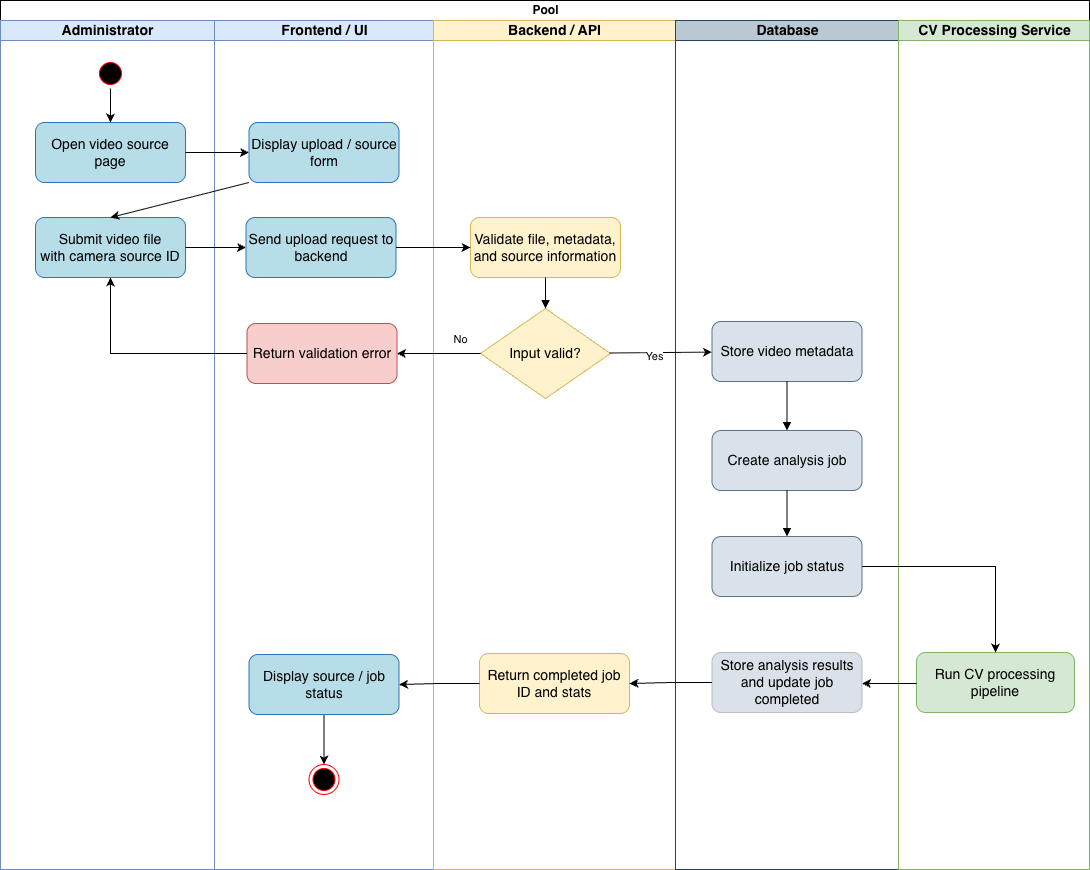
\includegraphics[width=\textwidth]{figures/activity-video-upload-analysis.png}
    \caption{Activity diagram for video upload and analysis job creation}
    \label{fig:activity-video-upload-analysis}
\end{figure}

\paragraph{Activity Diagram for Zone Configuration} Figure~\ref{fig:activity-zone-configuration} presents the swimlane UML activity diagram for the zone configuration process. The purpose of this diagram is to describe how an administrator defines monitored areas in the system before pedestrian movement analysis is performed. In the Smart Pedestrian Flow Monitoring and Analytics System, zones represent meaningful areas in a venue, such as entrances, corridors, booths, waiting areas, or exits. These zones are necessary because pedestrian trajectories alone are not sufficient for decision-making; the system must map raw movement coordinates to specific spatial regions in order to calculate zone-based counts, density, dwell time, and transition flows.

The diagram separates the responsibilities of the Administrator, System/Backend, and Database. The administrator selects a video frame or floor map, draws polygon boundaries, and enters zone metadata such as zone name, zone type, and density threshold. The system then validates whether the polygon and metadata are valid. If the zone definition is invalid, the system returns an error and asks the administrator to correct the input. If the zone is valid, the system stores the zone boundary, saves its metadata, and links the zone to the selected video, camera, or floor context.

The meaning of this figure is to show that zone configuration is a required preparation step before automated pedestrian flow analytics can be generated. By clearly defining zones, the system can later determine where each pedestrian is located, identify movements from one zone to another, detect overcrowded areas, and produce meaningful dashboard visualizations and reports.

\begin{figure}[H]
    \centering
    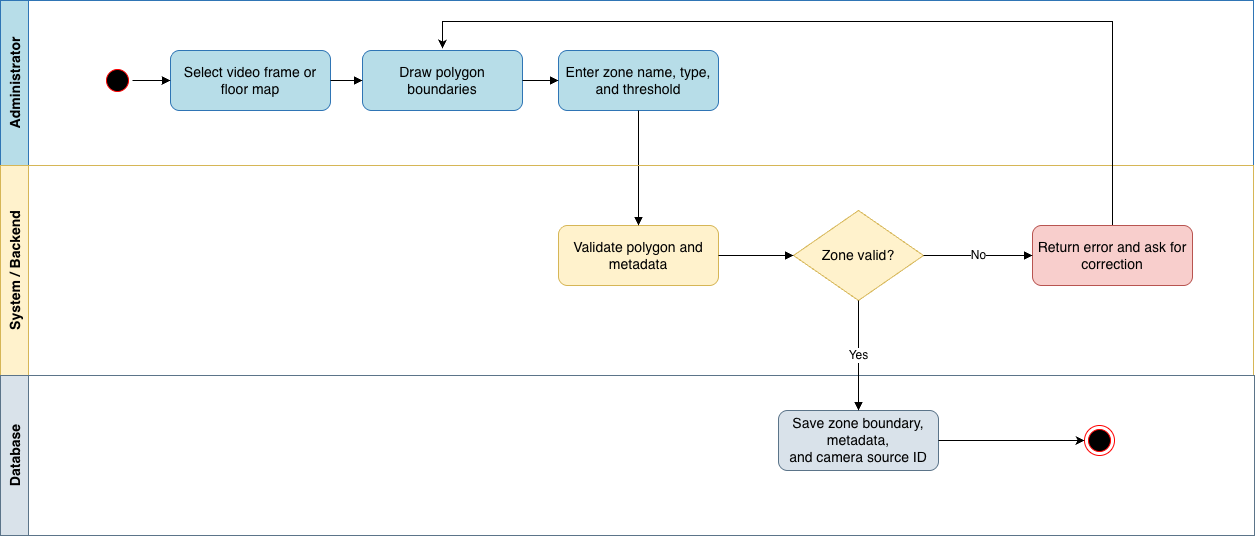
\includegraphics[width=\textwidth]{figures/activity-zone-configuration.png}
    \caption{Swimlane UML activity diagram for zone configuration}
    \label{fig:activity-zone-configuration}
\end{figure}

\paragraph{Activity Diagram for Pedestrian Analysis} 
Figure~\ref{fig:activity-pedestrian-analysis} presents the swimlane activity diagram for the pedestrian detection, tracking, and analysis workflow. The diagram separates the responsibilities of the backend job controller, database/storage, computer vision processing service, analytics engine, and frontend dashboard. The workflow starts when the backend retrieves a pending analysis job and requests the related video file and zone configuration from the database. If the required resources are not available, the system marks the job as failed and stores the error information.

When the required resources are available, the computer vision service reads video frames, detects pedestrians, assigns anonymous tracking IDs, and maps pedestrian positions to the configured zones. The generated trajectory points are saved for later inspection and analytics computation. The analytics engine then calculates zone counts, dwell time, density, transition flows, heatmap data, and alerts. After the job is completed, the backend updates the job status and the frontend dashboard displays the processed analytics results to the user.

\begin{figure}[H]
    \centering
    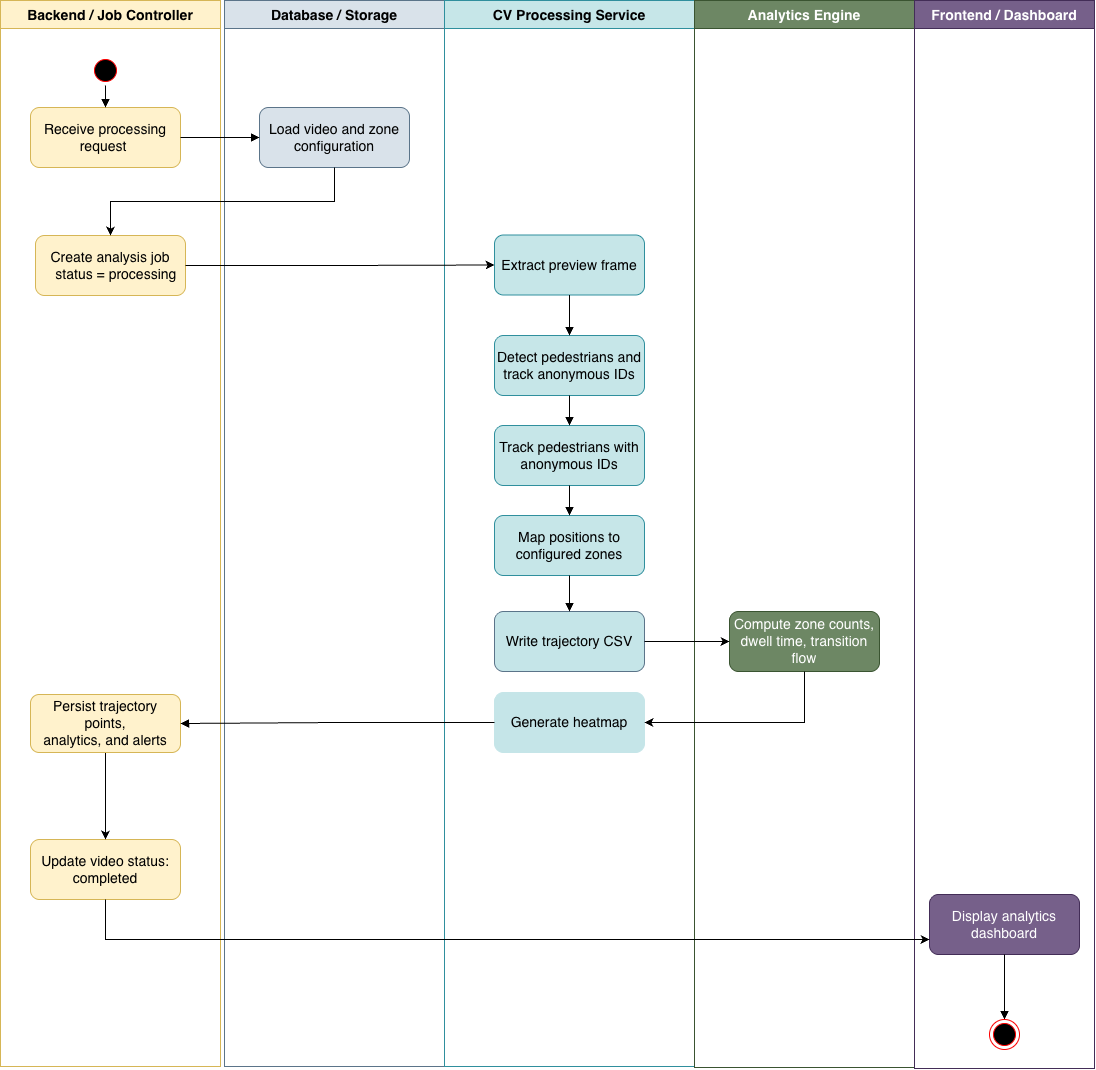
\includegraphics[width=\textwidth]{figures/activity-pedestrian-analysis.png}
    \caption{Swimlane UML activity diagram for pedestrian detection, tracking and analysis}
    \label{fig:activity-pedestrian-analysis}
\end{figure}

\subsection*{Business Function Diagram}
\begin{figure}[H]
    \centering
    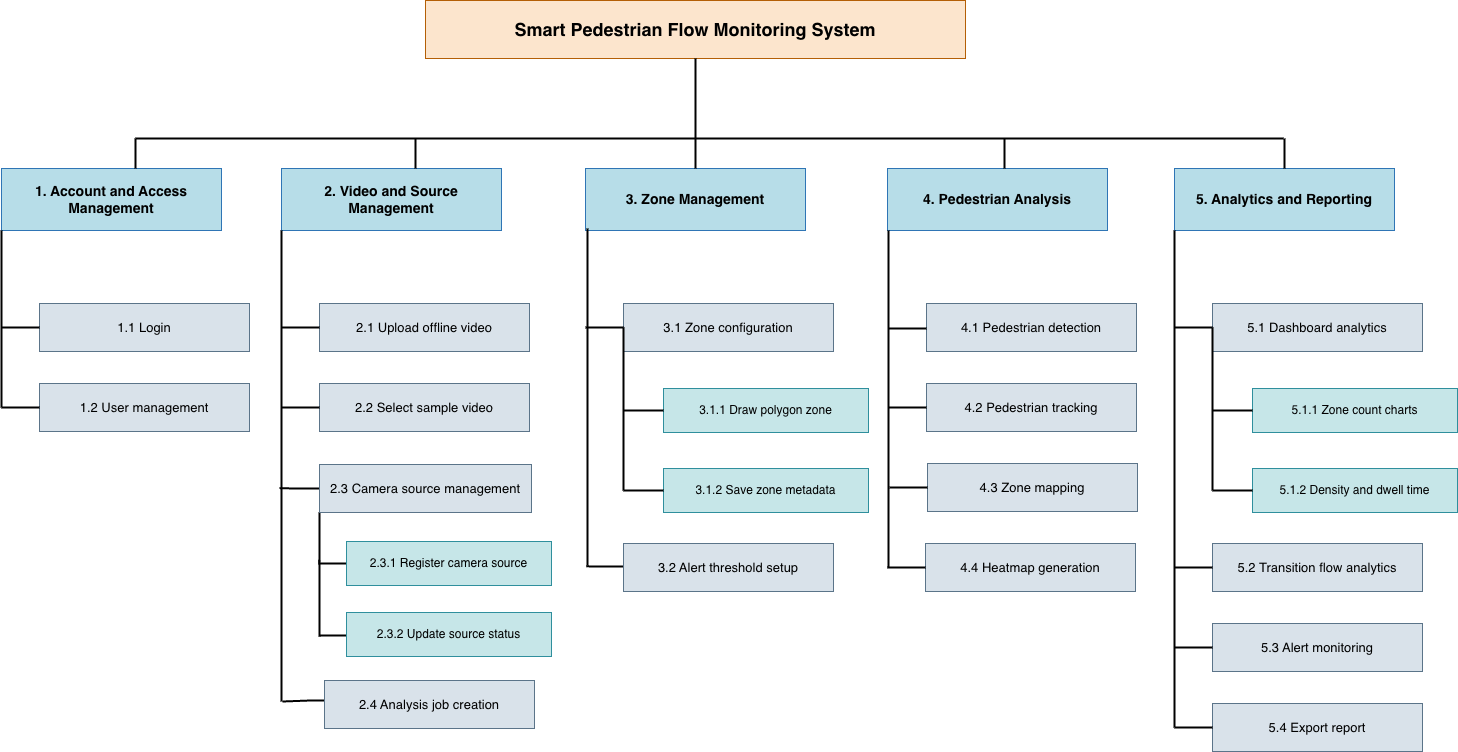
\includegraphics[width=\textwidth]{figures/business-function-diagram.png}
    \caption{Bussiness Function Diagram (BFD)}
    \label{fig:business-function}
\end{figure}

\subsection*{Business Function Decomposition Table}

\begin{small}
\setlength{\tabcolsep}{4pt}
\renewcommand{\arraystretch}{1.25}

\begin{longtable}{|>{\centering\arraybackslash}p{1.2cm}|
                  >{\raggedright\arraybackslash}p{4.0cm}|
                  >{\raggedright\arraybackslash}p{6.0cm}|
                  >{\raggedright\arraybackslash}p{3.0cm}|}
\hline
\rowcolor{HeaderBlue}
\textbf{No.} & \textbf{Business Function} & \textbf{Description} & \textbf{Implementation Status} \\
\hline
\endfirsthead

\hline
\rowcolor{HeaderBlue}
\textbf{No.} & \textbf{Business Function} & \textbf{Description} & \textbf{Implementation Status} \\
\hline
\endhead

\textbf{1} & 
\textbf{Administration and Access} & 
This function group manages access to the system and basic user information. It ensures that only registered users can use the demo application. & 
Implemented \\
\hline

1.1 & 
Login & 
Allow users to log in to the system using a username and password before accessing the video analysis functions. & 
Implemented \\
\hline

1.2 & 
User management & 
Store and manage user accounts in a database. The administrator can create, view, update, or delete user accounts at a basic level. & 
Implemented with database \\
\hline

\textbf{2} & 
\textbf{Video Source Management} & 
This function group manages the video input used for pedestrian flow analysis. In the demo, the system works with one offline video source. & 
Partially implemented \\
\hline

2.1 & 
Upload offline video & 
Allow users to upload a local video file for analysis. The uploaded video is used as the main input of the single-camera offline prototype. & 
Implemented \\
\hline

2.2 & 
Select sample video & 
Allow users to select a prepared sample video for quick demonstration without uploading their own file. & 
Implemented \\
\hline

2.3 & 
Camera source management & 
Manage real camera sources in a multi-camera monitoring environment, such as adding cameras and checking their availability. & 
Implemented \\
\hline

2.3.1 & 
Register camera source & 
Register information about a physical camera source, including camera name, location, and stream address. & 
Implemented \\
\hline

2.3.2 & 
Update source status & 
Update or display the current status of each camera source, such as active, inactive, or disconnected. & 
Future extension \\
\hline

2.4 & 
Analysis job creation & 
Create an analysis job after a video source is selected. The job includes the selected video, configured zones, and analysis settings. & 
Implemented \\
\hline

\textbf{3} & 
\textbf{Zone Management} & 
This function group allows users to define and manage monitoring zones used for zone-based pedestrian flow analytics. & 
Implemented \\
\hline

3.1 & 
Zone configuration & 
Allow users to define monitoring zones on the video frame, such as entrance, corridor, store area, or exit. & 
Implemented \\
\hline

3.1.1 & 
Draw/select polygon zone & 
Allow users to draw polygon zones or select predefined zones on the first frame of the uploaded video. & 
Implemented \\
\hline

3.1.2 & 
Save zone metadata & 
Save zone information such as zone name, polygon coordinates, and zone ID for later analysis. & 
Implemented \\
\hline

3.2 & 
Alert threshold setup & 
Allow users to configure simple alert thresholds, such as maximum people count per zone, density level, or dwell time threshold. & 
Implemented \\
\hline

\textbf{4} & 
\textbf{Pedestrian Analysis} & 
This function group processes video frames to detect pedestrians, track movement, map positions to zones, and generate visual movement patterns. & 
Implemented \\
\hline

4.1 & 
Pedestrian detection & 
Detect pedestrians in video frames using a computer vision model. The output includes bounding boxes and confidence scores. & 
Implemented \\
\hline

4.2 & 
Pedestrian tracking & 
Track detected pedestrians across frames using temporary anonymous track IDs. The system does not identify real personal identity. & 
Implemented \\
\hline

4.3 & 
Zone mapping & 
Map each tracked pedestrian to a monitoring zone based on the pedestrian position and the predefined zone coordinates. & 
Implemented \\
\hline

4.4 & 
Heatmap generation & 
Generate heatmap media showing areas where pedestrians frequently appear or move through. The current implementation stores both a heatmap image and a heatmap video for visualization rather than precise scientific measurement. & 
Implemented \\
\hline

\textbf{5} & 
\textbf{Flow Analytics and Reporting} & 
This function group summarizes pedestrian movement into charts, tables, alerts, and exported reports. & 
Implemented \\
\hline

5.1 & 
Dashboard analytics & 
Display analysis results through a dashboard, including zone statistics, charts, heatmap video, transition information, and alerts. & 
Implemented \\
\hline

5.1.1 & 
Zone count charts & 
Show the number of pedestrians detected in each monitoring zone using charts or summary tables. & 
Implemented \\
\hline

5.1.2 & 
Zone occupancy over time & 
Show how the number of pedestrians in each zone changes over the video timeline. & 
Implemented \\
\hline

5.1.3 & 
Density and dwell time & 
Estimate zone density and approximate dwell time. Dwell time is calculated based on how long a temporary track ID stays inside a zone. & 
Implemented \\
\hline

5.2 & 
Transition flow analytics & 
Compute and display movement transitions between zones, such as Entrance to Corridor or Corridor to Exit. & 
Implemented \\
\hline

5.3 & 
Alert monitoring & 
Compare analysis results with predefined thresholds and display warnings when a zone becomes overcrowded or when density or dwell time exceeds the configured limit. & 
Implemented as offline demo alert \\
\hline

5.4 & 
Export results/report & 
Export analysis results, such as zone counts, transition flows, alerts, and summary statistics, to CSV or report files. & 
Implemented \\
\hline

\end{longtable}
\end{small}

\section{Simple Project Plan}

\subsection*{Work Plan}

\begin{small}
\setlength{\tabcolsep}{4pt}
\renewcommand{\arraystretch}{1.25}

\begin{longtable}{|>{\centering\arraybackslash}p{1.0cm}|
                  >{\raggedright\arraybackslash}p{7.2cm}|
                  >{\centering\arraybackslash}p{2.4cm}|
                  >{\centering\arraybackslash}p{2.5cm}|}
\hline
\rowcolor{HeaderBlue}
\textbf{No.} & \textbf{Task} & \textbf{Estimated time (weeks)} & \textbf{People} \\
\hline
\endfirsthead

\hline
\rowcolor{HeaderBlue}
\textbf{No.} & \textbf{Task} & \textbf{Estimated time (weeks)} & \textbf{People} \\
\hline
\endhead

1 &
Project survey, scope definition, feasibility analysis, and team planning. &
1 &
6 \\
\hline

2 &
Requirement analysis, actor identification, use case modeling, and main workflow design. &
1 &
6 \\
\hline

3 &
System architecture, database schema, API design, frontend structure, and CV pipeline design. &
1 &
6 \\
\hline

4 &
Backend implementation: Express server, authentication, users, cameras, zones, upload, reprocess, analytics, alerts, jobs, and reports APIs. &
1 &
4 \\
\hline

5 &
Computer vision implementation: preview extraction, YOLOv8 tracking, trajectory export, analytics computation, zone mapping, and heatmap generation. &
2 &
3 \\
\hline

6 &
Frontend implementation: dashboard UI, source management, video upload, zone editor, charts, alerts, history, reports, users, and styling. &
3 &
3 \\
\hline

7 &
System integration, end-to-end testing, API smoke testing, manual regression testing, and bug fixing. &
2 &
6 \\
\hline

8 &
Final report, diagrams, screenshots, user guide, presentation slides, and demo rehearsal. &
2 &
6 \\
\hline

\end{longtable}
\end{small}

% =====================================================
% CHAPTER 2
% Revised to match the current FlowAI prototype
% =====================================================
\chapter{SOFTWARE REQUIREMENTS SPECIFICATION}

\section{General Introduction}

\subsection{System Actors}

\begin{longtable}{|c|p{3.6cm}|p{9.3cm}|}
\hline
\rowcolor{HeaderBlue}
\textbf{No.} & \textbf{Actor} & \textbf{Description} \\
\hline

1 & Administrator & Full-privilege user who manages accounts, camera sources, video uploads, zone configuration, analysis jobs, dashboards, alerts, and report exports. \\
\hline

2 & Analyst & Analysis-oriented user who views dashboards, heatmaps, transition flows, job details, report history, and exported reports. This actor cannot manage users, configure sources or zones, upload videos, or start analysis jobs. \\
\hline

3 & Security Staff & Operational monitoring user who views dashboards, camera results, multi-camera overview, and alerts. This actor can acknowledge alerts but cannot configure the system, run analysis jobs, or export reports. \\
\hline

\end{longtable}

\subsection{Supporting System Elements}

\begin{longtable}{|c|p{4.1cm}|p{8.8cm}|}
\hline
\rowcolor{HeaderBlue}
\textbf{No.} & \textbf{Element} & \textbf{Description} \\
\hline
1 & Video/Camera Source & A logical source of visual data. In the current prototype, a camera source stores metadata such as name, location, description, and status. Actual processing is performed on uploaded MP4 video files associated with a selected camera source. \\
\hline
2 & Computer Vision Processing Pipeline & Internal Python processing pipeline called by the backend. It extracts a preview frame, runs YOLOv8 pedestrian detection and ByteTrack tracking, computes analytics, persists anonymous trajectory data, and generates processed video and heatmap media. \\
\hline
3 & PostgreSQL Database & Internal persistent storage for users, camera sources, uploaded videos, zones, analysis jobs, anonymous tracks, trajectory points, zone counts, flow records, alerts, and report metadata. \\
\hline
\end{longtable}

\subsection{Main Use Cases}

\begin{table}[H]
\centering
\footnotesize
\setlength{\tabcolsep}{2.5pt}
\renewcommand{\arraystretch}{1.25}

\begin{tabularx}{\textwidth}{|
>{\centering\arraybackslash}p{0.6cm}|
>{\centering\arraybackslash}p{1.05cm}|
>{\raggedright\arraybackslash}p{2.35cm}|
>{\raggedright\arraybackslash}X|
>{\raggedright\arraybackslash}p{2.75cm}|}
\hline

\rowcolor{HeaderBlue}
\textbf{No.} & \textbf{Code} & \textbf{Use case} & \textbf{Description} & \textbf{Actor} \\
\hline

1 & UC-01 & Manage accounts 
& Create users, update user information, change user roles, and activate or deactivate accounts. 
& Administrator \\
\hline

2 & UC-02 & Login 
& Authenticate users and display functions according to their assigned role. 
& Administrator, Analyst, Security Staff \\
\hline

3 & UC-03 & Manage camera sources 
& Create, update, activate, deactivate, or delete logical camera sources used for video analysis. 
& Administrator \\
\hline

4 & UC-04 & Upload video and run analysis 
& Upload an MP4 video for a selected camera and start the pedestrian detection, tracking, analytics, and heatmap generation pipeline. 
& Administrator \\
\hline

5 & UC-05 & Configure zones and thresholds 
& Draw polygon or line zones on the video preview, assign zone names and types, and set density thresholds for each zone. 
& Administrator \\
\hline

6 & UC-06 & Reprocess analysis job 
& Re-run the analysis pipeline after zones or thresholds are updated for the selected camera. 
& Administrator \\
\hline

7 & UC-07 & View dashboard 
& View processed video, KPI cards, crowded zone, popular path, system status, heatmap video, and camera-specific analysis results. 
& Administrator, Analyst, Security Staff \\
\hline

8 & UC-08 & View multi-camera overview 
& Compare registered camera sources and open the latest completed analysis result of each camera. 
& Administrator, Analyst, Security Staff \\
\hline

9 & UC-09 & View analytics results 
& View zone counts, line-zone statistics, movement timeline, heatmap media, transition flow, and activity information. 
& Administrator, Analyst \\
\hline

10 & UC-10 & View job history and detail 
& Search, filter, and inspect historical analysis jobs, including job status, camera, video, zone counts, dwell time, density score, and transition records. 
& Administrator, Analyst \\
\hline

11 & UC-11 & Manage alerts 
& Review generated congestion alerts and acknowledge handled alerts during monitoring. 
& Administrator, Security Staff \\
\hline

12 & UC-12 & Export report 
& Export analysis results as CSV, open printable HTML report, download PDF report, and view generated report history. 
& Administrator, Analyst \\
\hline

\end{tabularx}

\caption{Main use cases of the Smart Pedestrian Flow Monitoring and Analytics prototype}
\label{tab:main-use-cases-flowai}
\end{table}


\section{Use Case Diagrams}

\subsection{Overall Use Case Diagram}

The overall use case diagram should show the main external actors: Administrator, Staff, and Data Analyst. The central system boundary
is the Smart Pedestrian Flow Monitoring and Analytics System. The core use cases include
login, account management, video/camera source management, zone configuration,
analysis job execution, dashboard viewing, multicamera overview, job history/detail,
heatmap viewing, transition-flow viewing, alert management, and report export.

\begin{figure}[H]
    \centering
    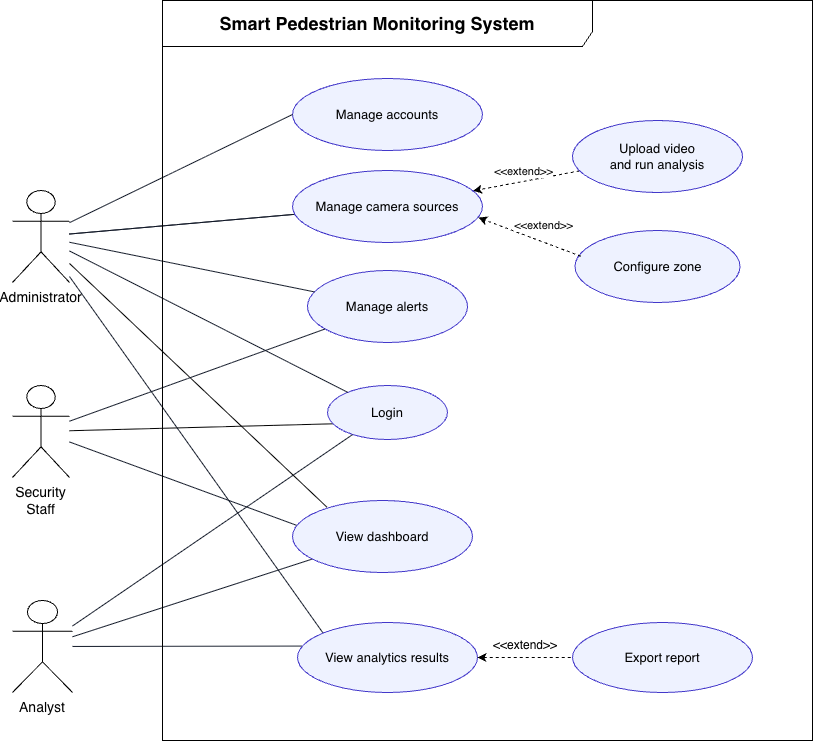
\includegraphics[width=0.85\textwidth]{figures/use-case-overall.png}
    \caption{Overall use case diagram}
    \label{fig:use-case-overall}
\end{figure}

\subsection{Level-2 Use Case Diagrams}

\begin{figure}[H]
    \centering
    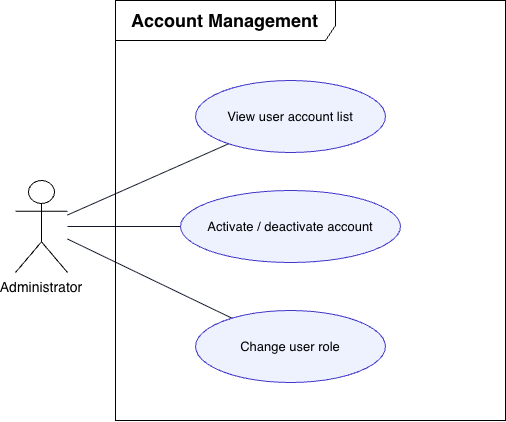
\includegraphics[width=0.6\textwidth]{figures/use-case-manage-accounts.png}
    \caption{Level-2 use case diagram: Manage accounts}
    \label{fig:use-case-manage-accounts}
\end{figure}

\begin{figure}[H]
    \centering
    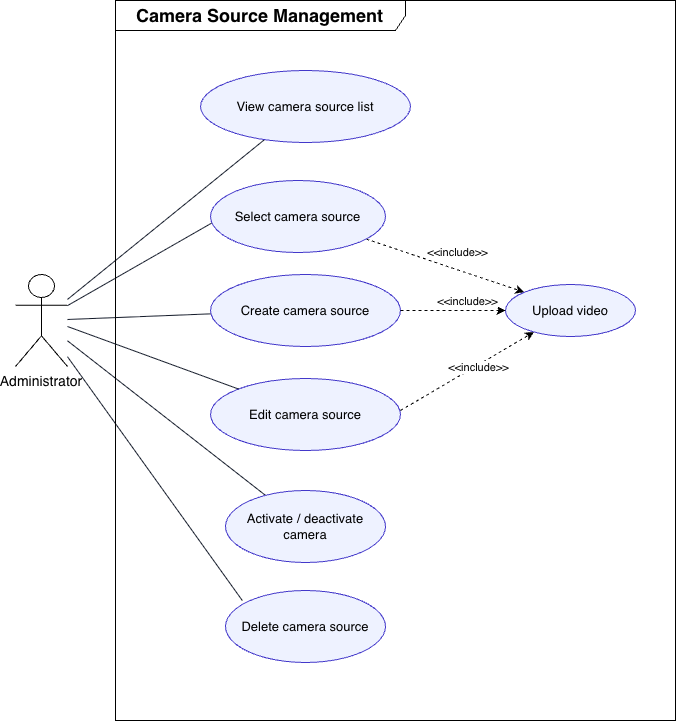
\includegraphics[width=0.75\textwidth]{figures/use-case-manage-sources.png}
    \caption{Level-2 use case diagram: Manage camera sources}
    \label{fig:use-case-manage-sources}
\end{figure}

\begin{figure}[H]
    \centering
    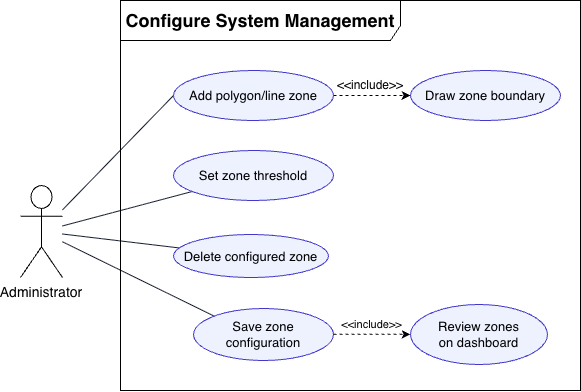
\includegraphics[width=0.65\textwidth]{figures/use-case-configure-system.png}
    \caption{Level-2 use case diagram: Configure system}
    \label{fig:use-case-configure-system}
\end{figure}

\begin{figure}[H]
    \centering
    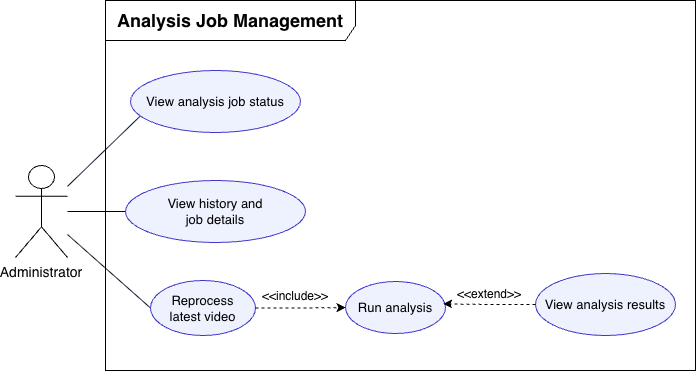
\includegraphics[width=0.8\textwidth]{figures/use-case-manage-analysis.png}
    \caption{Level-2 use case diagram: Manage analysis jobs}
    \label{fig:use-case-manage-analysis}
\end{figure}

\begin{figure}[H]
    \centering
    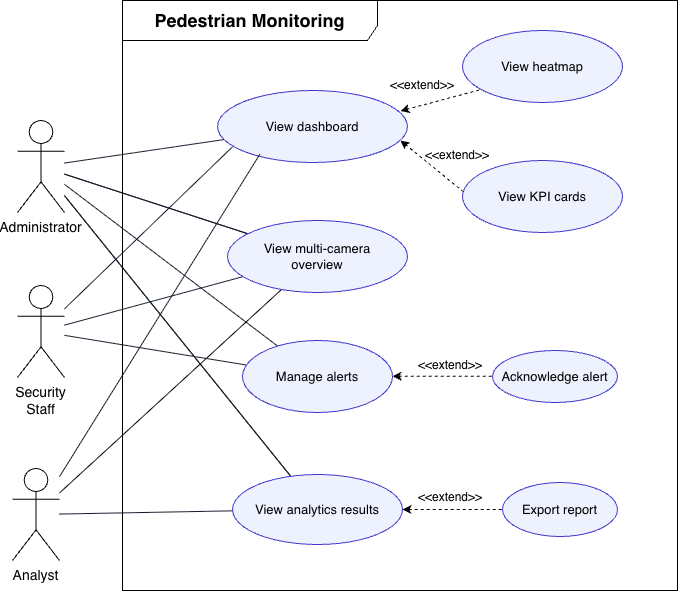
\includegraphics[width=0.65\textwidth]{figures/use-case-monitor-pedestrian-analytics.png}
    \caption{Level-2 use case diagram: Monitor pedestrian analytics}
    \label{fig:use-case-monitor-pedestrian-analytics}
\end{figure}

\section{Use Case Specifications}

\subsection{Use Case UC-01: Manage Accounts}
\begin{longtable}{|p{3.6cm}|p{10.4cm}|}
\hline
\rowcolor{HeaderBlue}\textbf{Item} & \textbf{Description} \\
\hline
Use case code & UC-01 \\
\hline
Use case name & Manage accounts \\
\hline
Actor & Administrator \\
\hline
Description & Allows the administrator to view user accounts, update user roles, and activate or deactivate users. The supported roles in the implemented system are \texttt{admin}, \texttt{analyst}, and \texttt{staff}. New self-registered accounts are created as Staff accounts by default. \\
\hline
Precondition & The administrator is logged in with an active account. \\
\hline
Main flow &
\begin{enumerate}
    \item Administrator opens the Users tab.
    \item The system displays the list of user accounts.
    \item Administrator reviews each user's name, email, role, and status.
    \item Administrator changes a user's role when necessary.
    \item Administrator activates or deactivates an account when necessary.
    \item The system saves the update and refreshes the user list.
\end{enumerate} \\
\hline
Alternative flow &
\begin{enumerate}
    \item If the current user is not an administrator, the system denies access to the Users tab or user-management API.
    \item If an update request contains an invalid role or status, the system rejects the request.
    \item If the selected user no longer exists, the system displays an error and reloads the account list.
\end{enumerate} \\
\hline
Postcondition & User account role or status is updated, and future access is controlled according to the updated role. \\
\hline
\end{longtable}

\subsection{Use Case UC-02: Login}
\begin{longtable}{|p{3.6cm}|p{10.4cm}|}
\hline
\rowcolor{HeaderBlue}\textbf{Item} & \textbf{Description} \\
\hline
Use case code & UC-02 \\
\hline
Use case name & Login \\
\hline
Actor & Administrator, Analyst, Security Staff \\
\hline
Description & Authenticates users and displays functions according to their assigned role. Administrators can access all functions. Analysts can view dashboards, analytics, multicamera overview, history, and reports. Security Staff can view dashboard, multicamera overview, and alerts. \\
\hline
Precondition & The user account exists and has active status. \\
\hline
Main flow &
\begin{enumerate}
    \item User opens the login page.
    \item User enters email and password.
    \item User submits the login form.
    \item The system validates the credentials and account status.
    \item If authentication succeeds, the system returns a session token and user profile.
    \item The frontend stores the token and opens the main interface.
    \item The system shows or hides menu items and actions according to the user's role.
\end{enumerate} \\
\hline
Alternative flow &
\begin{enumerate}
    \item If email or password is missing, the system asks the user to complete the required fields.
    \item If the credentials are incorrect, the system displays an authentication error.
    \item If the account is inactive, the system denies login.
    \item If the token expires or becomes invalid, the system returns the user to the login screen.
\end{enumerate} \\
\hline
Postcondition & The user is authenticated and can use only the functions permitted by their role. \\
\hline
\end{longtable}

\subsection{Use Case UC-03: Manage Camera Sources}
\begin{longtable}{|p{3.6cm}|p{10.4cm}|}
\hline
\rowcolor{HeaderBlue}\textbf{Item} & \textbf{Description} \\
\hline
Use case code & UC-03 \\
\hline
Use case name & Manage camera sources \\
\hline
Actor & Administrator \\
\hline
Description & Allows the administrator to create, select, activate, deactivate, or delete logical camera sources used for video analysis. Each camera source stores camera name, location, description, and status. \\
\hline
Precondition & The administrator is logged in. \\
\hline
Main flow &
\begin{enumerate}
    \item Administrator opens the Sources tab.
    \item The system displays the list of registered camera sources.
    \item Administrator enters camera name and location to create a new camera source.
    \item The system validates and saves the camera source.
    \item Administrator can select an existing camera source from the top camera selector.
    \item Administrator can activate, deactivate, or delete an existing camera source.
\end{enumerate} \\
\hline
Alternative flow &
\begin{enumerate}
    \item If the camera name is missing, the system rejects the creation request.
    \item If the selected camera is deleted, the system clears the current selection and refreshes related views.
    \item If a non-administrator attempts to manage camera sources, the system denies the action.
\end{enumerate} \\
\hline
Postcondition & Camera source information is updated and available for video upload, zone configuration, and monitoring. \\
\hline
\end{longtable}

\subsection{Use Case UC-04: Upload Video and Run Analysis}
\begin{longtable}{|p{3.6cm}|p{10.4cm}|}
\hline
\rowcolor{HeaderBlue}\textbf{Item} & \textbf{Description} \\
\hline
Use case code & UC-04 \\
\hline
Use case name & Upload video and run analysis \\
\hline
Actor & Administrator \\
\hline
Description & Allows the administrator to upload an MP4 video for a selected camera and start pedestrian detection, tracking, analytics generation, and heatmap generation. \\
\hline
Precondition & The administrator is logged in and a camera source is selected. \\
\hline
Main flow &
\begin{enumerate}
    \item Administrator selects a camera source.
    \item Administrator chooses an MP4 video file.
    \item Administrator clicks Upload Video.
    \item The system validates that a camera and video file are selected.
    \item The system uploads the video and starts the analysis job.
    \item The system displays processing status while the job is running.
    \item When processing finishes, the dashboard is updated with processed video, total people, heatmap video, and available analytics.
\end{enumerate} \\
\hline
Alternative flow &
\begin{enumerate}
    \item If no camera is selected, the system asks the administrator to select or create a camera source first.
    \item If no video file is selected, the system asks the administrator to choose a file.
    \item If the uploaded file is not a supported video, the system rejects the upload.
    \item If processing fails, the job is marked as failed and the error is shown in the job history.
\end{enumerate} \\
\hline
Postcondition & A new analysis job is created. If processing succeeds, processed media and analytics are available for the selected camera. \\
\hline
\end{longtable}

\subsection{Use Case UC-05: Configure Zones and Thresholds}
\begin{longtable}{|p{3.6cm}|p{10.4cm}|}
\hline
\rowcolor{HeaderBlue}\textbf{Item} & \textbf{Description} \\
\hline
Use case code & UC-05 \\
\hline
Use case name & Configure zones and thresholds \\
\hline
Actor & Administrator \\
\hline
Description & Allows the administrator to draw polygon zones or line zones on the video preview, assign zone names and types, delete incorrect zones, and set density thresholds for each zone. \\
\hline
Precondition & The administrator is logged in and a camera source is selected. A video preview should be available for accurate zone drawing. \\
\hline
Main flow &
\begin{enumerate}
    \item Administrator opens the System tab.
    \item The system displays the latest preview frame for the selected camera.
    \item Administrator chooses Polygon zone or Line zone drawing mode.
    \item Administrator clicks Add Zone and enters the zone name, type, and threshold.
    \item Administrator clicks Draw beside the zone to select it.
    \item Administrator clicks Draw Selected Zone and places points on the preview frame.
    \item Administrator adjusts the threshold from the threshold selector beside the zone when needed.
    \item Administrator deletes or clears a zone if the configuration is incorrect.
    \item Administrator clicks Save Zones.
    \item The system saves the zone configuration and updates dashboard overlays.
\end{enumerate} \\
\hline
Alternative flow &
\begin{enumerate}
    \item If no camera is selected, the system prevents saving zones.
    \item If no video has been uploaded for the camera, the preview area remains empty and zone drawing cannot be completed accurately.
    \item If the administrator uploads a new video for the same camera, previous zones are reset so the new video can be configured independently.
\end{enumerate} \\
\hline
Postcondition & Camera-specific polygon and line zones with thresholds are saved and available for reprocessing, dashboard visualization, analytics, and alerts. \\
\hline
\end{longtable}

\subsection{Use Case UC-06: Reprocess Analysis Job}
\begin{longtable}{|p{3.6cm}|p{10.4cm}|}
\hline
\rowcolor{HeaderBlue}\textbf{Item} & \textbf{Description} \\
\hline
Use case code & UC-06 \\
\hline
Use case name & Reprocess analysis job \\
\hline
Actor & Administrator \\
\hline
Description & Allows the administrator to re-run the analysis pipeline after zones or thresholds are updated for the selected camera. This ensures that dashboard cards, heatmap overlays, zone counts, transition flow, and alerts reflect the latest configuration. \\
\hline
Precondition & The selected camera has at least one uploaded video. \\
\hline
Main flow &
\begin{enumerate}
    \item Administrator modifies zone geometry or thresholds in the System tab.
    \item Administrator clicks Save Zones.
    \item The system saves the latest zone configuration.
    \item The system automatically starts reprocessing the latest uploaded video for the selected camera.
    \item The system updates the analysis job status while reprocessing.
    \item When reprocessing finishes, the system refreshes dashboard, analytics, alerts, history, and multicamera overview.
\end{enumerate} \\
\hline
Alternative flow &
\begin{enumerate}
    \item If the selected camera has no uploaded video, the system saves zones but informs the administrator to upload a video before analysis can be generated.
    \item If reprocessing fails, the failed job remains in history with its status and error information.
\end{enumerate} \\
\hline
Postcondition & A new analysis result is produced using the latest zone and threshold configuration, or the system records a failed reprocessing attempt. \\
\hline
\end{longtable}

\subsection{Use Case UC-07: View Dashboard}
\begin{longtable}{|p{3.6cm}|p{10.4cm}|}
\hline
\rowcolor{HeaderBlue}\textbf{Item} & \textbf{Description} \\
\hline
Use case code & UC-07 \\
\hline
Use case name & View dashboard \\
\hline
Actor & Administrator, Analyst, Security Staff \\
\hline
Description & Allows users to view processed video, KPI cards, crowded zone, popular path, system status, heatmap video, and camera-specific analysis results. \\
\hline
Precondition & The user is logged in. A completed analysis job is required to show processed media and analytics. \\
\hline
Main flow &
\begin{enumerate}
    \item User opens the Dashboard tab.
    \item User selects a camera source from the camera selector.
    \item The system loads the latest completed analysis result for the selected camera.
    \item The system displays total people, crowded zone, popular path, and congestion status.
    \item The system displays processed video and heatmap video when available.
    \item The system updates dashboard information according to the selected camera or opened historical job.
\end{enumerate} \\
\hline
Alternative flow &
\begin{enumerate}
    \item If no camera is selected, the dashboard remains in an empty or neutral state.
    \item If the selected camera has no completed job, processed video and analytics panels remain empty.
    \item If zones are not configured, zone-based dashboard values remain neutral or unavailable.
\end{enumerate} \\
\hline
Postcondition & User can monitor the latest pedestrian flow status for the selected camera or job. \\
\hline
\end{longtable}

\subsection{Use Case UC-08: View Multi-camera Overview}
\begin{longtable}{|p{3.6cm}|p{10.4cm}|}
\hline
\rowcolor{HeaderBlue}\textbf{Item} & \textbf{Description} \\
\hline
Use case code & UC-08 \\
\hline
Use case name & View multi-camera overview \\
\hline
Actor & Administrator, Analyst, Security Staff \\
\hline
Description & Allows users to compare registered camera sources and open the latest completed analysis result of each camera. \\
\hline
Precondition & User is logged in and at least one camera source exists. \\
\hline
Main flow &
\begin{enumerate}
    \item User opens the Multicam tab.
    \item The system displays registered camera sources.
    \item For each camera with a completed job, the system displays processed video, total people, peak zone, popular path, and alert count.
    \item User selects a camera card to open its latest completed job on the Dashboard.
\end{enumerate} \\
\hline
Alternative flow &
\begin{enumerate}
    \item If no camera source exists, the system displays an empty state.
    \item If a camera has no completed job, the system displays camera metadata without analytics.
\end{enumerate} \\
\hline
Postcondition & User can compare monitoring status and open detailed results for a selected camera. \\
\hline
\end{longtable}

\subsection{Use Case UC-09: View Analytics Results}
\begin{longtable}{|p{3.6cm}|p{10.4cm}|}
\hline
\rowcolor{HeaderBlue}\textbf{Item} & \textbf{Description} \\
\hline
Use case code & UC-09 \\
\hline
Use case name & View analytics results \\
\hline
Actor & Administrator, Analyst \\
\hline
Description & Allows users to view polygon-zone counts, line-zone statistics, movement timeline, heatmap media, transition flow, alerts, and activity information for completed analysis jobs. \\
\hline
Precondition & User is logged in as Administrator or Analyst. A completed job is available for the selected camera or historical job. \\
\hline
Main flow &
\begin{enumerate}
    \item User opens the Analytics tab.
    \item The system loads analytics for the selected camera or selected job.
    \item The system displays polygon zone analytics when polygon zones exist.
    \item The system displays line zone analytics when line zones exist.
    \item The system displays movement timeline, transition flow, alerts, and activity feed.
    \item User reviews the analytics to identify congestion, movement trends, and common paths.
\end{enumerate} \\
\hline
Alternative flow &
\begin{enumerate}
    \item If no completed job exists, analytics panels remain empty.
    \item If no polygon zones are configured, the polygon-zone panel displays no polygon-zone data.
    \item If no line zones are configured, the line-zone panel displays no line-zone data.
    \item If Security Staff attempts to access analytics, the system hides or denies the function according to role permissions.
\end{enumerate} \\
\hline
Postcondition & User can interpret pedestrian movement patterns and zone-level statistics for the selected camera or job. \\
\hline
\end{longtable}

\subsection{Use Case UC-10: View Job History and Detail}
\begin{longtable}{|p{3.6cm}|p{10.4cm}|}
\hline
\rowcolor{HeaderBlue}\textbf{Item} & \textbf{Description} \\
\hline
Use case code & UC-10 \\
\hline
Use case name & View job history and detail \\
\hline
Actor & Administrator, Analyst \\
\hline
Description & Allows users to search, filter, and inspect historical analysis jobs, including job status, camera, video, zone counts, dwell time, density score, and transition records. \\
\hline
Precondition & User is logged in as Administrator or Analyst, and analysis jobs exist. \\
\hline
Main flow &
\begin{enumerate}
    \item User opens the History tab.
    \item User enters a search keyword or selects a status filter.
    \item The system displays matching analysis jobs.
    \item User selects a job to view details.
    \item The system displays job metadata, status, zone analytics, transition records, alerts, and track summary.
    \item User can open the selected job on the Dashboard for detailed visual inspection.
\end{enumerate} \\
\hline
Alternative flow &
\begin{enumerate}
    \item If no job matches the filter, the system displays an empty state.
    \item If a job failed, the system displays its failed status and available error information.
    \item If Security Staff attempts to access history, the system hides or denies the function according to role permissions.
\end{enumerate} \\
\hline
Postcondition & User can audit previous analysis jobs and reload a selected job result. \\
\hline
\end{longtable}

\subsection{Use Case UC-11: Manage Alerts}
\begin{longtable}{|p{3.6cm}|p{10.4cm}|}
\hline
\rowcolor{HeaderBlue}\textbf{Item} & \textbf{Description} \\
\hline
Use case code & UC-11 \\
\hline
Use case name & Manage alerts \\
\hline
Actor & Administrator, Security Staff \\
\hline
Description & Allows users to review generated congestion alerts and acknowledge handled alerts during monitoring. Alerts are created when zone counts exceed configured thresholds. \\
\hline
Precondition & User is logged in as Administrator or Security Staff. At least one analysis job has been completed. \\
\hline
Main flow &
\begin{enumerate}
    \item User opens the Alerts tab.
    \item The system displays open congestion alerts with zone name, severity, threshold, actual count, and time.
    \item User reviews the alert information.
    \item User clicks Acknowledge after the alert has been handled.
    \item The system updates the alert status and changes the acknowledgement control to the handled state.
\end{enumerate} \\
\hline
Alternative flow &
\begin{enumerate}
    \item If no alert exists, the system displays an empty alert state.
    \item If acknowledgement fails, the alert remains open.
    \item If Analyst attempts to acknowledge an alert, the system denies the action according to role permissions.
\end{enumerate} \\
\hline
Postcondition & The selected alert is marked as acknowledged and no longer requires immediate handling. \\
\hline
\end{longtable}

\subsection{Use Case UC-12: Export Report}
\begin{longtable}{|p{3.6cm}|p{10.4cm}|}
\hline
\rowcolor{HeaderBlue}\textbf{Item} & \textbf{Description} \\
\hline
Use case code & UC-12 \\
\hline
Use case name & Export report \\
\hline
Actor & Administrator, Analyst \\
\hline
Description & Allows users to export completed analysis results as CSV or PDF reports and view generated report history. \\
\hline
Precondition & User is logged in as Administrator or Analyst, and at least one completed analysis job exists. \\
\hline
Main flow &
\begin{enumerate}
    \item User opens the Reports tab.
    \item User selects or keeps the current camera/job context.
    \item User clicks Export CSV Report or Download PDF Report.
    \item The system generates a report using the selected job's summary, zone counts, transition flow, dwell time, density score, timeline, and congestion status.
    \item The system downloads the requested report file.
    \item The Reports tab displays the generated report history.
\end{enumerate} \\
\hline
Alternative flow &
\begin{enumerate}
    \item If no completed job exists, the system displays an empty state or returns an error indicating that no report data is available.
    \item If the user's authentication token is missing or invalid, the export request is rejected.
    \item If Security Staff attempts to export a report, the system hides or denies the function according to role permissions.
\end{enumerate} \\
\hline
Postcondition & The requested report is generated and report metadata is recorded for history tracking. \\
\hline
\end{longtable}

\subsection{Use Case UC-11: Manage Alert Thresholds and Alerts}
\begin{longtable}{|p{3.6cm}|p{10.4cm}|}
\hline
\rowcolor{HeaderBlue}\textbf{Item} & \textbf{Description} \\
\hline
Use case code & UC-11 \\
\hline
Use case name & Manage alert thresholds and alerts \\
\hline
Actor & Administrator, Operator \\
\hline
Description & Allows authorized users to configure zone thresholds, review generated congestion alerts, and acknowledge handled alerts. Analysts may view alert information as part of dashboards and reports but cannot configure thresholds. \\
\hline
Precondition & A camera source and zones exist. \\
\hline
Main flow &
\begin{enumerate}
    \item User opens System and sets a threshold for each zone.
    \item User saves the zone configuration.
    \item During analysis, the backend compares zone counts with thresholds.
    \item If a count exceeds the threshold, the system creates an alert with severity \texttt{warning} or \texttt{danger}.
    \item User opens the Alerts tab and reviews alert details.
    \item User acknowledges an alert after handling it.
\end{enumerate} \\
\hline
Alternative flow & If no alert exists, the Alerts tab displays an empty state. If acknowledgement fails, the system keeps the alert open. \\
\hline
Postcondition & Thresholds are stored per zone and alert status is updated in PostgreSQL. \\
\hline
\end{longtable}

\subsection{Use Case UC-12: Export Report}
\begin{longtable}{|p{3.6cm}|p{10.4cm}|}
\hline
\rowcolor{HeaderBlue}\textbf{Item} & \textbf{Description} \\
\hline
Use case code & UC-12 \\
\hline
Use case name & Export report \\
\hline
Actor & Administrator, Operator, Analyst \\
\hline
Description & Exports analytics for a completed job in CSV, printable HTML, or backend-generated PDF format. The system also stores report metadata for report history. \\
\hline
Precondition & User is authenticated and at least one completed analysis job exists. \\
\hline
Main flow &
\begin{enumerate}
    \item User opens the Reports tab.
    \item User selects a camera and/or job.
    \item User chooses CSV export, printable report, or PDF download.
    \item The backend retrieves job statistics, zone counts, transitions, dwell times, density scores, timeline, and congestion status.
    \item The backend creates report metadata in the \texttt{reports} table.
    \item The system returns the generated file or opens the printable report page.
    \item The Reports tab displays generated report history.
\end{enumerate} \\
\hline
Alternative flow & If no completed job exists, the system returns an error or empty state indicating that no analysis result is available. \\
\hline
Postcondition & Report output is generated and report metadata is stored. \\
\hline
\end{longtable}

\section{Non-Functional Requirements}

\subsection*{Functionality}
\begin{itemize}
    \item The system shall support multiple user roles, including Administrator, Security Staff/ Operator, and Data Analyst/Facility Planner.
    \item Management functions shall only be available to authenticated users with appropriate permissions.
    \item The system shall validate user input before saving it to the database.
    \item All functions that interact with the database shall have error-handling mechanisms.
    \item The system shall support logical camera source management and uploaded MP4 video processing.
    \item The system shall store pedestrian records using anonymous track IDs instead of personal identities.
\end{itemize}

\subsection*{Usability}
\begin{itemize}
    \item The interface shall be understandable for non-technical administrators, analysts, and staff users.
    \item The dashboard shall present analytics using clear KPI cards, charts, heatmaps, tables, status messages, and job history views.
    \item Error messages shall clearly indicate the field or operation causing the error.
    \item The interface language confirmed for the final prototype is English.
\end{itemize}

\subsection*{Performance}
\begin{itemize}
    \item The system shall process short uploaded demo videos within an acceptable time limit for classroom demonstration.
    \item The current prototype performs offline batch processing rather than real-time stream processing.
    \item The dashboard shall load stored analytics results from PostgreSQL in a reasonable response time for local demonstration.
    \item Recommended demo videos should be short, preferably 10--60 seconds, to keep YOLOv8 processing practical on local hardware.
\end{itemize}

\subsection*{Reliability}
\begin{itemize}
    \item The system shall handle invalid video files, missing zone configuration, failed analysis jobs, and empty detection results.
    \item The system shall preserve analysis job status so users can identify whether a job is uploaded, processing, completed, or failed.
    \item The system shall store generated media by job ID so historical dashboard results can be reloaded without being overwritten by later jobs.
    \item The system shall avoid data loss by using persistent storage for confirmed records.
\end{itemize}

\subsection*{Maintainability}
\begin{itemize}
    \item The system shall separate the user interface, backend/API logic, computer vision processing, analytics logic, and database access.
    \item The detection/tracking implementation shall be replaceable because the exact model/algorithm may change.
    \item Source code shall be organized into clear modules with readable naming and documentation.
\end{itemize}

\subsection*{Security and Privacy}
\begin{itemize}
    \item The system shall require user authentication for management functions.
    \item Role-based permission shall restrict sensitive operations such as user management, camera source management, video upload, zone configuration, and analysis job execution.
    \item The system shall not implement face recognition, biometric enrollment, identity matching, or personal identification.
    \item The system shall store only anonymous movement analytics, anonymous track IDs, zone names, trajectory points, and aggregate results for pedestrians.
    \item If real venue footage is used, close-up identifiable faces should be avoided or anonymized where possible, and production privacy/compliance review should be treated as future work.
\end{itemize}

\subsection*{Technical Constraints}
\begin{itemize}
    \item The system shall run as a local web application for the course demo environment.
    \item Confirmed frontend technology: HTML, CSS, and JavaScript served by the backend.
    \item Confirmed backend technology: Node.js with Express.
    \item Confirmed database: PostgreSQL.
    \item Confirmed CV detector: YOLOv8.
    \item Confirmed tracking algorithm: ByteTrack.
    \item Confirmed processing mode: offline uploaded MP4 video processing.
\end{itemize}

% =====================================================
% CHAPTER 3
% =====================================================
\chapter{REQUIREMENT ANALYSIS}
\label{chap:requirement-analysis}

This chapter analyzes the requirements of the Smart Pedestrian Flow Monitoring and Analytics System and transforms them into analysis-level models.
The purpose of this chapter is to identify the main analysis classes, user-system interactions, data entities, and processing scenarios required by the implemented project scope.
The current prototype focuses on an offline video analytics workflow with logical camera sources, role-based access control, configurable polygon and line zones, YOLO-based pedestrian detection, ByteTrack-based anonymous tracking, PostgreSQL persistence, dashboard analytics, alert monitoring, and report export.

The system is implemented as a web-based application with an Express.js backend, a browser-based frontend, PostgreSQL for persistent storage, and Python computer vision services for video processing.
Although the system supports multiple logical camera sources for comparing different locations or uploaded videos, the analysis input is an uploaded video file rather than a live camera stream.
Camera sources are therefore managed as metadata records, while video files are uploaded and processed as analysis jobs.

\section{Identifying Analysis Classes}
\label{sec:identifying-analysis-classes}

The analysis model separates the system into three types of classes: boundary classes, control classes, and entity classes.
Boundary classes represent user interface screens or external interaction points.
Control classes coordinate business logic and connect the interface with authentication, database operations, video processing, analytics computation, alerts, and reporting.
Entity classes represent persistent business data stored in PostgreSQL and generated media or output artifacts stored in the backend public directory.

\subsection*{Main Boundary Classes}

\begin{longtable}{|p{4.2cm}|p{9.6cm}|}
\hline
\rowcolor{HeaderBlue}
\textbf{Boundary Class} & \textbf{Responsibility} \\
\hline
LoginPage & Provides the login interface for authenticated access to the system. \\
\hline
UserManagementPage & Allows the administrator to create, view, update, and deactivate user accounts stored in PostgreSQL. \\
\hline
CameraSourcePage & Allows administrators to create, update, delete, and view logical camera sources. \\
\hline
VideoInputPage & Allows users to upload an offline video or select a prepared sample video for analysis. \\
\hline
ZoneConfigurationPage & Allows administrators to draw polygon or line zones on a preview frame, assign zone types, and configure zone-level thresholds. \\
\hline
AnalysisJobPage & Allows users to view analysis job history, job status, generated media, and detailed analytics for each processed
video. \\
\hline
DashboardPage & Displays the main analysis results, including KPI cards, processed video, realtime video-window statistics, zone count charts, transition flow, heatmap video, and congestion status. \\
\hline
MultiCameraOverview-Page & Displays the latest completed analysis result for each logical camera source and allows users to compare cameras. \\
\hline
HeatmapPage & Displays the generated heatmap video for a completed analysis job, with a heatmap image available as a static fallback. \\
\hline
FlowAnalyticsPage & Displays zone counts, transition flow, density score, dwell time, and timeline analytics. \\
\hline
AlertMonitoringPage & Displays generated alerts when a configured zone threshold is exceeded and allows alert acknowledgement. \\
\hline
ReportExportPage & Allows administrators and analysts to export completed analysis results as CSV, or backend-generated PDF reports. \\
\hline
\end{longtable}

\subsection*{Main Control Classes}

\begin{longtable}{|p{4.2cm}|p{9.6cm}|}
\hline
\rowcolor{HeaderBlue}
\textbf{Control Class} & \textbf{Responsibility} \\
\hline
AuthController & Handles login, password verification, session token creation, session validation, and role-based authorization. \\
\hline
UserController & Manages user account creation, role assignment, account status updates, and administrator-only user operations. \\
\hline
CameraSourceController & Manages logical camera source metadata such as name, location, description, and status. \\
\hline
VideoUploadController & Handles video file upload, video metadata persistence, and analysis job creation for the selected camera source. \\
\hline
ZoneController & Handles polygon and line zone persistence, normalized coordinates, zone metadata, and threshold settings. \\
\hline
AnalysisJobController & Creates and manages video analysis jobs, processing status, generated media paths, and job history. \\
\hline
PedestrianProcessingController & Coordinates preview extraction, YOLO-based pedestrian detection, ByteTrack-based tracking, analytics computation, trajectory persistence, and heatmap generation. \\
\hline
AnalyticsController & Retrieves stored analytics such as total people, zone counts, transition flows, timeline, dwell time, density score, and realtime video-window statistics. \\
\hline
AlertController & Compares zone counts with configured thresholds, creates alert records, retrieves alerts, and acknowledges alerts. \\
\hline
ReportController & Generates CSV, printable HTML, and PDF reports from completed analysis jobs and stores report export metadata. \\
\hline
DemoDataController & Seeds a complete synthetic demo dataset including camera source, zones, video metadata, analysis job, tracks, trajectory points, flow records, alerts, and media outputs. \\
\hline
\end{longtable}

\subsection*{Main Entity Classes}

\begin{longtable}{|p{4.2cm}|p{9.6cm}|}
\hline
\rowcolor{HeaderBlue}
\textbf{Entity Class} & \textbf{Responsibility} \\
\hline
User & Stores user account information such as full name, email, password hash, role, account status, and creation time. \\
\hline
Role & Represents user permission levels: administrator, analyst, and staff. \\
\hline
CameraSource & Represents a logical camera source with name, location, description, and status. \\
\hline
Video & Stores uploaded video metadata, including file name, original name, file path, camera source, upload status, and processing time. \\
\hline
Zone & Stores monitoring zone information, including camera source, zone name, zone type, polygon or line coordinates, grid position for ordering, and threshold value. \\
\hline
AnalysisJob & Stores analysis job metadata, selected video, camera source, processing status, start time, finish time, error message, aggregate analytics, and generated media paths. \\
\hline
PedestrianTrack & Stores anonymous temporary track IDs and frame range information for detected pedestrians. \\
\hline
TrajectoryPoint & Stores frame-level position points of a pedestrian track, including frame index, center coordinates, and mapped zone. \\
\hline
ZoneCount & Stores the total people count for each zone in an analysis job. \\
\hline
FlowRecord & Stores transition counts between zones, such as Lobby to Exit. \\
\hline
Alert & Stores generated alert records when zone counts exceed configured thresholds and stores acknowledgement information. \\
\hline
Report & Stores exported report metadata, including analysis job, camera source, generated user, report format, filters, and creation time. \\
\hline
\end{longtable}

\begin{figure}[H]
    \centering
    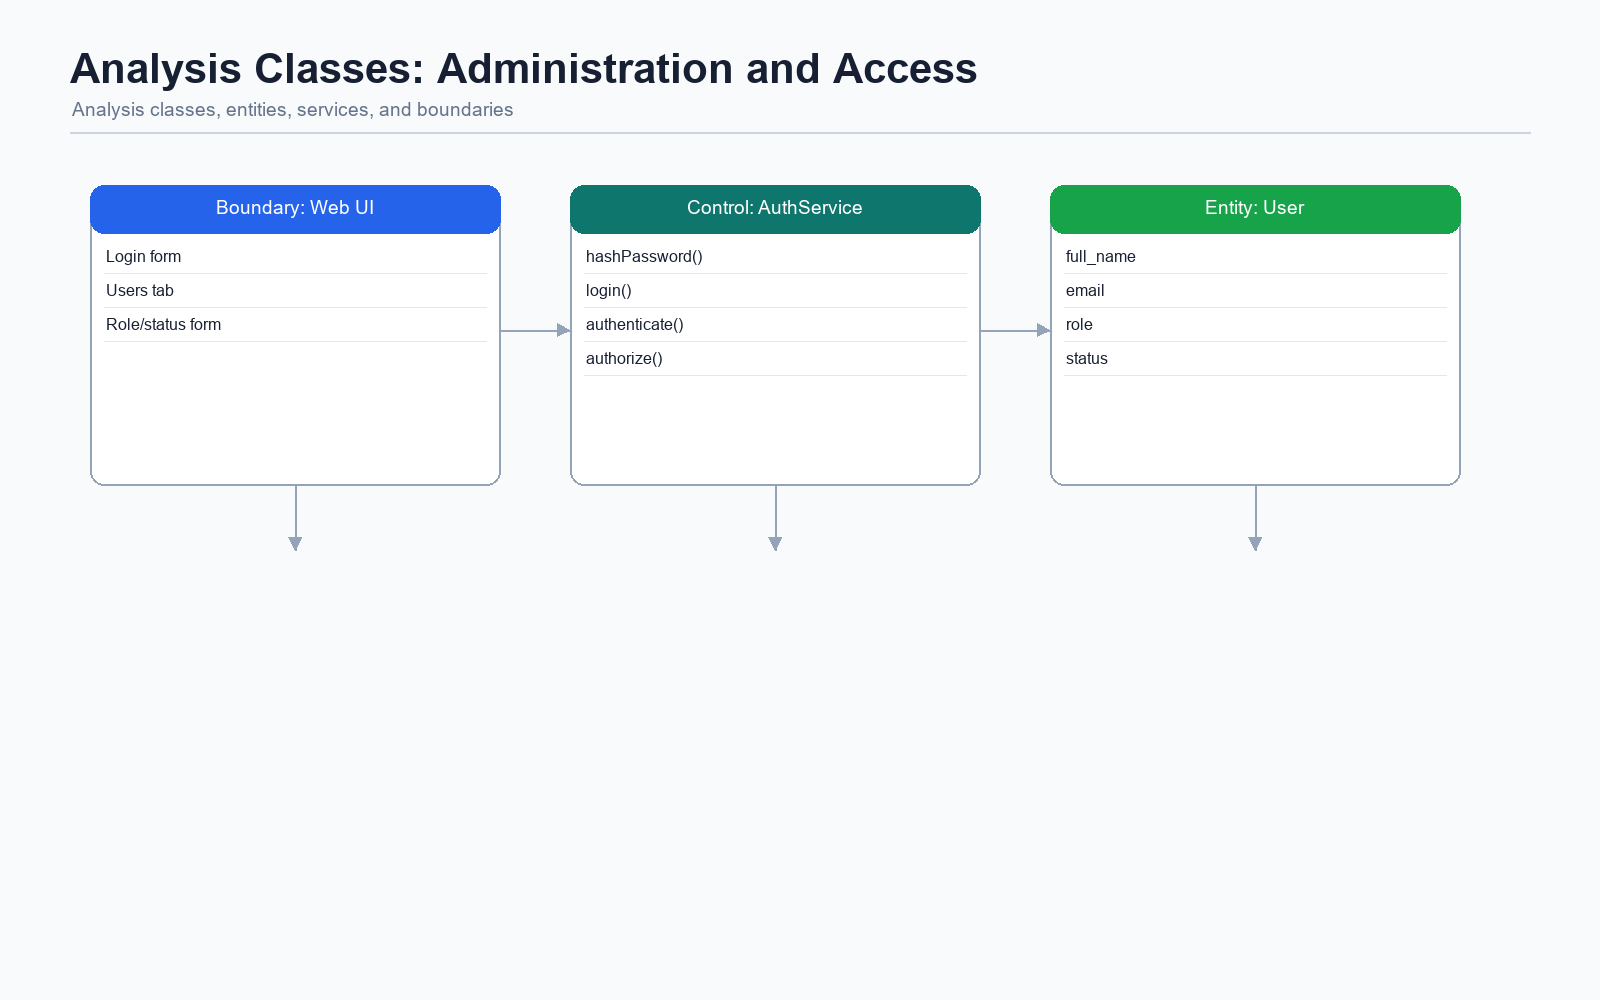
\includegraphics[width=\textwidth]{figures/analysis-class-administration.png}
    \caption{Analysis class decomposition for administration and access}
    \label{fig}
\end{figure}

\begin{figure}[H]
    \centering
    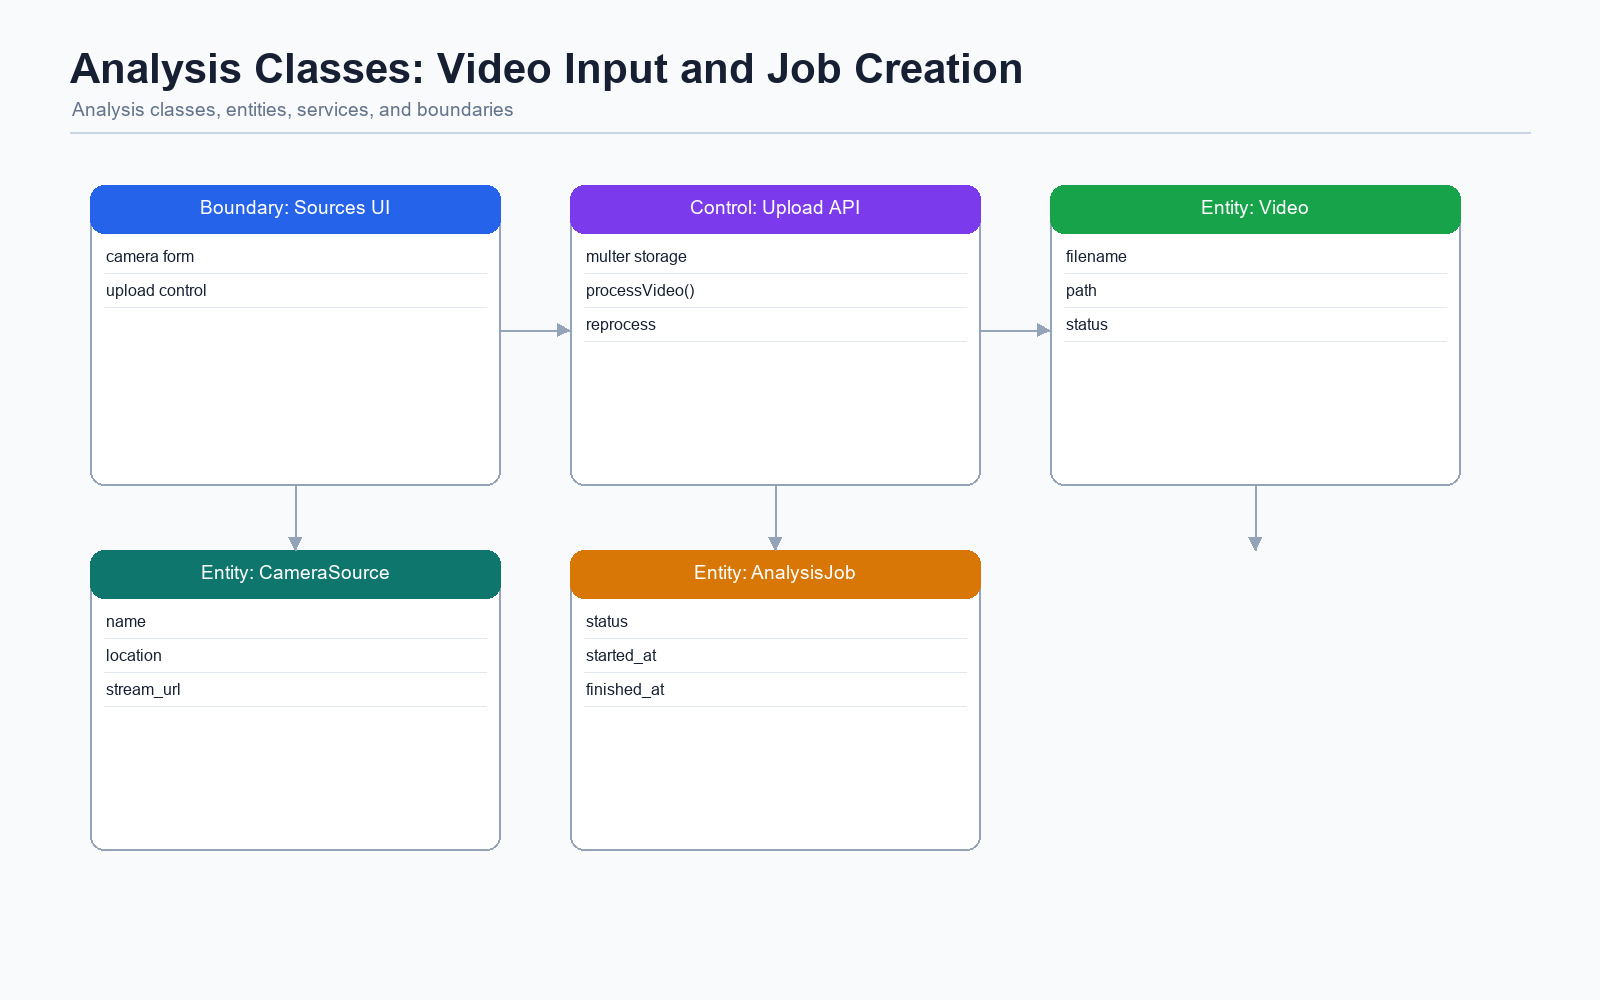
\includegraphics[width=\textwidth]{figures/analysis-class-video-input.png}
    \caption{Analysis class decomposition for video input and analysis job creation}
    \label{fig}
\end{figure}

\begin{figure}[H]
    \centering
    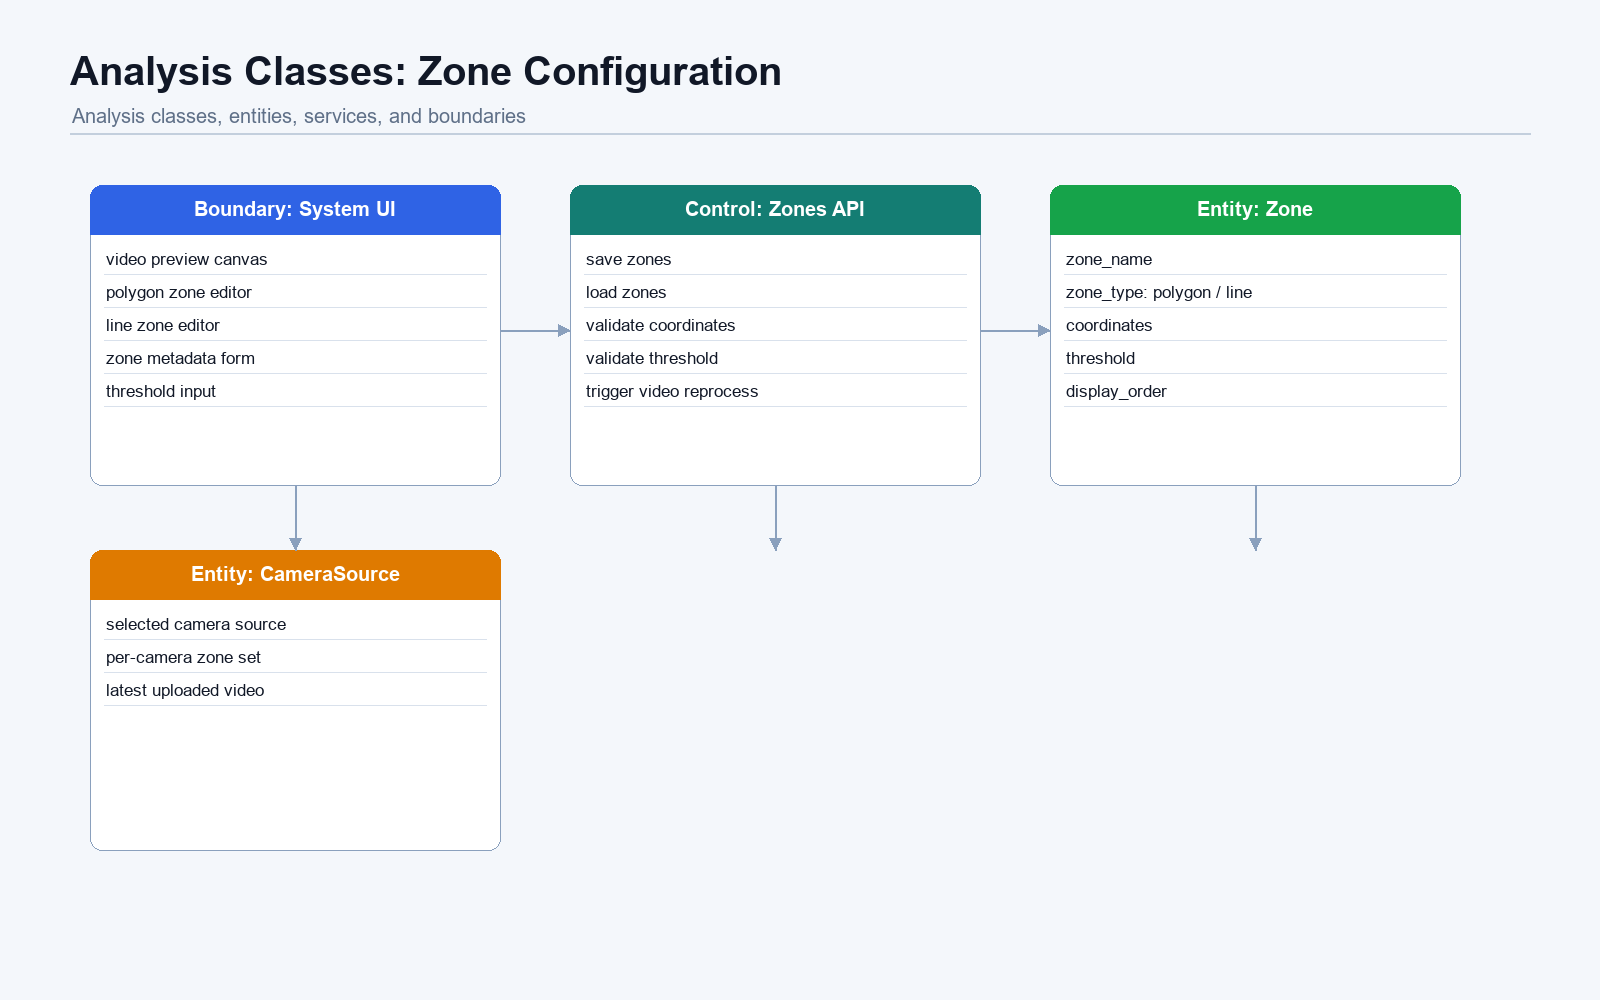
\includegraphics[width=\textwidth]{figures/analysis-class-zone-configuration.png}
    \caption{Analysis class decomposition for zone configuration and threshold setup}
    \label{fig}
\end{figure}

\begin{figure}[H]
    \centering
    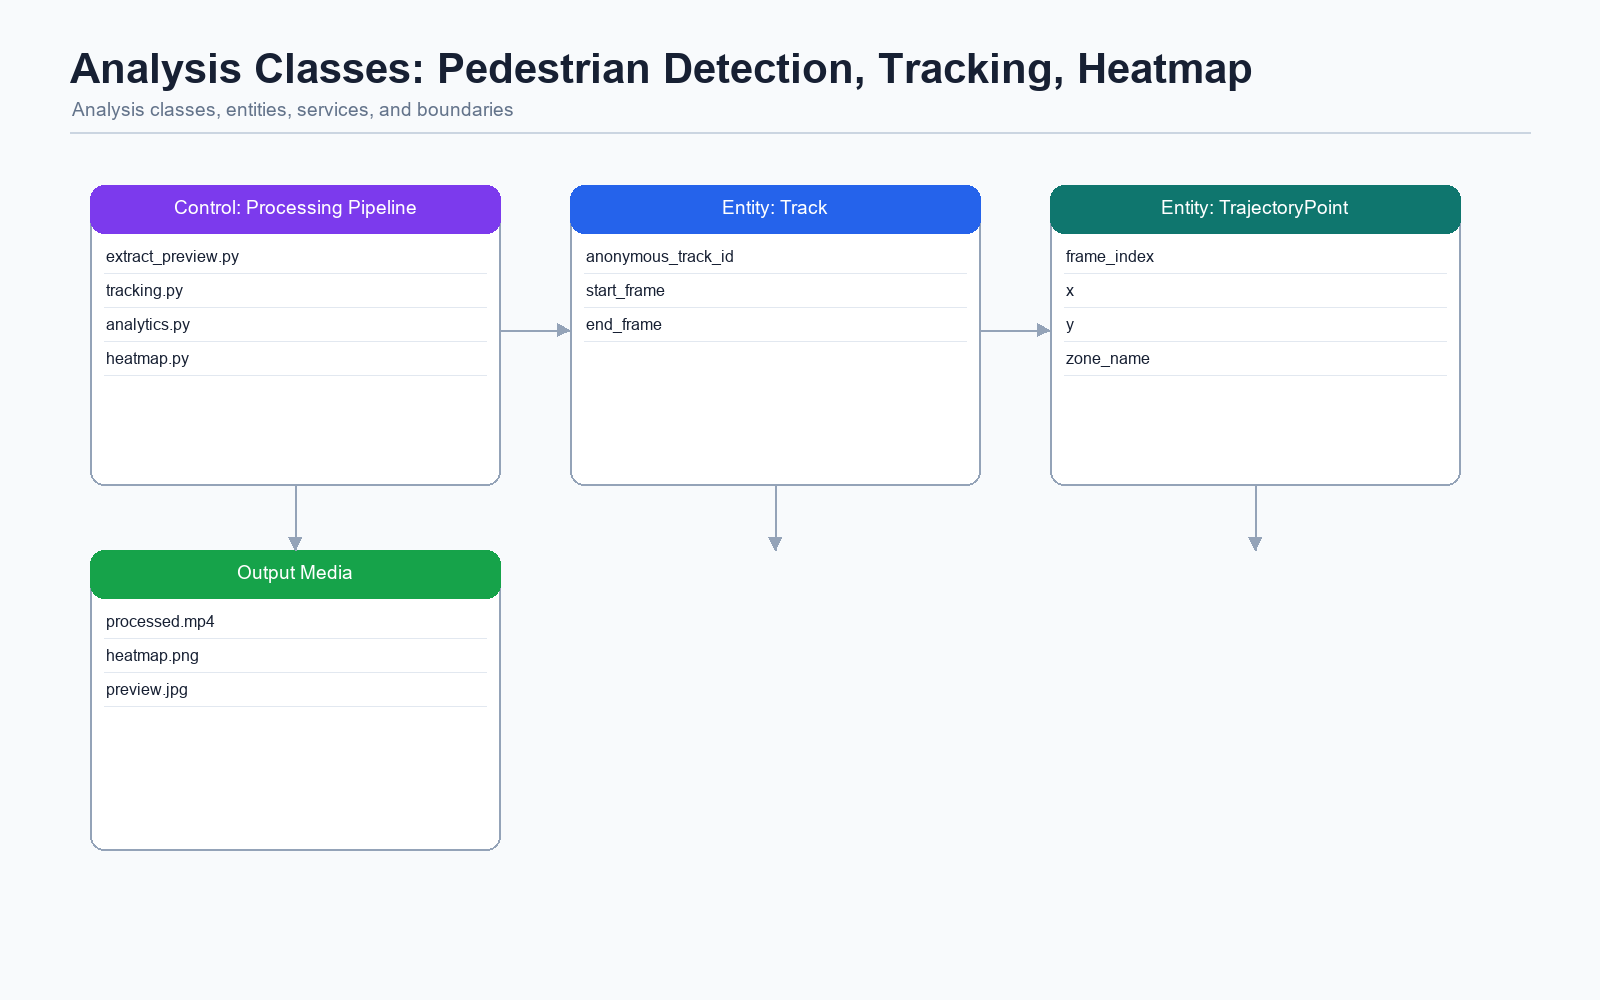
\includegraphics[width=\textwidth]{figures/analysis-class-pedestrian-analysis.png}
    \caption{Analysis class decomposition for pedestrian detection, tracking, and heatmap generation}
    \label{fig}
\end{figure}

\begin{figure}[H]
    \centering
    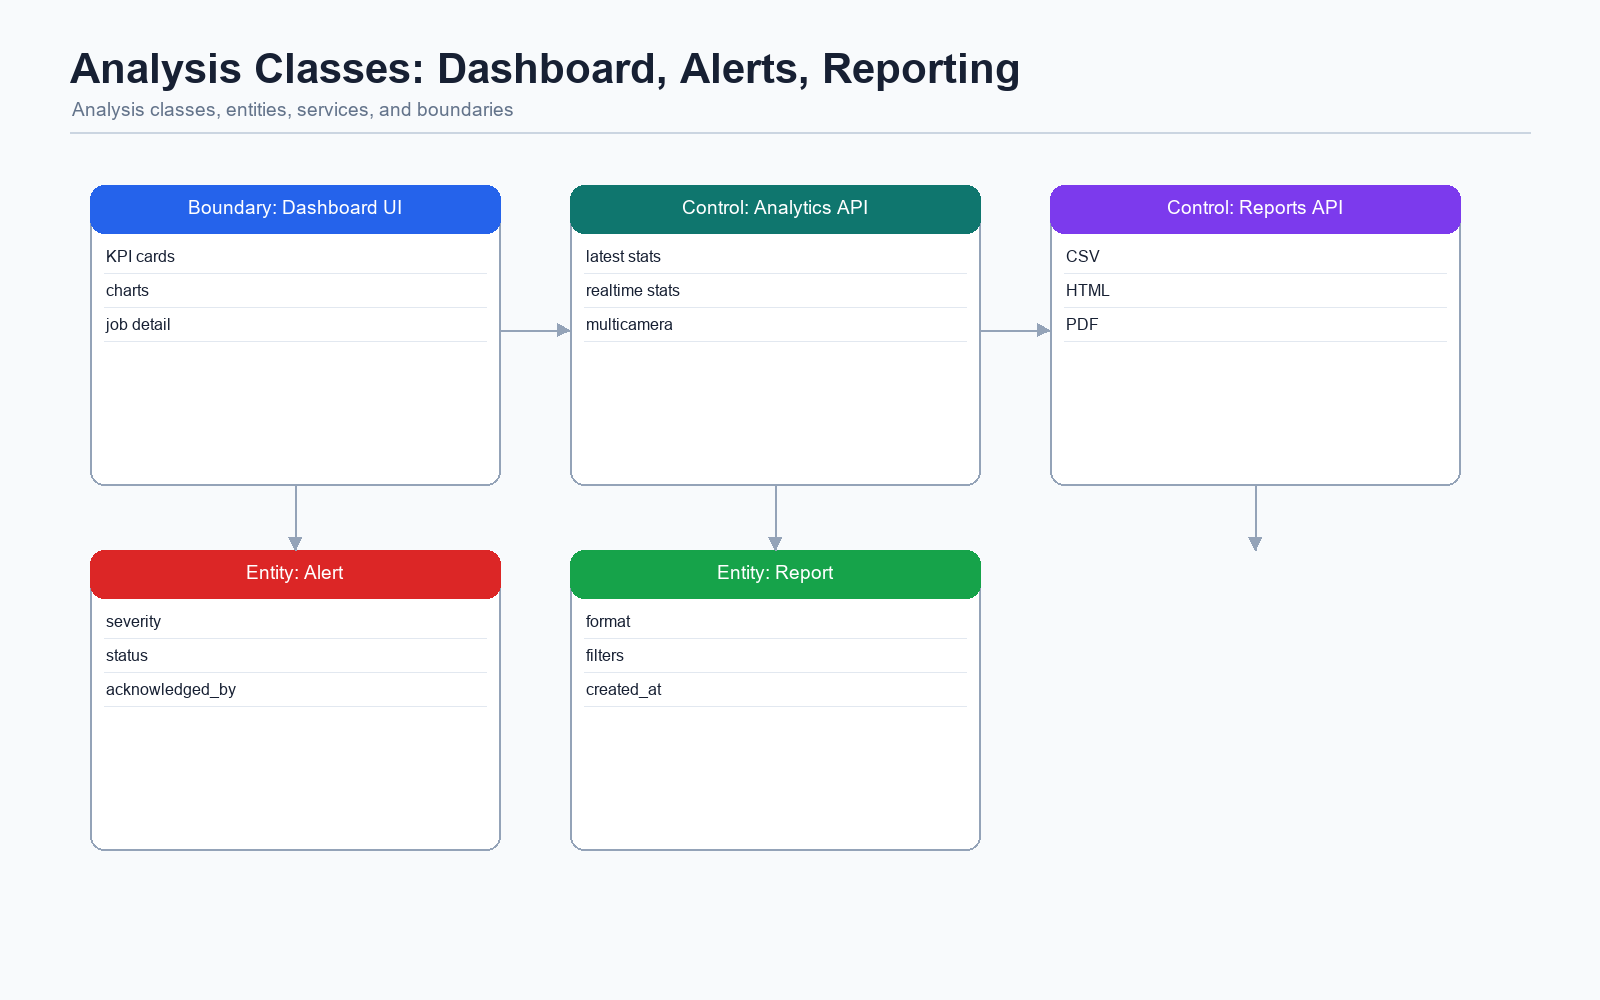
\includegraphics[width=\textwidth]{figures/analysis-class-dashboard-reporting.png}
    \caption{Analysis class decomposition for dashboard, alert monitoring, and reporting}
    \label{fig}
\end{figure}

\section{Sequence Diagrams}
\label{sec:sequence-diagrams}

Sequence diagrams describe how the main objects interact over time to complete important system operations. 
For this project, the most important workflows are login, user management, video upload and analysis job creation, zone configuration, pedestrian analysis, dashboard analytics retrieval, alert monitoring, and report export.

\begin{figure}[H]
    \centering
    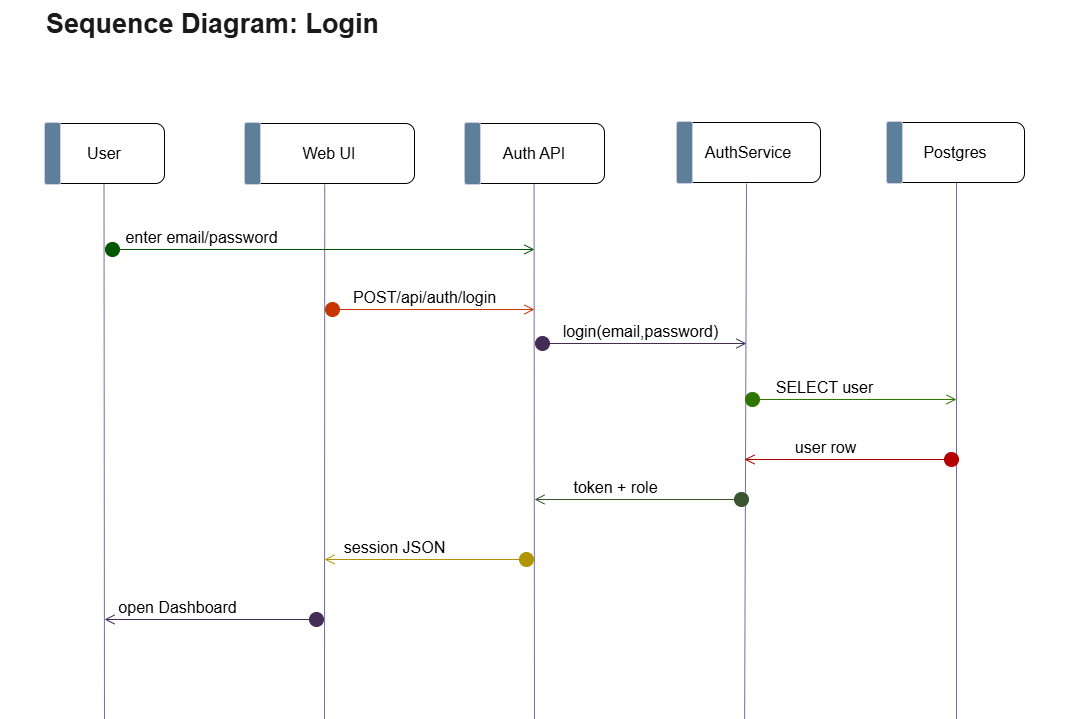
\includegraphics[width=\textwidth]{figures/Sequence-sequence-login.png}
    \caption{Sequence diagram for login}
    \label{fig}
\end{figure}

\begin{figure}[H]   
    \centering
    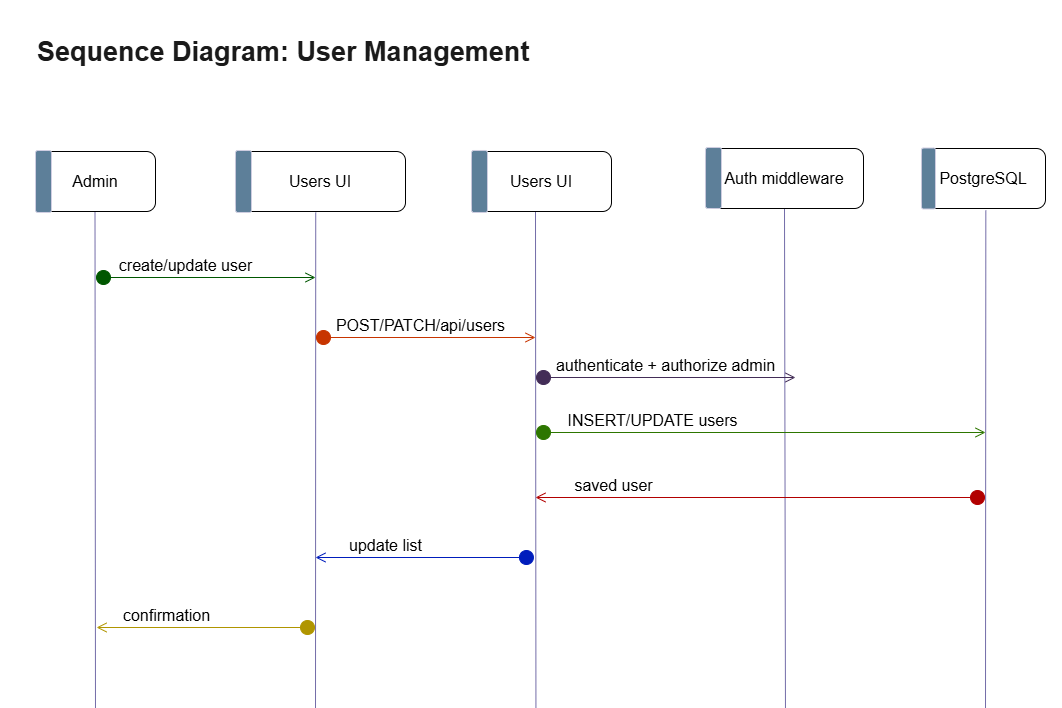
\includegraphics[width=\textwidth]{figures/Sequence-sequen-user-management.png}
    \caption{Sequence diagram for user management}
    \label{fig}
\end{figure}

\begin{figure}[H]
    \centering
    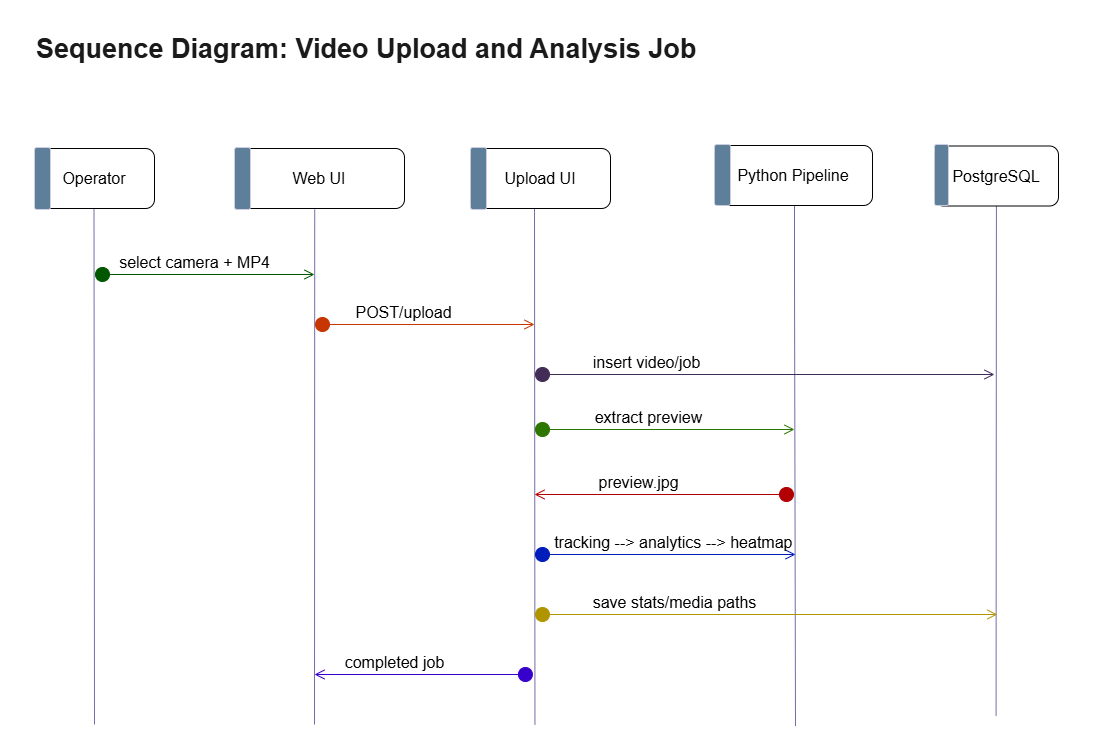
\includegraphics[width=\textwidth]{figures/Sequence-sequence-video-upload-analysis.png}
    \caption{Sequence diagram for analysis video upload}
    \label{fig}
\end{figure}

\begin{figure}[H]
    \centering
    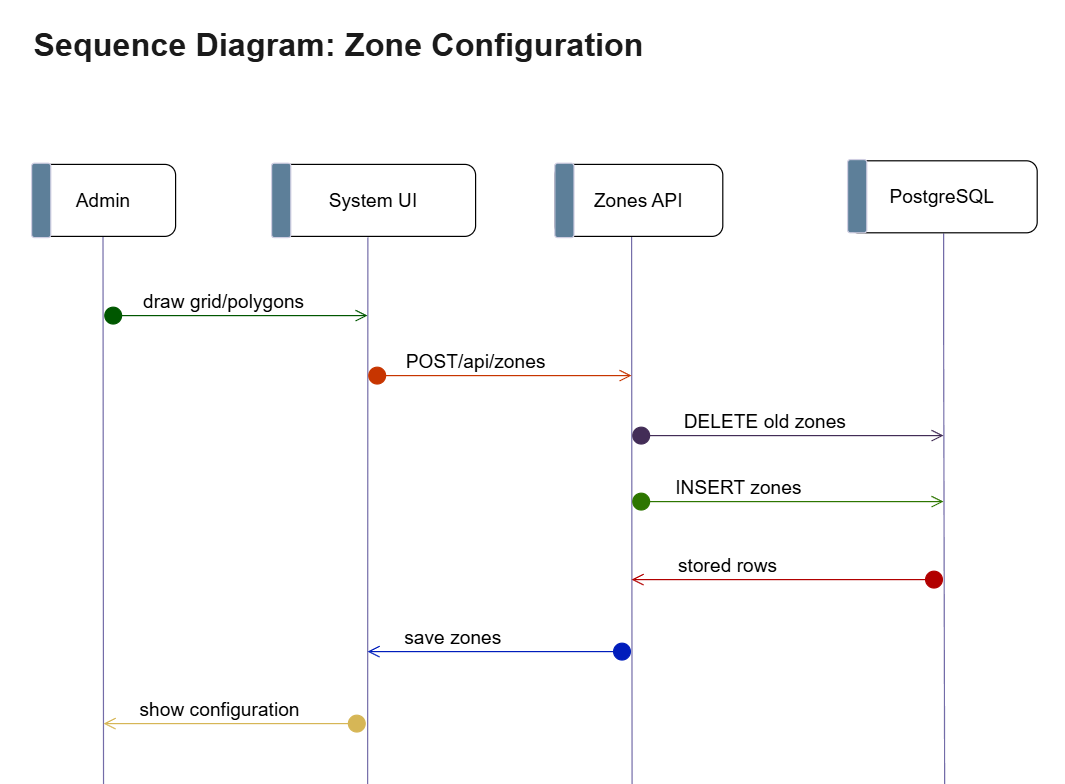
\includegraphics[width=\textwidth]{figures/Sequence-sequence-zone-configuration.png}
    \caption{Sequence diagram for zone configuration and threshold setup}
    \label{fig}
\end{figure}

\begin{figure}[H]
    \centering
    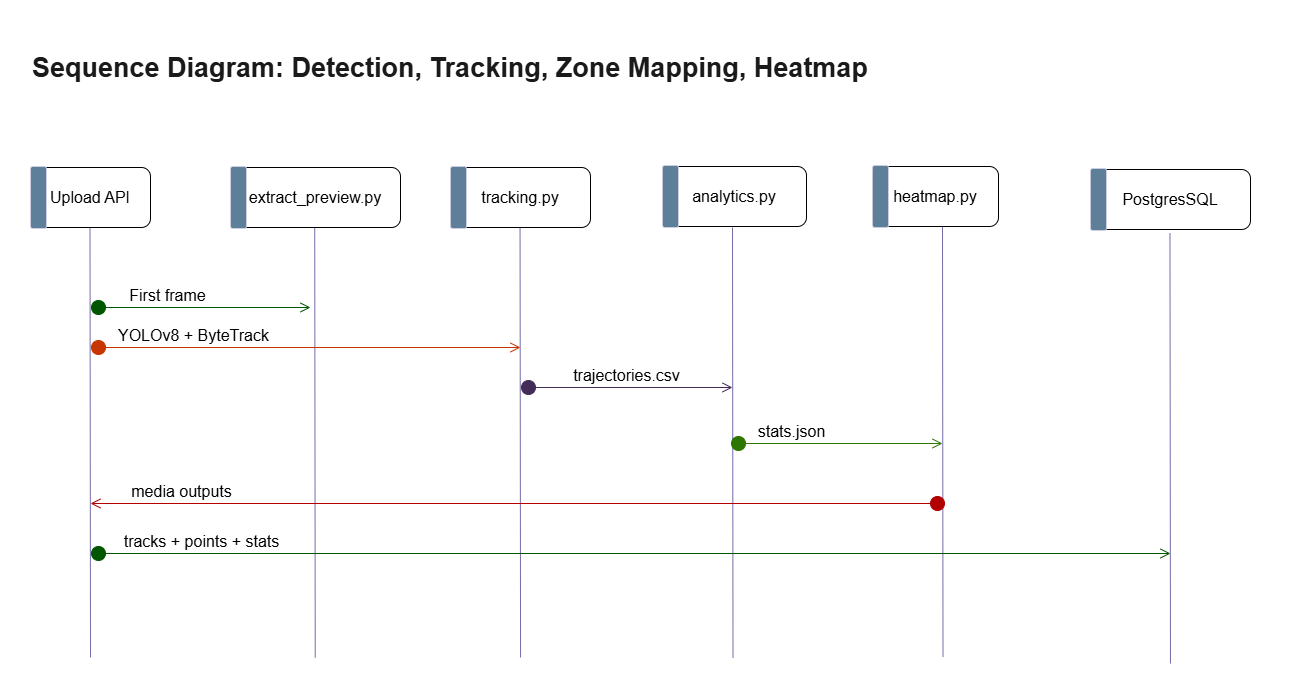
\includegraphics[width=\textwidth]{figures/Sequence-sequence-detection-tracking-heatmap.png}
    \caption{Sequence diagram for detection, tracking and create heatmap}
    \label{fig}
\end{figure}

\begin{figure}[H]
    \centering
    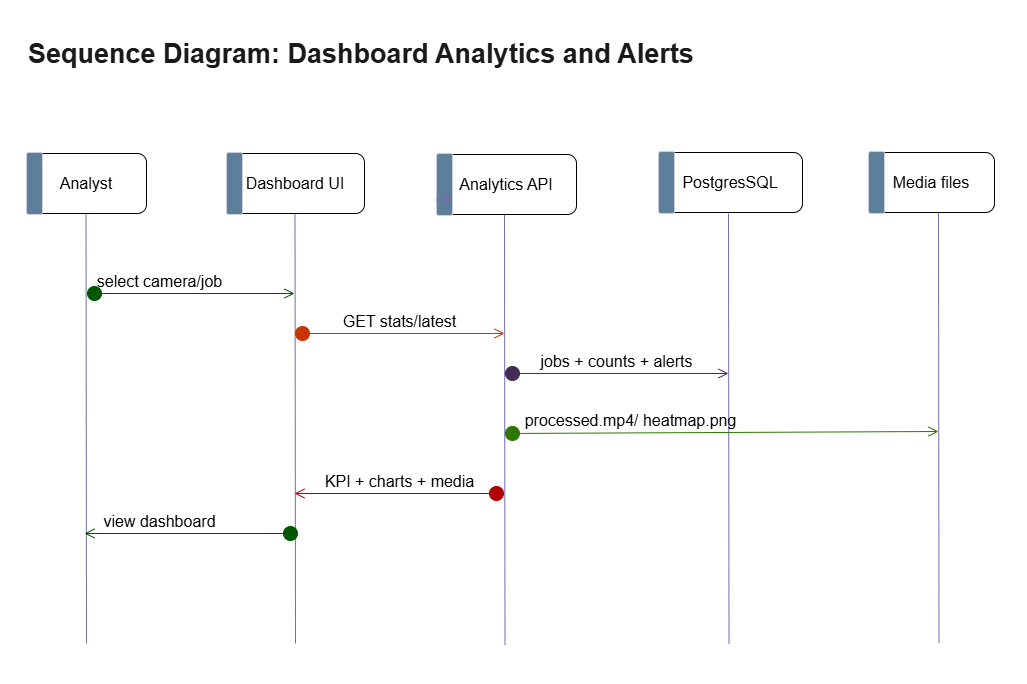
\includegraphics[width=\textwidth]{figures/Sequence-sequence-dashboard-alerts.png}
    \caption{Sequence diagram for dashboard analytics and alert retrieval}
    \label{fig}
\end{figure}

\begin{figure}[H]
    \centering
    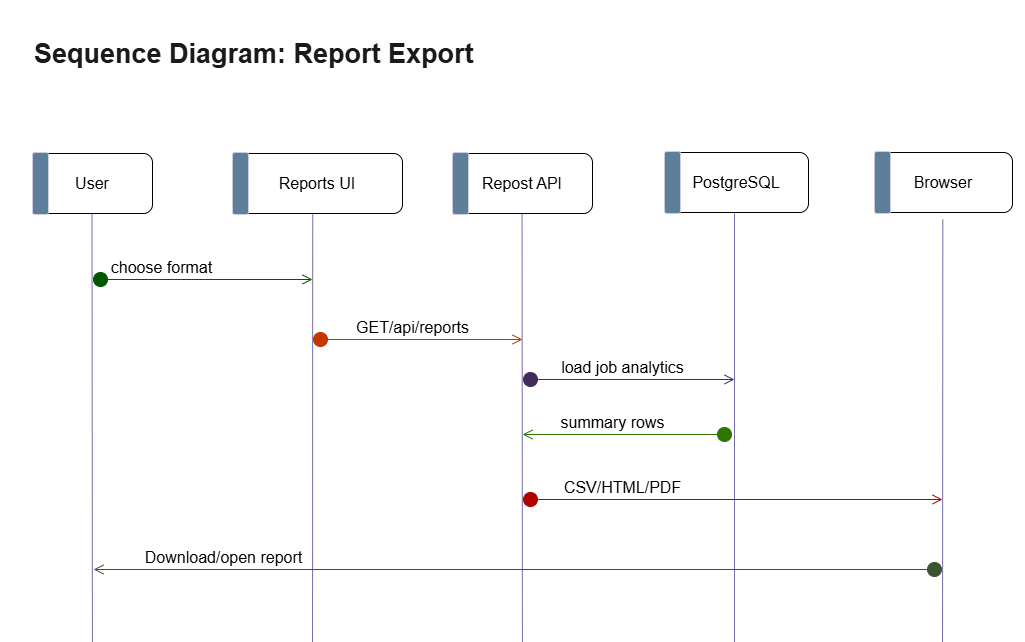
\includegraphics[width=\textwidth]{figures/Sequence-sequence-report-export.png}
    \caption{Sequence diagram for report export}
    \label{fig}
\end{figure}

\section{Analysis Class Diagram}
\label{sec:analysis-class-diagram}

The analysis class diagram shows the relationships between boundary classes, control classes, and entity classes.
In this system, user-facing pages interact with backend controller classes through REST APIs, while controller classes access or update persistent entity classes through the PostgreSQL database layer.
The computer vision processing logic is coordinated through the analysis job and pedestrian processing controllers.
The dashboard does not directly process raw video frames.
Instead, it reads already-computed analytics such as zone counts, transition flow, density scores, dwell times, alerts, processed video paths, preview image paths, heatmap image paths, and heatmap video paths.

\begin{figure}[H]
    \centering
    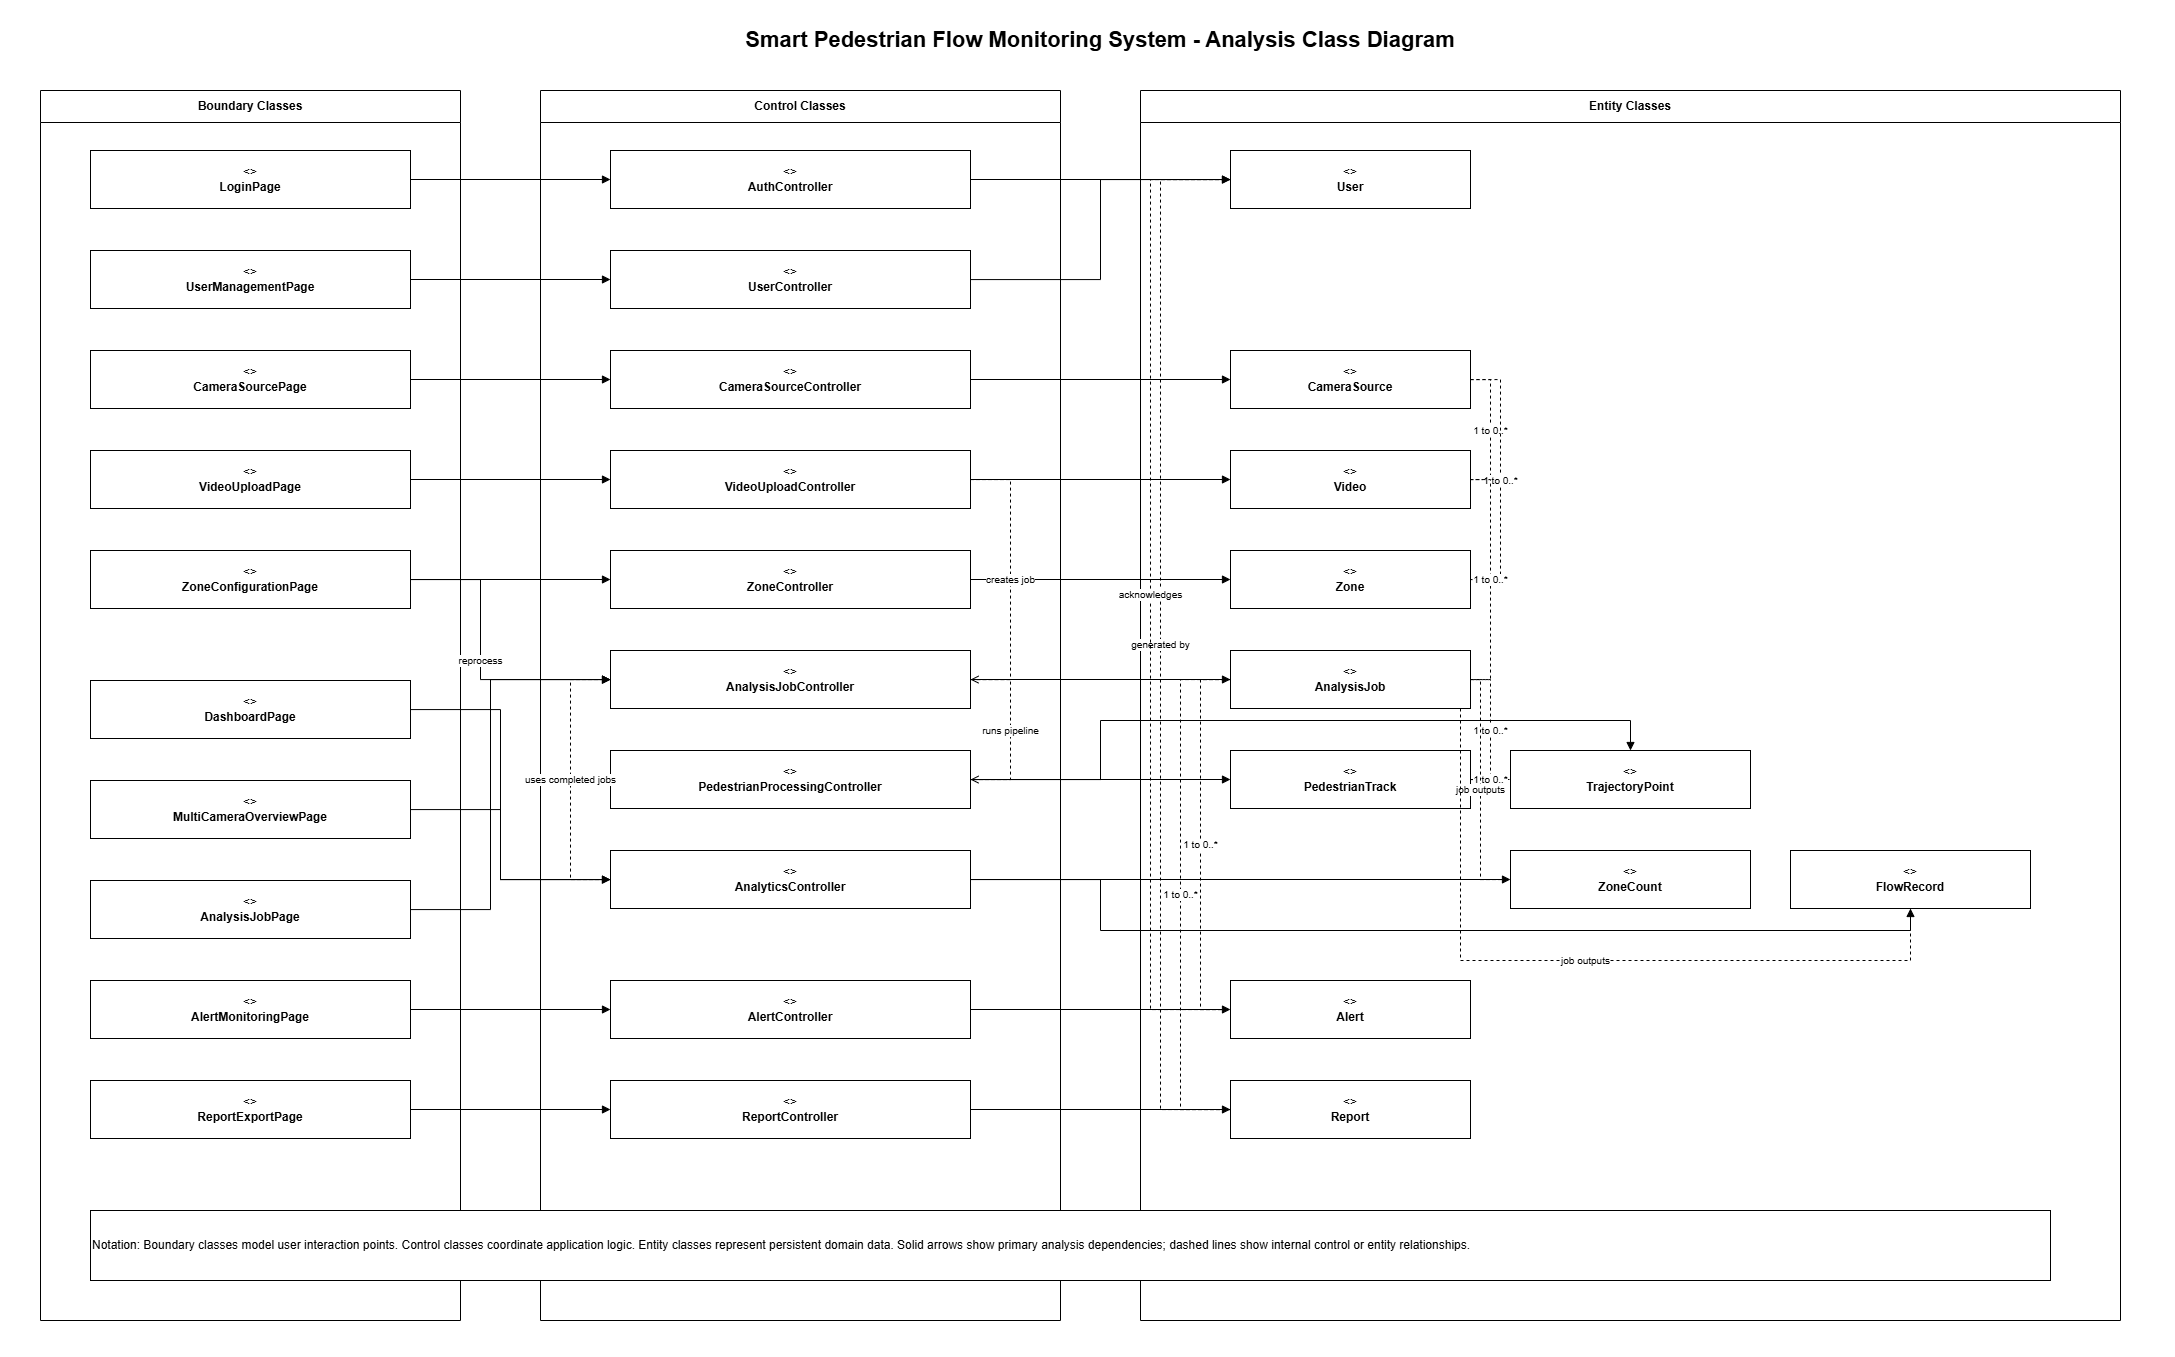
\includegraphics[width=\textwidth]{figures/analysis-class-diagram.png}
    \caption{Analysis class diagram of the Smart Pedestrian Flow Monitoring System}
    \label{fig}
\end{figure}

\section{Entity Relationship Diagram}
\label{sec:entity-relationship-diagram}

The Entity Relationship Diagram describes the main data entities required by the system and how they are related.
The implemented prototype uses PostgreSQL to store user accounts, camera source metadata, uploaded video metadata, zone configuration, analysis jobs, anonymous pedestrian tracks, trajectory points, zone counts, transition flow records, alerts, and report export history.
The design supports multiple logical camera sources, and each completed analysis job stores its own generated media paths so that dashboard and report views can load historical results without overwriting other camera outputs.

\subsection*{Identified Data Entities}

\begin{longtable}{|p{4.0cm}|p{9.8cm}|}
\hline
\rowcolor{HeaderBlue}
\textbf{Entity} & \textbf{Description} \\
\hline
User & Stores user account information, password hash, role, and account status. \\
\hline
Role & Defines the supported permission groups: admin, analyst, and staff. It is implemented as a constrained role field in the user record. \\
\hline
CameraSource & Stores logical camera source information such as name, location, description, and status. \\
\hline
Video & Stores uploaded video metadata such as file name, original file name, file path, camera source, status, upload time, and processed time. \\
\hline
Zone & Stores zone name, zone type, polygon or line coordinates, camera source, order position, and threshold value. \\
\hline
AnalysisJob & Stores processing status, aggregate analytics, generated media paths, start time, finish time, and error message for each video analysis execution. \\
\hline
HeatmapOutput & Represents generated heatmap media for an analysis job. It is implemented through the heatmap image path and heatmap video path stored in the analysis job record. \\
\hline
PedestrianTrack & Stores anonymous track information generated during detection and tracking. \\
\hline
TrajectoryPoint & Stores frame-level position points for each pedestrian track and the mapped zone name. \\
\hline
ZoneCount & Stores the number of pedestrians counted in each zone for an analysis job. \\
\hline
FlowRecord & Stores transition counts between zones for an analysis job. \\
\hline
Alert & Stores alerts generated when zone counts exceed configured thresholds and stores acknowledgement metadata. \\
\hline
Report & Stores report export metadata, including selected analysis job, selected camera source, generated user, format, filters, and creation time. \\
\hline
\end{longtable}

\subsection*{Entity Relationship Description}

\begin{enumerate}
    \item One role can be assigned to many users, while each user has exactly one role.
    \item One user can generate many report export records, while each report export record is generated by zero or one user if the account is later removed.
    \item One user can acknowledge many alerts, while each alert is acknowledged by zero or one user.
    \item One camera source can be associated with many uploaded videos.
    \item One camera source can have many configured zones.
    \item One camera source can have many analysis jobs, although the camera reference may become empty if the camera source is deleted.
    \item One video can be processed by one or more analysis jobs.
    \item One analysis job belongs to one video and optionally one camera source.
    \item One zone belongs to one camera source and stores one threshold value used for alert generation.
    \item One configured zone may be referenced by many zone count records and alert records through its zone name.
    \item One analysis job stores aggregate analytics such as total people, most crowded zone, popular path, zone counts, transition flow, timeline, dwell times, density scores, and congestion status.
    \item One analysis job can generate zero or one heatmap output artifact.
    \item One analysis job can generate many pedestrian tracks.
    \item One pedestrian track can contain many trajectory points.
    \item One trajectory point may be mapped to one zone name.
    \item One analysis job can generate many zone count records.
    \item One analysis job can generate many flow records representing transitions between zones.
    \item One analysis job can generate many alerts when threshold conditions are satisfied.
    \item One analysis job can be used to generate many exported reports.
\end{enumerate}

\begin{figure}[H]
    \centering
    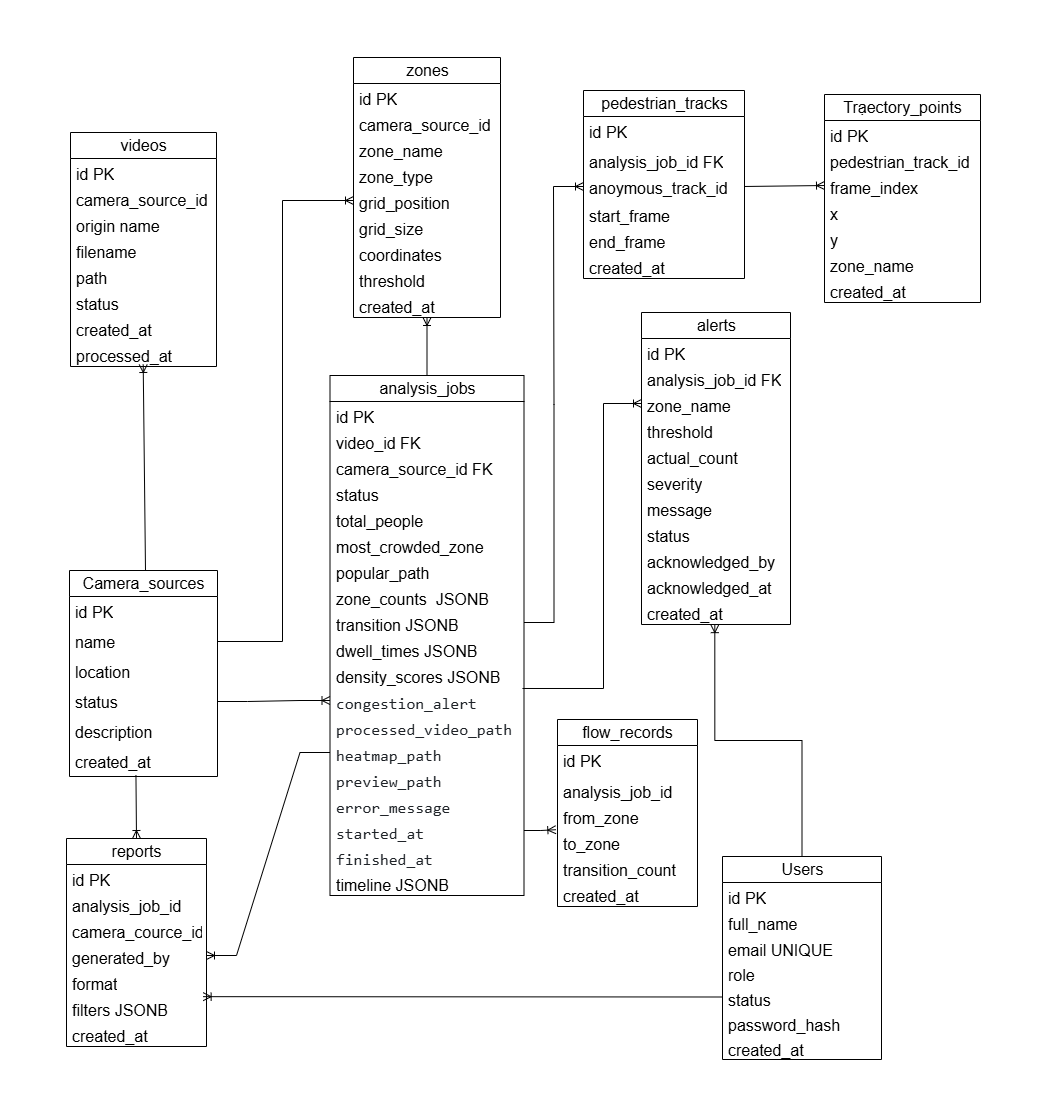
\includegraphics[width=\textwidth]{figures/erd (2).png}
    \caption{Entity Relationship Diagram of the Smart Pedestrian Flow Monitoring System}
    \label{fig}
\end{figure}
    
\section{Main Analysis Scenarios}
\label{sec:main-analysis-scenarios}

This section summarizes the main scenarios that connect the identified classes and entities with actual user operations.
These scenarios also clarify how the implemented offline video prototype demonstrates the core workflow of the larger pedestrian flow monitoring system.

\subsection*{Scenario 1: Login and Access Control}

A user opens the system and enters login credentials.
The backend validates the email and password against the stored user table.
If the credentials are valid and the account is active, the backend creates an in-memory session token and returns the token with the user's profile.
The frontend uses this token in later API requests.
The displayed functions depend on the user's role.

The supported roles are:

\begin{itemize}
    \item \textbf{Admin}: has all permissions, including user management, camera source management, video upload, zone configuration, reprocessing, dashboard access, alert monitoring, and report export.
    \item \textbf{Analyst}: can access analytics pages, job history, dashboard views, and report export features.
    \item \textbf{Staff}: can monitor alerts and operational overview pages, especially alert-related information.
\end{itemize}

If login fails, the system returns an error response and denies access to protected functions.

\subsection*{Scenario 2: User Management}

An administrator opens the user management page and views the list of registered users.
The administrator can create a new account, update a user's role, change account status, or update account information.
The system validates the input, hashes passwords before storage, persists the updated user information in PostgreSQL, and refreshes the user list.
Only administrators are allowed to manage user accounts.

\subsection*{Scenario 3: Camera Source Management}

An administrator opens the camera source page to create or manage logical camera sources.
A camera source represents a monitored location or logical video source, such as a lobby, corridor, or entrance camera.
The current implementation does not connect to a live stream URL.
Instead, camera sources are metadata records used to organize uploaded videos and analysis results by location.
Only administrators can create, update, or delete camera sources.
Other authenticated users can view available camera sources according to their dashboard permissions.

\subsection*{Scenario 4: Video Upload and Analysis Job Creation}

An administrator selects a camera source and uploads an offline video file.
The backend stores the uploaded file, creates a video metadata record, and creates a new analysis job with processing status.
The processing pipeline then generates a preview image, runs YOLO-based pedestrian detection, assigns temporary anonymous track IDs using ByteTrack-based tracking, computes analytics, generates heatmap image and heatmap video outputs, and stores the resulting media paths.
If processing succeeds, the analysis job is marked as completed.
If processing fails, the job is marked as failed and the error message is stored.

\subsection*{Scenario 5: Zone Configuration and Reprocessing}

An administrator opens the zone configuration page and defines monitoring zones on the video preview.
The current prototype supports manually drawn polygon zones and line zones.
Polygon zones are used for zone-level occupancy and density analysis.
Line zones are used for crossing-style analytics based on pedestrian trajectories.
Each zone has a name, type, normalized coordinates, display order, and threshold value.

After zones are saved, the frontend can request backend reprocessing for the latest uploaded video of the selected camera source.
This creates a new analysis job using the updated zone configuration.
As a result, dashboard statistics, alerts, transition flow, and reports reflect the latest zone setup.

\subsection*{Scenario 6: Pedestrian Analysis and Heatmap Generation}

The system processes the uploaded video through the Python computer vision pipeline.
First, it extracts a preview frame for zone configuration and display.
Then it detects pedestrians using a YOLO-based detector and assigns anonymous temporary track IDs using ByteTrack-based tracking.
The tracking output is saved as trajectory data and persisted into PostgreSQL as pedestrian tracks and trajectory points.
Based on these trajectory points and configured zones, the system computes total people, zone counts, transition flow, timeline statistics, dwell time estimates, density scores, congestion status, and generated alerts.
A heatmap image and a heatmap video are also generated as visualizations of frequent pedestrian presence and movement.

\subsection*{Scenario 7: Dashboard Analytics and Realtime Video-Window Statistics}

After an analysis job is completed, the user opens the dashboard.
The dashboard retrieves stored analytics results from the backend, including total people, most crowded zone, popular path, zone counts, transition flow, heatmap image path, heatmap video path, processed video path, preview image path, density scores, dwell times, and congestion status.

While the processed video is playing, the frontend can call a realtime statistics endpoint with the current video time.
The backend converts the video time to a frame index and reads trajectory points within a nearby frame window.
It then returns approximate current people count, current most crowded zone, zone counts, and congestion status for that moment of the video.
This gives the dashboard a realtime-like behavior while still using an offline processed video.

\subsection*{Scenario 8: Alert Monitoring}

The alert monitoring function compares computed zone counts with configured zone thresholds.
If a zone count exceeds its threshold, the system creates an alert record with severity, actual count, threshold, message, status, and creation time.
Users can view alerts for a selected camera source.
Staff users mainly use this feature to monitor operational alerts.
An alert can be acknowledged, and the system stores the acknowledging user and acknowledgement time.

\subsection*{Scenario 9: Job History and Multi-Camera Overview}

Users can view historical analysis jobs and inspect job details.
The job detail view includes camera metadata, video metadata, job status, output media paths, zone count rows, flow rows, alerts, and track summary.
The multi-camera overview shows all logical camera sources with the latest completed analysis result and processed video for each camera.
This allows users to compare different locations and open the latest job for a selected camera source.

\subsection*{Scenario 10: Report Export}

An administrator or analyst selects a completed analysis job and exports the result.
The backend gathers relevant analytics, including total people, most crowded zone, popular path, zone counts, transitions, dwell times, density scores, timeline data, congestion status, and finish time.
The system can export the result as a CSV file, render a printable HTML report, or generate a simple backend PDF report.
Each export request is stored as report metadata in PostgreSQL for later reference.

% =====================================================
% CHAPTER 4
% =====================================================
\chapter{SYSTEM DESIGN}

\section{Architecture Design}

\subsection{Selected Architecture}

The Smart Pedestrian Flow Monitoring and Analytics System is designed as a modular client--server application combined with a dedicated computer vision processing pipeline. The architecture separates user interface logic, backend services, video analytics processing, and persistent storage in order to simplify maintenance, improve scalability, and support future extension to multiple cameras or realtime processing.



The current implementation mainly focuses on an offline video analysis workflow using uploaded MP4 videos instead of realtime camera streams. This approach is suitable for the project scope and available hardware resources while still demonstrating the core pedestrian analytics functionalities.

The high-level architecture contains the following layers:

\begin{itemize}

    \item \textbf{Frontend/UI layer}: provides the web-based user interface for login, account management, camera management, zone configuration, dashboard visualization, heatmap display, transition-flow analysis, alert monitoring, job history, and report export. The frontend is implemented using HTML, CSS, JavaScript, and Bootstrap-based components.

    \item \textbf{Backend/API layer}: provides REST-style backend APIs and business logic for authentication, authorization, account management, job management, zone management, analytics retrieval, alert handling, and report export. The backend is implemented using Node.js with the Express.js framework.

    \item \textbf{Computer Vision Processing layer}: receives uploaded MP4 videos and performs pedestrian detection, tracking, trajectory extraction, zone-event mapping, and heatmap generation. The processing pipeline is implemented in Python using OpenCV and Ultralytics YOLO for pedestrian detection together with multi-object tracking algorithms.

    \item \textbf{Analytics layer}: computes pedestrian statistics such as zone counts, line-crossing counts, dwell time, density estimation, transition flow between zones, crowded-area alerts, timeline statistics, and summary analytics used by the dashboard and reports.

    \item \textbf{Database/File storage layer}: stores user accounts, uploaded videos, camera metadata, zone configurations, analysis jobs, trajectory records, analytics results, alerts, and exported report metadata. The system uses PostgreSQL as the primary relational database and local file storage for videos, generated heatmap images, generated heatmap videos, preview frames, and exported reports.

\end{itemize}

The modular separation between the frontend, backend, analytics pipeline, and storage components allows the system to support future improvements such as realtime camera streaming, distributed processing, additional analytics modules, or integration with external monitoring platforms.


\subsection{Main Components}

\begin{longtable}{|p{4cm}|p{10cm}|}
\hline
\rowcolor{HeaderBlue}
\textbf{Component} & \textbf{Responsibility} \\
\hline

Authentication module & Handles login, session token creation, password verification, logout, and role-based access control for \texttt{admin}, \texttt{staff}, and \texttt{analyst}. \\
\hline

User management module & Allows administrators to create user accounts, update roles, and activate or deactivate accounts. \\
\hline

Camera/source management module & Manages logical camera sources, camera metadata, status, and uploaded MP4 videos associated with each camera. \\
\hline

Zone configuration module & Allows authorized users to define polygon or line zones on video previews and configure density thresholds for monitored zones. \\
\hline

Analysis job module & Creates, runs, tracks, and reprocesses video analysis jobs, including job status, input video, output media, and processing results. \\
\hline

Detection module & Detects pedestrians from video frames using the YOLO-based computer vision model implemented in the Python processing pipeline. \\
\hline

Tracking module & Assigns anonymous pedestrian track IDs across frames and maintains movement trajectories without storing personal identity information. \\
\hline

Zone mapping module & Maps detected pedestrian positions and trajectories to configured zones and line-crossing regions. \\
\hline

Analytics module & Computes zone counts, line-crossing statistics, density scores, dwell time, movement timeline, heatmap data, and transition flows. \\
\hline

Alert module & Generates congestion or overcrowding alerts when zone density values exceed configured thresholds and supports alert acknowledgement. \\
\hline

Dashboard and visualization module & Displays KPI cards, processed video, camera overview, zone statistics, heatmap video, movement timeline, transition flow, alerts, and job results. \\
\hline

History module & Stores and displays previous analysis jobs, job details, processed media paths, zone counts, transition records, and track summaries. \\
\hline

Report module & Exports analytics results as CSV, printable HTML reports, and backend-generated PDF reports; also maintains generated report history. \\
\hline

Storage module & Stores users, cameras, zones, jobs, analytics results, alerts, and report metadata in PostgreSQL, while videos, previews, heatmap images, heatmap videos, and reports are stored as local files. \\
\hline

\end{longtable}

\section{Database Design}

{\small
\subsection{Table: users}
\begin{longtable}{|p{3.2cm}|p{3cm}|p{4.2cm}|p{4.5cm}|}
\hline
\rowcolor{HeaderBlue}
\textbf{Field} & \textbf{Type} & \textbf{Constraint} & \textbf{Note} \\
\hline
id & SERIAL & Primary key & User ID \\
\hline
full\_name & VARCHAR(120) & Not null & Full name \\
\hline
email & VARCHAR(160) & Unique, not null & Login email \\
\hline
password\_hash & TEXT & Not null & Hashed password \\
\hline
role & VARCHAR(30) & Not null, check constraint & \texttt{admin}, \texttt{analyst}, \texttt{staff} \\
\hline
status & VARCHAR(20) & Not null, default \texttt{active} & Account status \\
\hline
created\_at & TIMESTAMP & Not null, default \texttt{NOW()} & Created time \\
\hline
\end{longtable}

\subsection{Table: camera\_sources}
\begin{longtable}{|p{3.2cm}|p{3cm}|p{4.2cm}|p{4.5cm}|}
\hline
\rowcolor{HeaderBlue}
\textbf{Field} & \textbf{Type} & \textbf{Constraint} & \textbf{Note} \\
\hline
id & SERIAL & Primary key & Camera source ID \\
\hline
name & VARCHAR(120) & Not null & Camera/source name \\
\hline
location & VARCHAR(160) & Nullable & Camera location \\
\hline
description & TEXT & Nullable & Camera description \\
\hline
status & VARCHAR(30) & Not null, default \texttt{active} & Camera status \\
\hline
created\_at & TIMESTAMP & Not null, default \texttt{NOW()} & Created time \\
\hline
\end{longtable}

\subsection{Table: videos}
\begin{longtable}{|p{3.2cm}|p{3cm}|p{4.2cm}|p{4.5cm}|}
\hline
\rowcolor{HeaderBlue}
\textbf{Field} & \textbf{Type} & \textbf{Constraint} & \textbf{Note} \\
\hline
id & SERIAL & Primary key & Video ID \\
\hline
camera\_source\_id & INTEGER & Foreign key, nullable & References \texttt{camera\_sources.id} \\
\hline
filename & TEXT & Not null & Stored filename \\
\hline
original\_name & TEXT & Nullable & Original uploaded filename \\
\hline
path & TEXT & Not null & Storage path \\
\hline
status & VARCHAR(30) & Not null, default \texttt{uploaded} & Video status \\
\hline
created\_at & TIMESTAMP & Not null, default \texttt{NOW()} & Upload time \\
\hline
processed\_at & TIMESTAMP & Nullable & Processing completed time \\
\hline
\end{longtable}

\subsection{Table: zones}
\begin{longtable}{|p{3.2cm}|p{3cm}|p{4.2cm}|p{4.5cm}|}
\hline
\rowcolor{HeaderBlue}
\textbf{Field} & \textbf{Type} & \textbf{Constraint} & \textbf{Note} \\
\hline
id & SERIAL & Primary key & Zone ID \\
\hline
camera\_source\_id & INTEGER & Foreign key, cascade delete & References \texttt{camera\_sources.id} \\
\hline
zone\_name & VARCHAR(120) & Not null & Zone name \\
\hline
zone\_type & VARCHAR(60) & Default \texttt{monitoring} & Zone type \\
\hline
grid\_position & INTEGER & Not null & Zone order/index \\
\hline
grid\_size & INTEGER & Not null & Grid size metadata \\
\hline
coordinates & JSONB & Default empty array & Polygon or line geometry \\
\hline
threshold & INTEGER & Not null, default 10 & Alert threshold \\
\hline
created\_at & TIMESTAMP & Not null, default \texttt{NOW()} & Created time \\
\hline
\end{longtable}

\subsection{Table: analysis\_jobs}
\begin{longtable}{|p{3.6cm}|p{3cm}|p{4.2cm}|p{4.5cm}|}
\hline
\rowcolor{HeaderBlue}
\textbf{Field} & \textbf{Type} & \textbf{Constraint} & \textbf{Note} \\
\hline
id & SERIAL & Primary key & Analysis job ID \\
\hline
video\_id & INTEGER & Foreign key, cascade delete & References \texttt{videos.id} \\
\hline
camera\_source\_id & INTEGER & Foreign key, nullable & References \texttt{camera\_sources.id} \\
\hline
status & VARCHAR(30) & Not null, default \texttt{queued} & Job status \\
\hline
total\_people & INTEGER & Default 0 & Total detected people \\
\hline
most\_crowded\_zone & VARCHAR(120) & Nullable & Peak zone name \\
\hline
popular\_path & VARCHAR(240) & Nullable & Most frequent movement path \\
\hline
zone\_counts & JSONB & Default empty object & People count per zone \\
\hline
transitions & JSONB & Default empty object & Zone transition summary \\
\hline
timeline & JSONB & Default empty array & Time-based people count \\
\hline
dwell\_times & JSONB & Default empty object & Dwell time per zone \\
\hline
density\_scores & JSONB & Default empty object & Density score per zone \\
\hline
congestion\_alert & TEXT & Default \texttt{Normal} & Overall congestion status \\
\hline
processed\_video\_path & TEXT & Nullable & Processed video path \\
\hline
heatmap\_path & TEXT & Nullable & Heatmap image path \\
\hline
heatmap\_video\_path & TEXT & Nullable & Heatmap video path \\
\hline
preview\_path & TEXT & Nullable & Preview image path \\
\hline
error\_message & TEXT & Nullable & Failure reason \\
\hline
started\_at & TIMESTAMP & Nullable & Processing start time \\
\hline
finished\_at & TIMESTAMP & Nullable & Processing finish time \\
\hline
created\_at & TIMESTAMP & Not null, default \texttt{NOW()} & Job created time \\
\hline
\end{longtable}
}

\section{Detailed Package Design}
\begin{figure}[H]
    \centering
    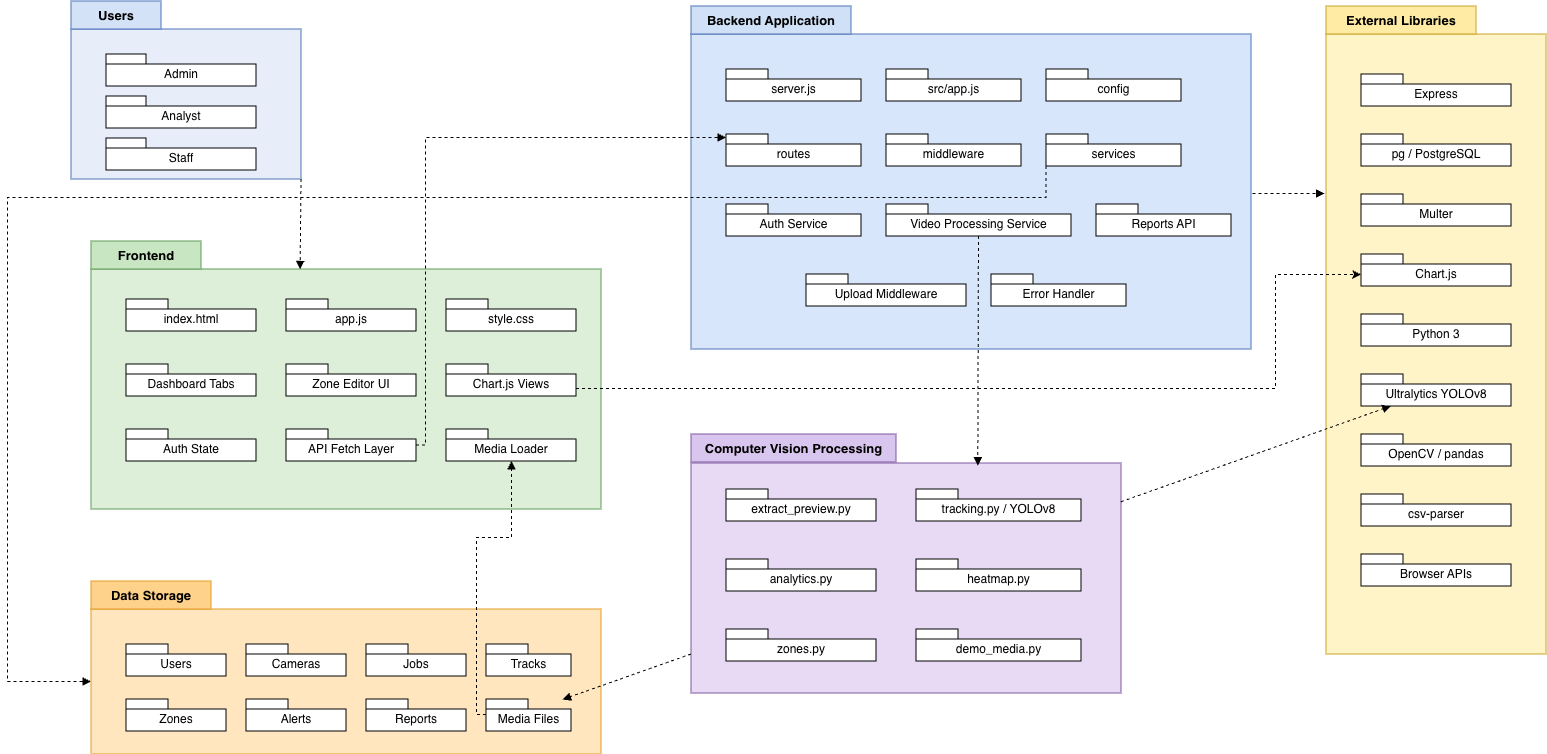
\includegraphics[width=\textwidth]{figures/overall-package-design.png}
    \caption{Overall package design}
    \label{fig:overall-package-design}
\end{figure}
\subsection{Frontend Package Design}

The frontend of the system is implemented as a static web dashboard and is served directly by the Express backend. The project does not use a separate frontend framework such as React or Vue. All frontend files are located in the \texttt{backend/public} directory.

\begin{itemize}
    \item \textbf{index.html}: defines the main user interface of the system, including login and registration screens, sidebar navigation, camera source management, dashboard, analytics, multi-camera overview, job history, alerts, reports, user management, and system configuration pages.
    
    \item \textbf{app.js}: implements frontend behavior such as authentication, role-based interface control, tab switching, REST API calls, camera selection, video upload, dashboard refresh, multi-camera monitoring, alert acknowledgement, report generation, job history viewing, and zone drawing/configuration.
    
    \item \textbf{style.css}: defines the visual layout and responsive design of the dashboard, including sidebar, topbar, cards, panels, forms, tables, video preview area, heatmap video display, zone editor, and modal components.
    
    \item \textbf{External libraries}: the frontend uses Chart.js to render analytics charts such as zone count charts and timeline charts.
\end{itemize}

\subsection{Backend Package Design}

The backend is implemented using Node.js and Express. It provides REST APIs, serves the static frontend, manages authentication and authorization, stores data in PostgreSQL, handles video uploads, and coordinates the Python-based computer vision pipeline.

The backend source code is currently organized under the \texttt{backend/src} directory, while \texttt{backend/server.js} remains the stable runtime entry point used by \texttt{npm start}.

\begin{itemize}
    \item \textbf{backend/server.js}: application startup file. It initializes the PostgreSQL database, seeds default users, creates the Express application, and starts the HTTP server.
    
    \item \textbf{backend/src/app.js}: creates and configures the Express application. It registers middleware, serves static frontend files from \texttt{backend/public}, mounts API routes, and attaches the global error handler.
    
    \item \textbf{backend/src/routes}: contains HTTP route modules.
    \begin{itemize}
        \item \texttt{auth.js}: login, registration, session validation, and user management APIs.
        \item \texttt{cameras.js}: camera source creation, listing, update, status change, and deletion APIs.
        \item \texttt{videos.js}: video upload and video reprocessing APIs.
        \item \texttt{zones.js}: zone configuration save and load APIs.
        \item \texttt{analytics.js}: dashboard statistics, realtime statistics, flow records, alerts, analysis jobs, and multi-camera overview APIs.
        \item \texttt{reports.js}: report export, print/PDF view, and report history APIs.
        \item \texttt{demo.js}: demo data and demo media generation API.
    \end{itemize}
    
    \item \textbf{backend/src/services}: contains reusable backend logic.
    \begin{itemize}
        \item \texttt{authService.js}: password hashing, login validation, default user seeding, JWT-like session authentication, and role-based authorization middleware.
        \item \texttt{VideoProcessingService.js}: coordinates the video processing workflow by calling Python scripts, generating preview, processed video, heatmap image, and heatmap video outputs, reading trajectory data, saving analysis jobs, alerts, zone counts, flow records, and trajectory points to PostgreSQL.
        \item \texttt{analyticsService.js}: provides analytics retrieval logic.
        \item \texttt{videoService.js}: provides video creation and processed-status update logic.
        \item \texttt{zoneService.js}: provides zone save, load, and delete logic.
    \end{itemize}
    
    \item \textbf{backend/src/config}: contains backend configuration.
    \begin{itemize}
        \item \texttt{db.js}: PostgreSQL connection pool and database initialization.
        \item \texttt{paths.js}: centralized runtime path definitions for uploads, outputs, public files, and context files.
        \item \texttt{schema.sql}: database schema definition for users, camera sources, videos, zones, analysis jobs, pedestrian tracks, trajectory points, flow records, zone counts, alerts, and reports.
    \end{itemize}
    
    \item \textbf{backend/src/middleware}: contains Express middleware.
    \begin{itemize}
        \item \texttt{uploadMiddleware.js}: handles video upload storage using Multer.
        \item \texttt{errorHandler.js}: returns consistent JSON error responses.
    \end{itemize}
    
    \item \textbf{backend/uploads}: stores uploaded raw video files at runtime.
    
    \item \textbf{backend/outputs}: stores runtime metadata such as current context and zone configuration files.
    
    \item \textbf{backend/public/media/jobs}: stores generated media for each analysis job, including preview images, processed videos, heatmap images, heatmap videos, trajectory CSV files, and statistics JSON files.
\end{itemize}

\subsection{Computer Vision Processing Package Design}

The computer vision processing layer is implemented in Python and located in the \texttt{ai\_services} directory. The Node.js backend invokes these scripts through \texttt{child\_process.execFile} inside \texttt{VideoProcessingService.js}.

\begin{itemize}
    \item \textbf{extract\_preview.py}: extracts a preview frame from the uploaded video so users can configure monitoring zones visually.
    
    \item \textbf{tracking.py}: detects and tracks pedestrians in the uploaded video. The current pipeline uses YOLOv8 through the Ultralytics library and assigns anonymous track IDs to detected pedestrians.
    
    \item \textbf{analytics.py}: reads trajectory CSV data and computes analytics such as total people, zone counts, transitions, timeline data, dwell time, popular path, and congestion status.
    
    \item \textbf{heatmap.py}: generates a heatmap image and a heatmap video from pedestrian trajectory points.
    
    \item \textbf{zones.py}: loads and normalizes zone configuration, maps tracked points to configured zones, and supports grid-based or polygon-based zone geometry.
    
    \item \textbf{demo\_media.py}: generates demo media used by the demo data workflow.
    
    \item \textbf{Runtime outputs}: each processing job can generate a preview image, processed video, heatmap image, heatmap video, trajectory CSV file, and statistics JSON file. These outputs are stored under \texttt{backend/public/media/jobs/<jobId>} and referenced by records in PostgreSQL.
\end{itemize}

\section{Detailed Class Design}

Although the backend is implemented mainly with JavaScript modules instead of a strict object-oriented class hierarchy, the main domain entities and modules can be described as follows.

\begin{longtable}{|p{4cm}|p{5cm}|p{5cm}|}
\hline
\rowcolor{HeaderBlue}
\textbf{Entity/Module} & \textbf{Main data} & \textbf{Main operations} \\
\hline
User & id, fullName, email, passwordHash, role, status, createdAt & login(), hashPassword(), authenticate(), authorize(), seedDefaultUsers() \\
\hline
CameraSource & id, name, location, description, status, createdAt & createCamera(), updateCamera(), toggleStatus(), deleteCamera(), listCameras() \\
\hline
Video & id, cameraSourceId, filename, originalName, path, status, createdAt, processedAt & uploadVideo(), createVideo(), markProcessed(), reprocessVideo() \\
\hline
Zone & id, cameraSourceId, zoneName, zoneType, gridPosition, gridSize, coordinates, threshold & saveZones(), getZones(), deleteZones(), normalizeGeometry(), getZone() \\
\hline
AnalysisJob & id, videoId, cameraSourceId, status, totalPeople, zoneCounts, transitions, timeline, dwellTimes, densityScores, mediaPaths & processVideo(), saveStatsToJob(), getAnalysisJobs(), getJobDetail() \\
\hline
PedestrianTrack & id, analysisJobId, anonymousTrackId, startFrame, endFrame & persistTrajectoryPoints(), groupTrajectoryByPerson() \\
\hline
TrajectoryPoint & id, pedestrianTrackId, frameIndex, x, y, zoneName & createTrajectoryPoint(), assignZone() \\
\hline
Alert & id, analysisJobId, zoneName, threshold, actualCount, severity, message, status & createThresholdAlert(), listAlerts(), acknowledgeAlert() \\
\hline
FlowRecord & id, analysisJobId, fromZone, toZone, transitionCount & computeTransitions(), saveFlowRecord(), listFlowRecords() \\
\hline
Report & id, analysisJobId, cameraSourceId, generatedBy, format, filters, createdAt & exportReport(), printReport(), generatePdfView(), listReports() \\
\hline
VideoProcessingService & pool, pythonBin, runtimePaths, mediaPaths & runPython(), getLatestZones(), writeRuntimeZonesFile(), processVideo(), persistTrajectoryPoints(), saveStatsToJob(), copyLatestMedia() \\
\hline
\end{longtable}

\section{Detailed Class Diagram}

\begin{figure}[H]
    \centering
    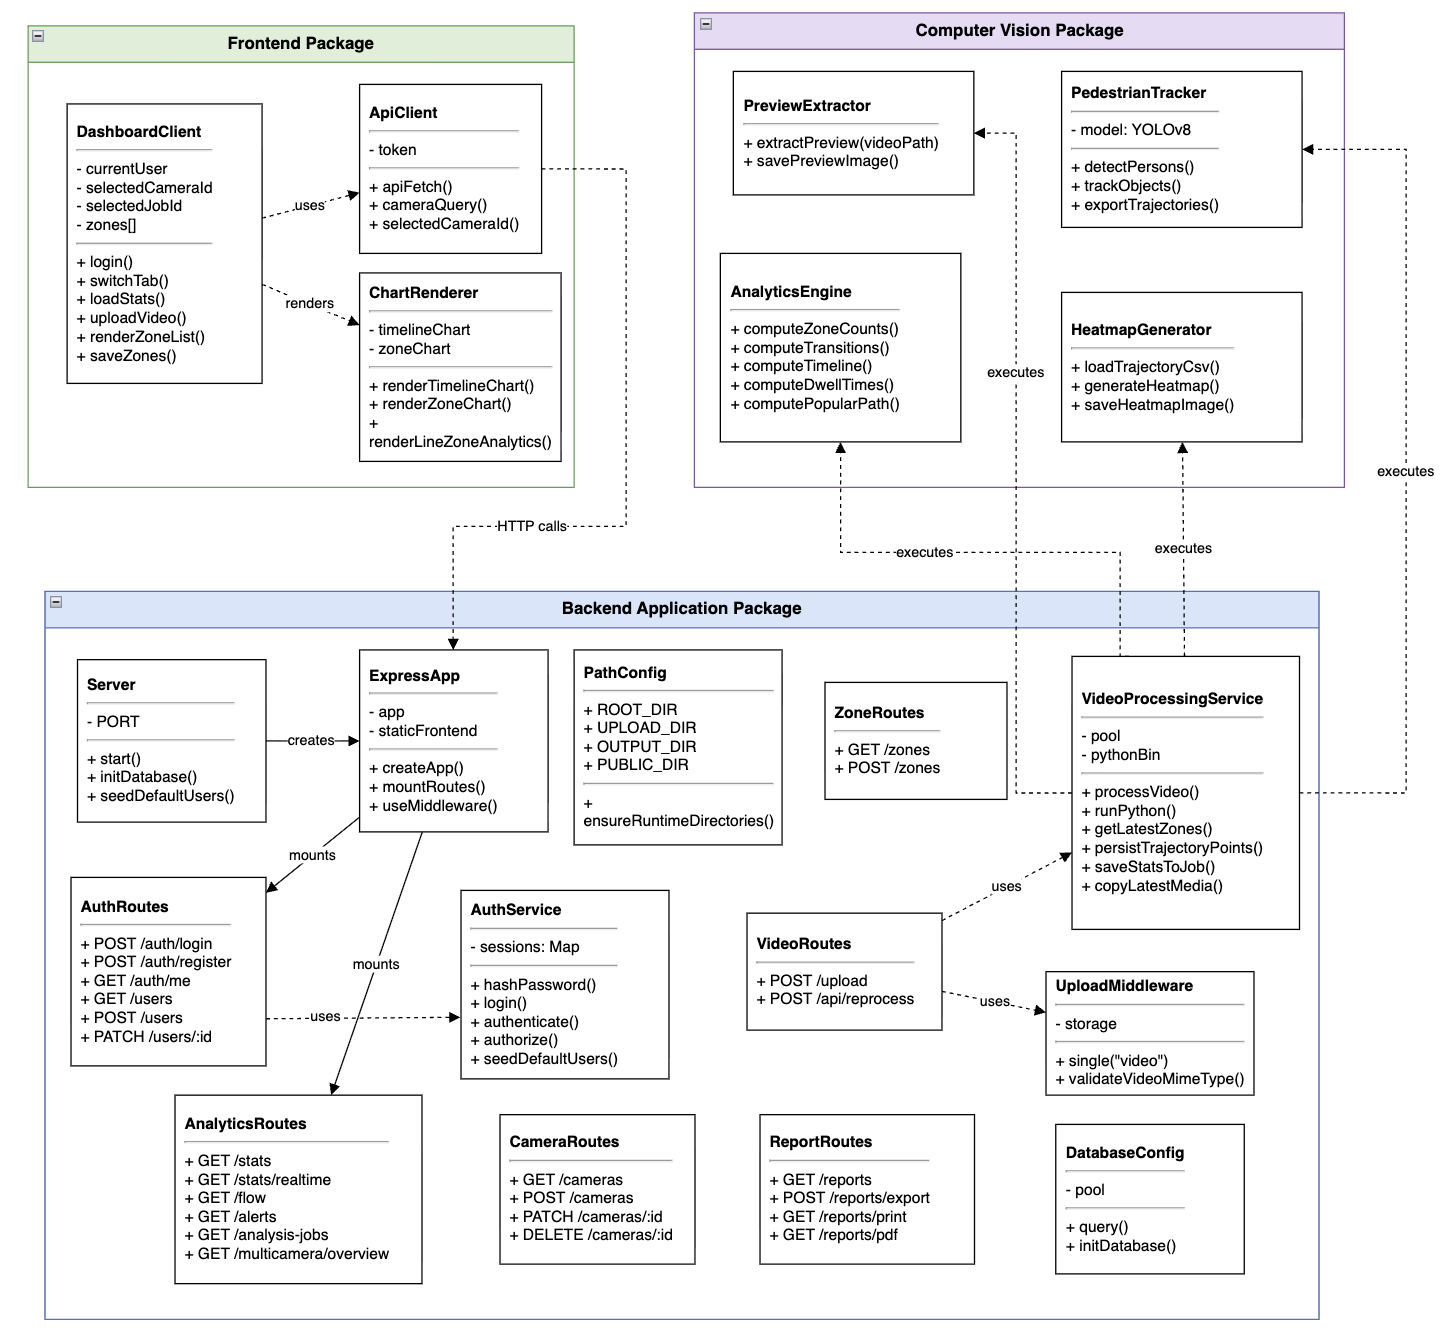
\includegraphics[width=\textwidth]{figures/detailed-class-diagram.png}
    \caption{Detailed class diagram}
    \label{fig:detailed-class-diagram}
\end{figure}

\section{Interface Design}
The system interface is designed as a single-page dashboard application. Users log in first, then interact with the system through the sidebar menu. The main interface contains a persistent sidebar, camera selector, top information area, and content panels.

\subsection{Main Screens}

\begin{longtable}{|p{3.5cm}|p{10.5cm}|}
\hline
\rowcolor{HeaderBlue}
\textbf{Screen} & \textbf{Purpose} \\
\hline
Login Screen & Allows users to log in with email and password. Demo accounts are shown for class demonstration. \\
\hline
Dashboard & Displays KPI cards, processed video, heatmap video, congestion status, and selected job results. \\
\hline
Sources & Allows authorized users to create and manage logical camera sources and upload videos. \\
\hline
Analytics & Displays detailed zone chart, timeline chart, alert list, transition flow, and activity information. \\
\hline
Multicam & Shows all logical camera sources and their latest completed analysis results. \\
\hline
Jobs & Shows historical analysis jobs, status filters, search, and selected job details. \\
\hline
Alerts & Displays generated alerts and allows users to acknowledge them. \\
\hline
Reports & Allows users to export CSV, printable HTML, and PDF reports, and view report history. \\
\hline
Users & Allows administrators to create users, assign roles, and update account status. \\
\hline
System & Allows users to configure grid zones, polygon zones, zone types, normalized coordinates, and thresholds. \\
\hline
\end{longtable}

\subsection{Dashboard Interface Specification}

The dashboard is the central interface of the Smart Pedestrian Flow Monitoring and Analytics System. It allows users to monitor the latest processed pedestrian analysis result for a selected camera source. The dashboard combines video playback, KPI summaries, heatmap visualization, and system status information in one screen so that users can quickly understand the current pedestrian flow situation.

\subsection{Dashboard Layout}

\begin{longtable}{|p{4cm}|p{10cm}|}
\hline
\rowcolor{HeaderBlue}
\textbf{Interface Element} & \textbf{Description} \\
\hline
Sidebar navigation & Provides access to Dashboard, Sources, Analytics, Multicam, History, Alerts, Reports, Users, and System pages. \\
\hline
Camera selector & Allows the user to select a registered camera source. The dashboard displays the latest completed analysis job of the selected camera. \\
\hline
Video upload control & Allows an administrator to upload an MP4 video for the selected camera source. \\
\hline
KPI cards & Displays summary information including total detected people, crowded zone, popular path, and system status. \\
\hline
Processed video panel & Shows the processed video with pedestrian detection and tracking results. \\
\hline
Heatmap analytics panel & Displays the generated heatmap video showing pedestrian concentration areas. \\
\hline
\end{longtable}

\subsection{Displayed Data}

The dashboard displays results generated from the latest completed analysis job. The main data includes total detected pedestrians, the most crowded zone, the most common movement path, congestion status, processed video path, heatmap image path, and heatmap video path. These values are retrieved from the backend and updated according to the selected camera source.

\subsection{User Interaction}

The user first selects a camera source from the dropdown list. If a completed analysis job exists, the dashboard loads its analytics result automatically. Administrators can upload a new video from the dashboard header. After the backend finishes processing the video, the dashboard can display the updated processed video, KPI values, and heatmap video result.

\subsection{Role-Based Access}

All authenticated users can view the dashboard. However, video upload and configuration-related actions are intended for administrators. Security staff mainly use the dashboard for monitoring crowd status and alerts, while analysts use it to inspect flow analytics and support decision-making.

% \begin{longtable}{|p{3.2cm}|p{3.4cm}|p{2.3cm}|p{3.2cm}|p{2.8cm}|}
% \hline
% \rowcolor{HeaderBlue}
% \textbf{Control} & \textbf{Data} & \textbf{Type} & \textbf{Properties} & \textbf{Note} \\
% \hline
% System logo and name & System name & Image + label & Top-left position; consistent style & Identifies system \\
% \hline
% User information & Name, role, avatar & Label/avatar & Top-right position & Shows current user \\
% \hline
% Sidebar menu & Dashboard, Sources, Zones, Analysis, Heatmap, Flow, Alerts, Reports & Navigation list & Active item highlighted & Main navigation \\
% \hline
% KPI card: total pedestrians & Total number of unique tracks & Card & Large number display & Shows analyzed pedestrian count \\
% \hline
% KPI card: peak zone & Zone with highest count/density & Card & Highlighted label & Supports layout decisions \\
% \hline
% KPI card: alert count & Number of generated alerts & Card & Warning style & Supports monitoring \\
% \hline
% Line/bar chart & People count over time & Chart & X-axis: time, Y-axis: count & Shows trend \\
% \hline
% Transition matrix & From-zone/to-zone counts & Table & Rows/columns by zone & Shows movement paths \\
% \hline
% Heatmap preview & Aggregated locations & Image/canvas & Overlay on frame/map & Shows crowded areas \\
% \hline
% \end{longtable}

% =====================================================
% CHAPTER 5
% =====================================================
\chapter{DEMO PROGRAM IMPLEMENTATION}

\section{Tools and Libraries}

\subsection*{Tools}
{\small
\begin{longtable}{|P{3.5cm}|P{3.6cm}|P{2.6cm}|P{4.2cm}|}
\hline
\rowcolor{HeaderBlue}
\textbf{Purpose} & \textbf{Tool} & \textbf{Version} & \textbf{URL / Note} \\
\hline
IDE & Visual Studio Code & Recommended & Main code editor \\
\hline
Frontend framework & HTML/CSS/ JavaScript & N/A & Assets: \path{backend/public}; Chart.js CDN latest \\
\hline
Backend framework & Express.js & \texttt{\string^4.18.2} & Node.js v26.2.0; npm 11.13.0 \\
\hline
Database & PostgreSQL & 16.14 (Debian) & Docker container; schema: \path{backend/config/schema.sql} \\
\hline
Computer vision library & OpenCV & 4.13.0 / 4.13.0.92 & Python interpreter: \path{.venv} \\
\hline
Detection model & YOLOv8 & \texttt{ultralytics} 8.4.61 & Model file: \texttt{yolov8n.pt} \\
\hline
Tracking algorithm/library & ByteTrack & \texttt{bytetrack.yaml} & Used in \path{ai_services/tracking.py} \\
\hline
Visualization library & Chart.js & CDN latest tag & Referenced in \path{backend/public/index.html} \\
\hline
Deployment/ container tool & Docker & 28.0.4 & Used to run PostgreSQL \\
\hline
\end{longtable}
}

\subsection*{Libraries}
{\small
\begin{longtable}{|P{3.5cm}|P{3.6cm}|P{2.6cm}|P{4.2cm}|}
\hline
\rowcolor{HeaderBlue}
\textbf{Purpose} & \textbf{Library} & \textbf{Version} & \textbf{URL / Note} \\
\hline
Authentication & Express routes & Express \texttt{\string^4.18.2} & \path{backend/routes/auth.js} \\
\hline
API communication & \texttt{cors}, Fetch API & \texttt{cors} \texttt{\string^2.8.5} & Frontend calls backend APIs \\
\hline
File upload & \texttt{multer} & \texttt{\string^1.4.5-lts.1} & Used for video uploads \\
\hline
Video reading & OpenCV / \texttt{cv2} & 4.13.0 / 4.13.0.92 & Reads uploaded videos \\
\hline
Pedestrian detection & \texttt{ultralytics} YOLOv8 & 8.4.61 & Uses \texttt{yolov8n.pt}; Torch 2.12.0 \\
\hline
Pedestrian tracking & ByteTrack & \texttt{bytetrack.yaml} & From \path{ai_services/tracking.py}; TorchVision 0.27.0 \\
\hline
Data visualization & Chart.js & CDN latest tag & Dashboard charts and analytics \\
\hline
Report generation & \texttt{csv-parser}; report routes & \texttt{\string^3.0.0} & \path{backend/routes/reports.js} \\
\hline
\end{longtable}
}

\section{Demo Program Results}

The demo program implements the main workflow of the project. Confirmed implemented functions should be marked after completion.

{\small
\begin{longtable}{|c|P{5.2cm}|P{2.4cm}|P{5.4cm}|}
\hline
\rowcolor{HeaderBlue}
\textbf{No.} & \textbf{Function} & \textbf{Status} & \textbf{Note} \\
\hline
1 & User login and role-based access & Implemented & \path{backend/routes/auth.js}; demo accounts in frontend \\
\hline
2 & Video upload/source registration & Implemented & \path{backend/routes/cameras.js} \\
\hline
3 & Zone configuration & Implemented & Frontend editor and \path{backend/routes/zones.js} \\
\hline
4 & Pedestrian detection & Implemented & Confirmed model: YOLOv8 \texttt{yolov8n.pt} \\
\hline
5 & Pedestrian tracking & Implemented & Confirmed tracker: ByteTrack \\
\hline
6 & Trajectory storage & Implemented & CSV outputs and database persistence \\
\hline
7 & Zone count analytics & Implemented & \path{ai_services/analytics.py}; saved by backend \\
\hline
8 & Transition flow analytics & Implemented & Flow records persisted by backend \\
\hline
9 & Heatmap image and video visualization & Implemented & \path{ai_services/heatmap.py} \\
\hline
10 & Alert threshold and alert list & Implemented & Created and saved during job persistence \\
\hline
11 & Report export & Implemented & Format: CSV/PDF \\
\hline
\end{longtable}
}

\subsection*{Source Code Statistics}
{\small
\begin{longtable}{|P{3.8cm}|P{2.6cm}|P{2.6cm}|P{2.8cm}|P{2.6cm}|}
\hline
\rowcolor{HeaderBlue}
\textbf{Component} & \textbf{Lines of code} & \textbf{Files/modules} & \textbf{Source size} & \textbf{Size with libraries} \\
\hline
Frontend & 3,891 & 3 & 86,457 bytes & Excluded \\
\hline
Backend/API & 2,325 & 14 & 66,836 bytes & Excluded \\
\hline
CV processing service & 1,085 & 6 & 18,629 bytes & Excluded \\
\hline
Database/scripts & 159 & 1 & 5,310 bytes & Excluded \\
\hline
\end{longtable}
}

\section{Demo Interface Screenshots}

\begin{figure}[H]
    \centering
    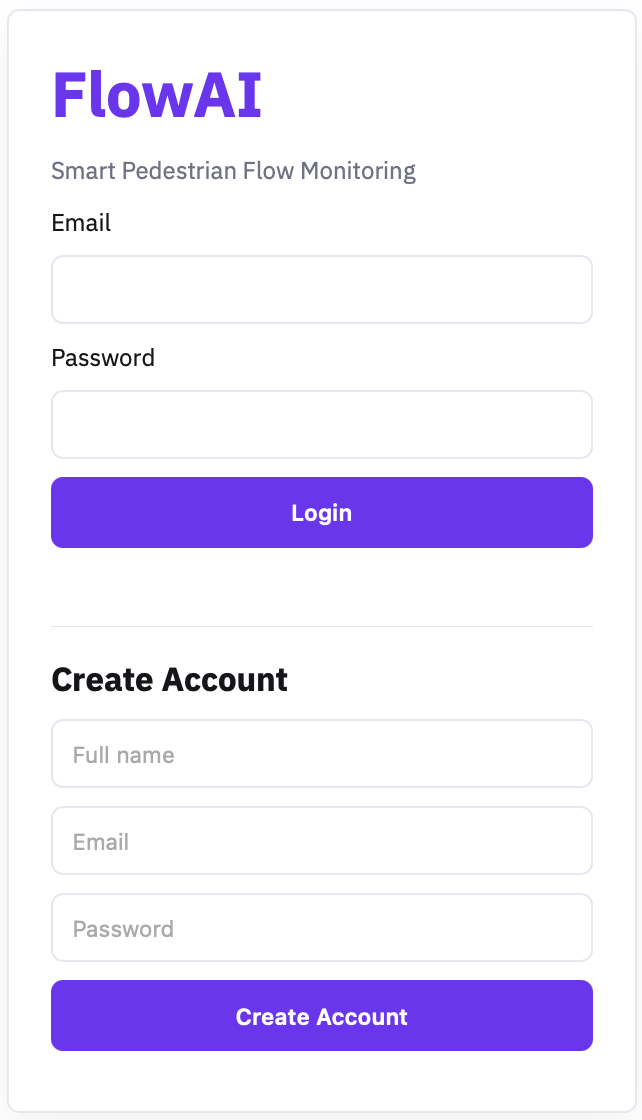
\includegraphics[width=0.5\textwidth]{figures/screenshot-login.png}
    \caption{Login and account creation interface}
    \label{fig:ui-login}
\end{figure}

\begin{figure}[H]
    \centering
    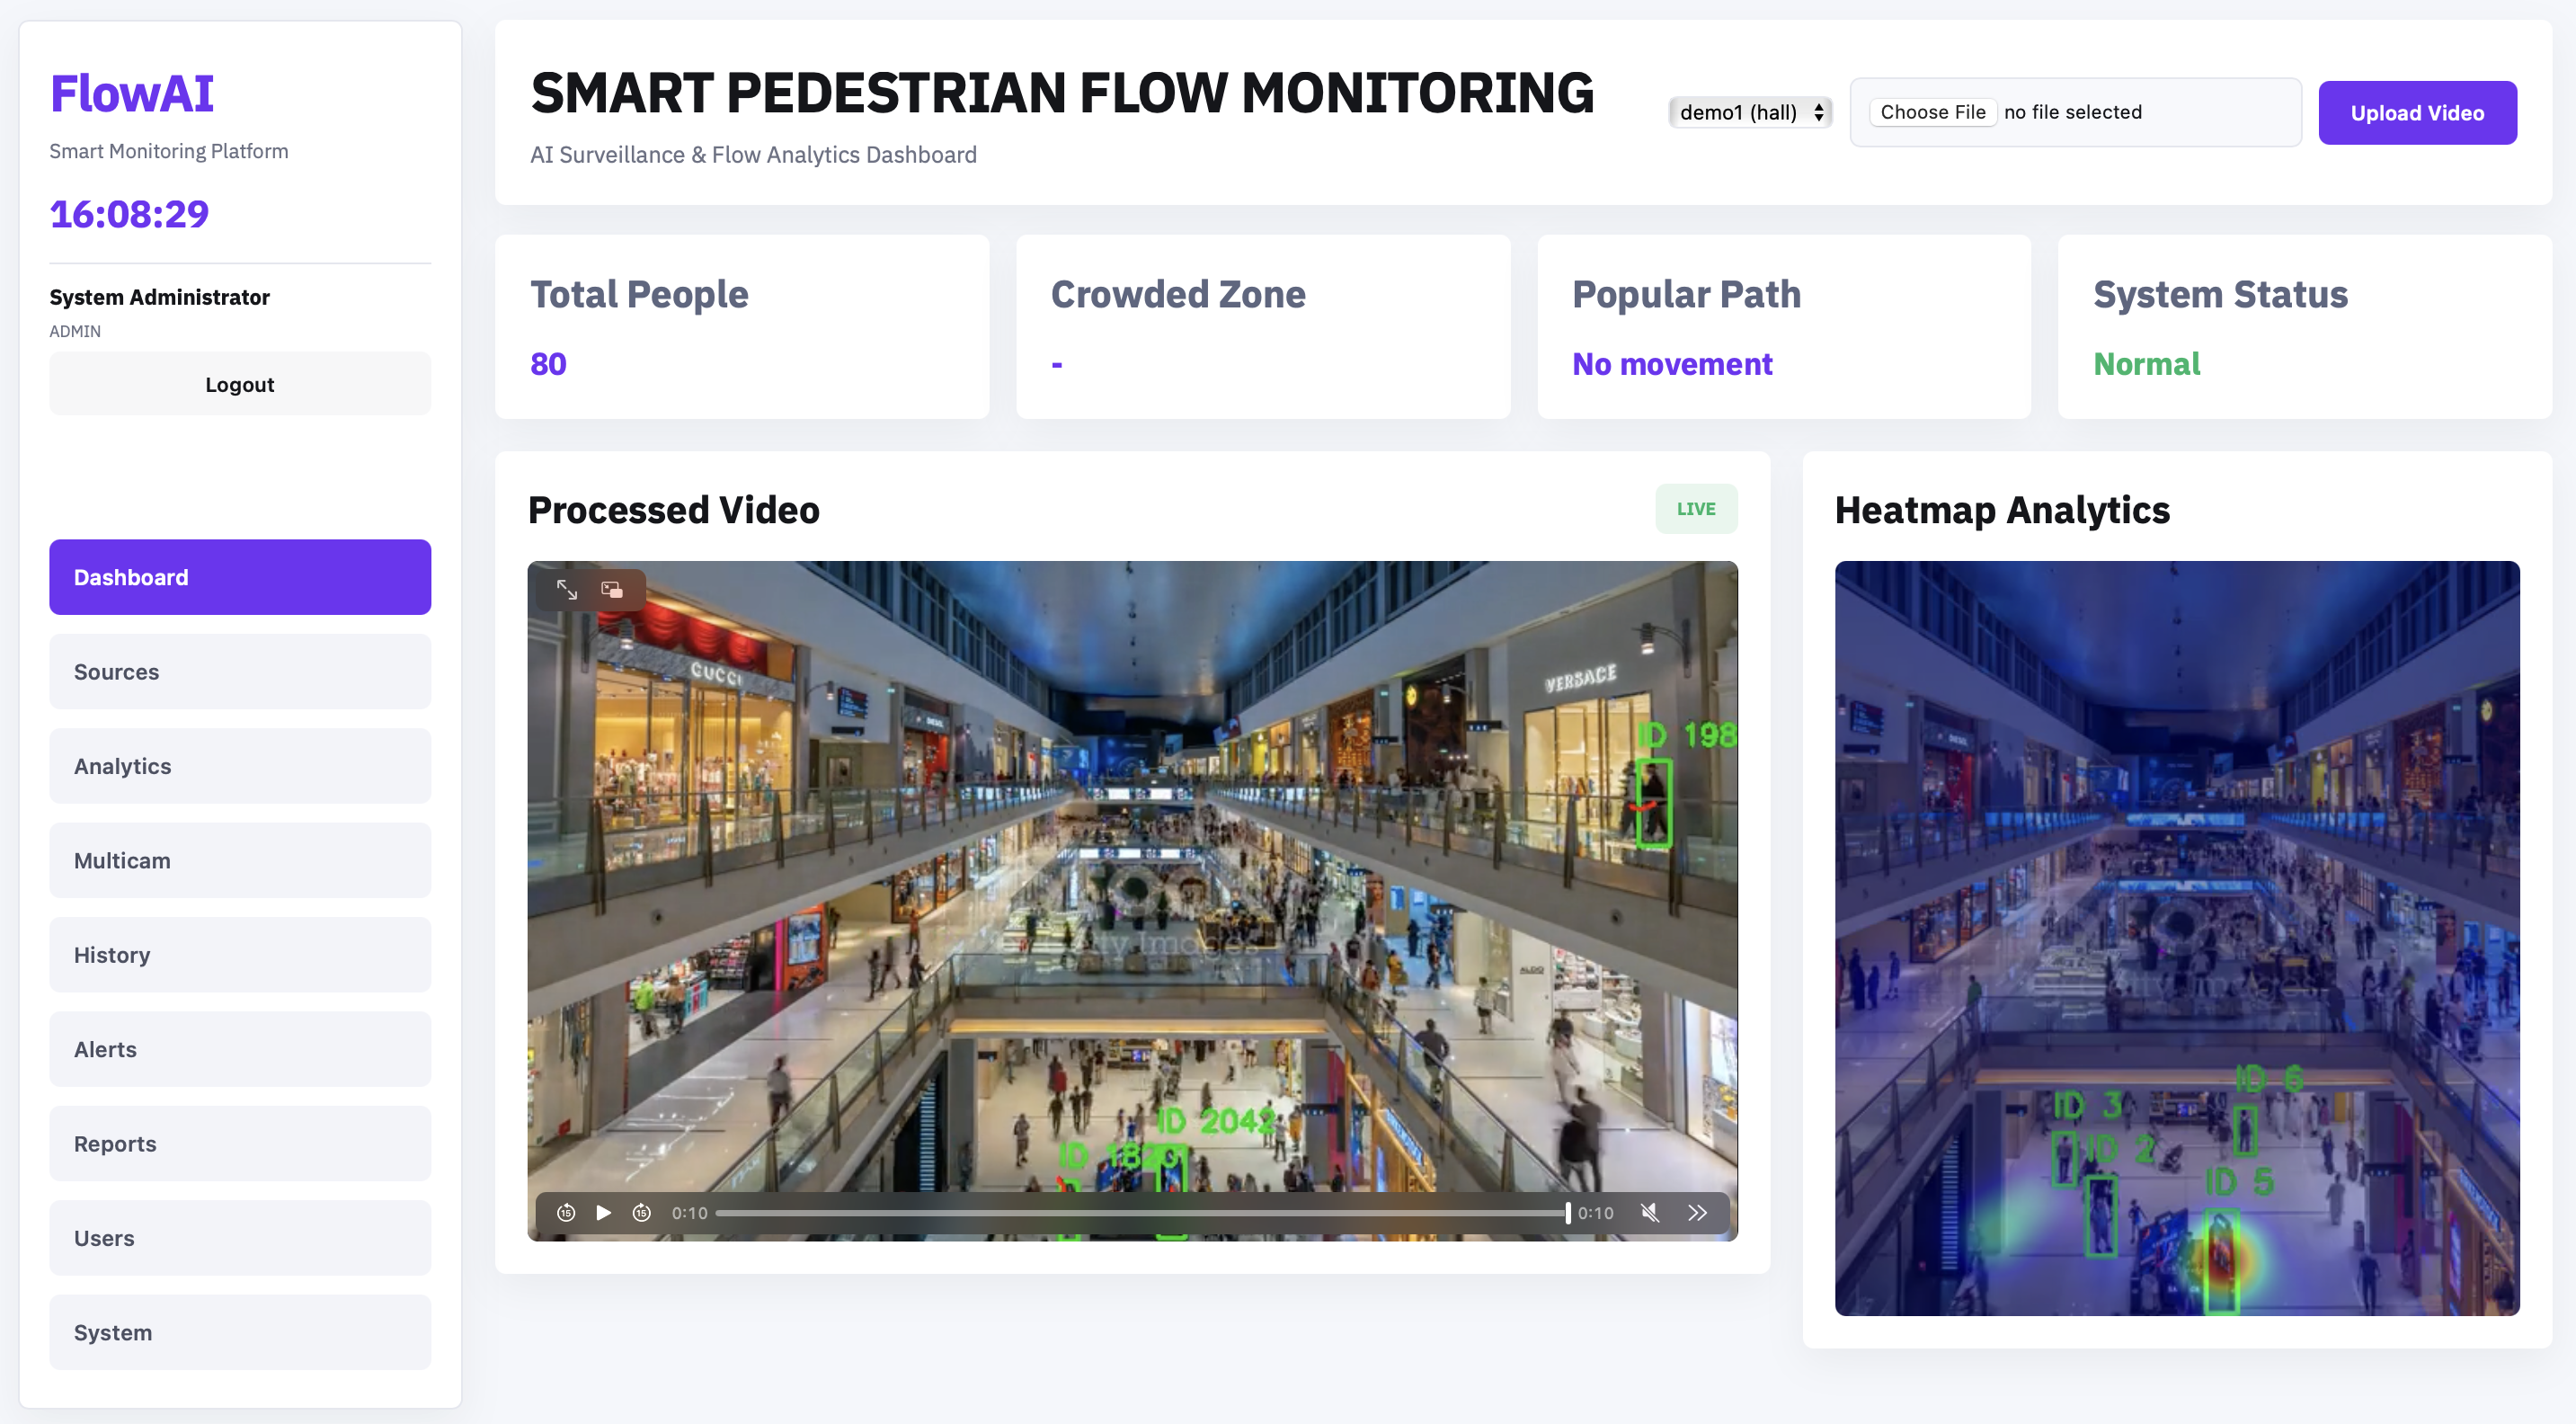
\includegraphics[width=0.95\textwidth]{figures/screenshot-dashboard.png}
    \caption{Main dashboard with processed video, KPIs, and heatmap analytics}
    \label{fig:ui-dashboard}
\end{figure}

\begin{figure}[H]
    \centering
    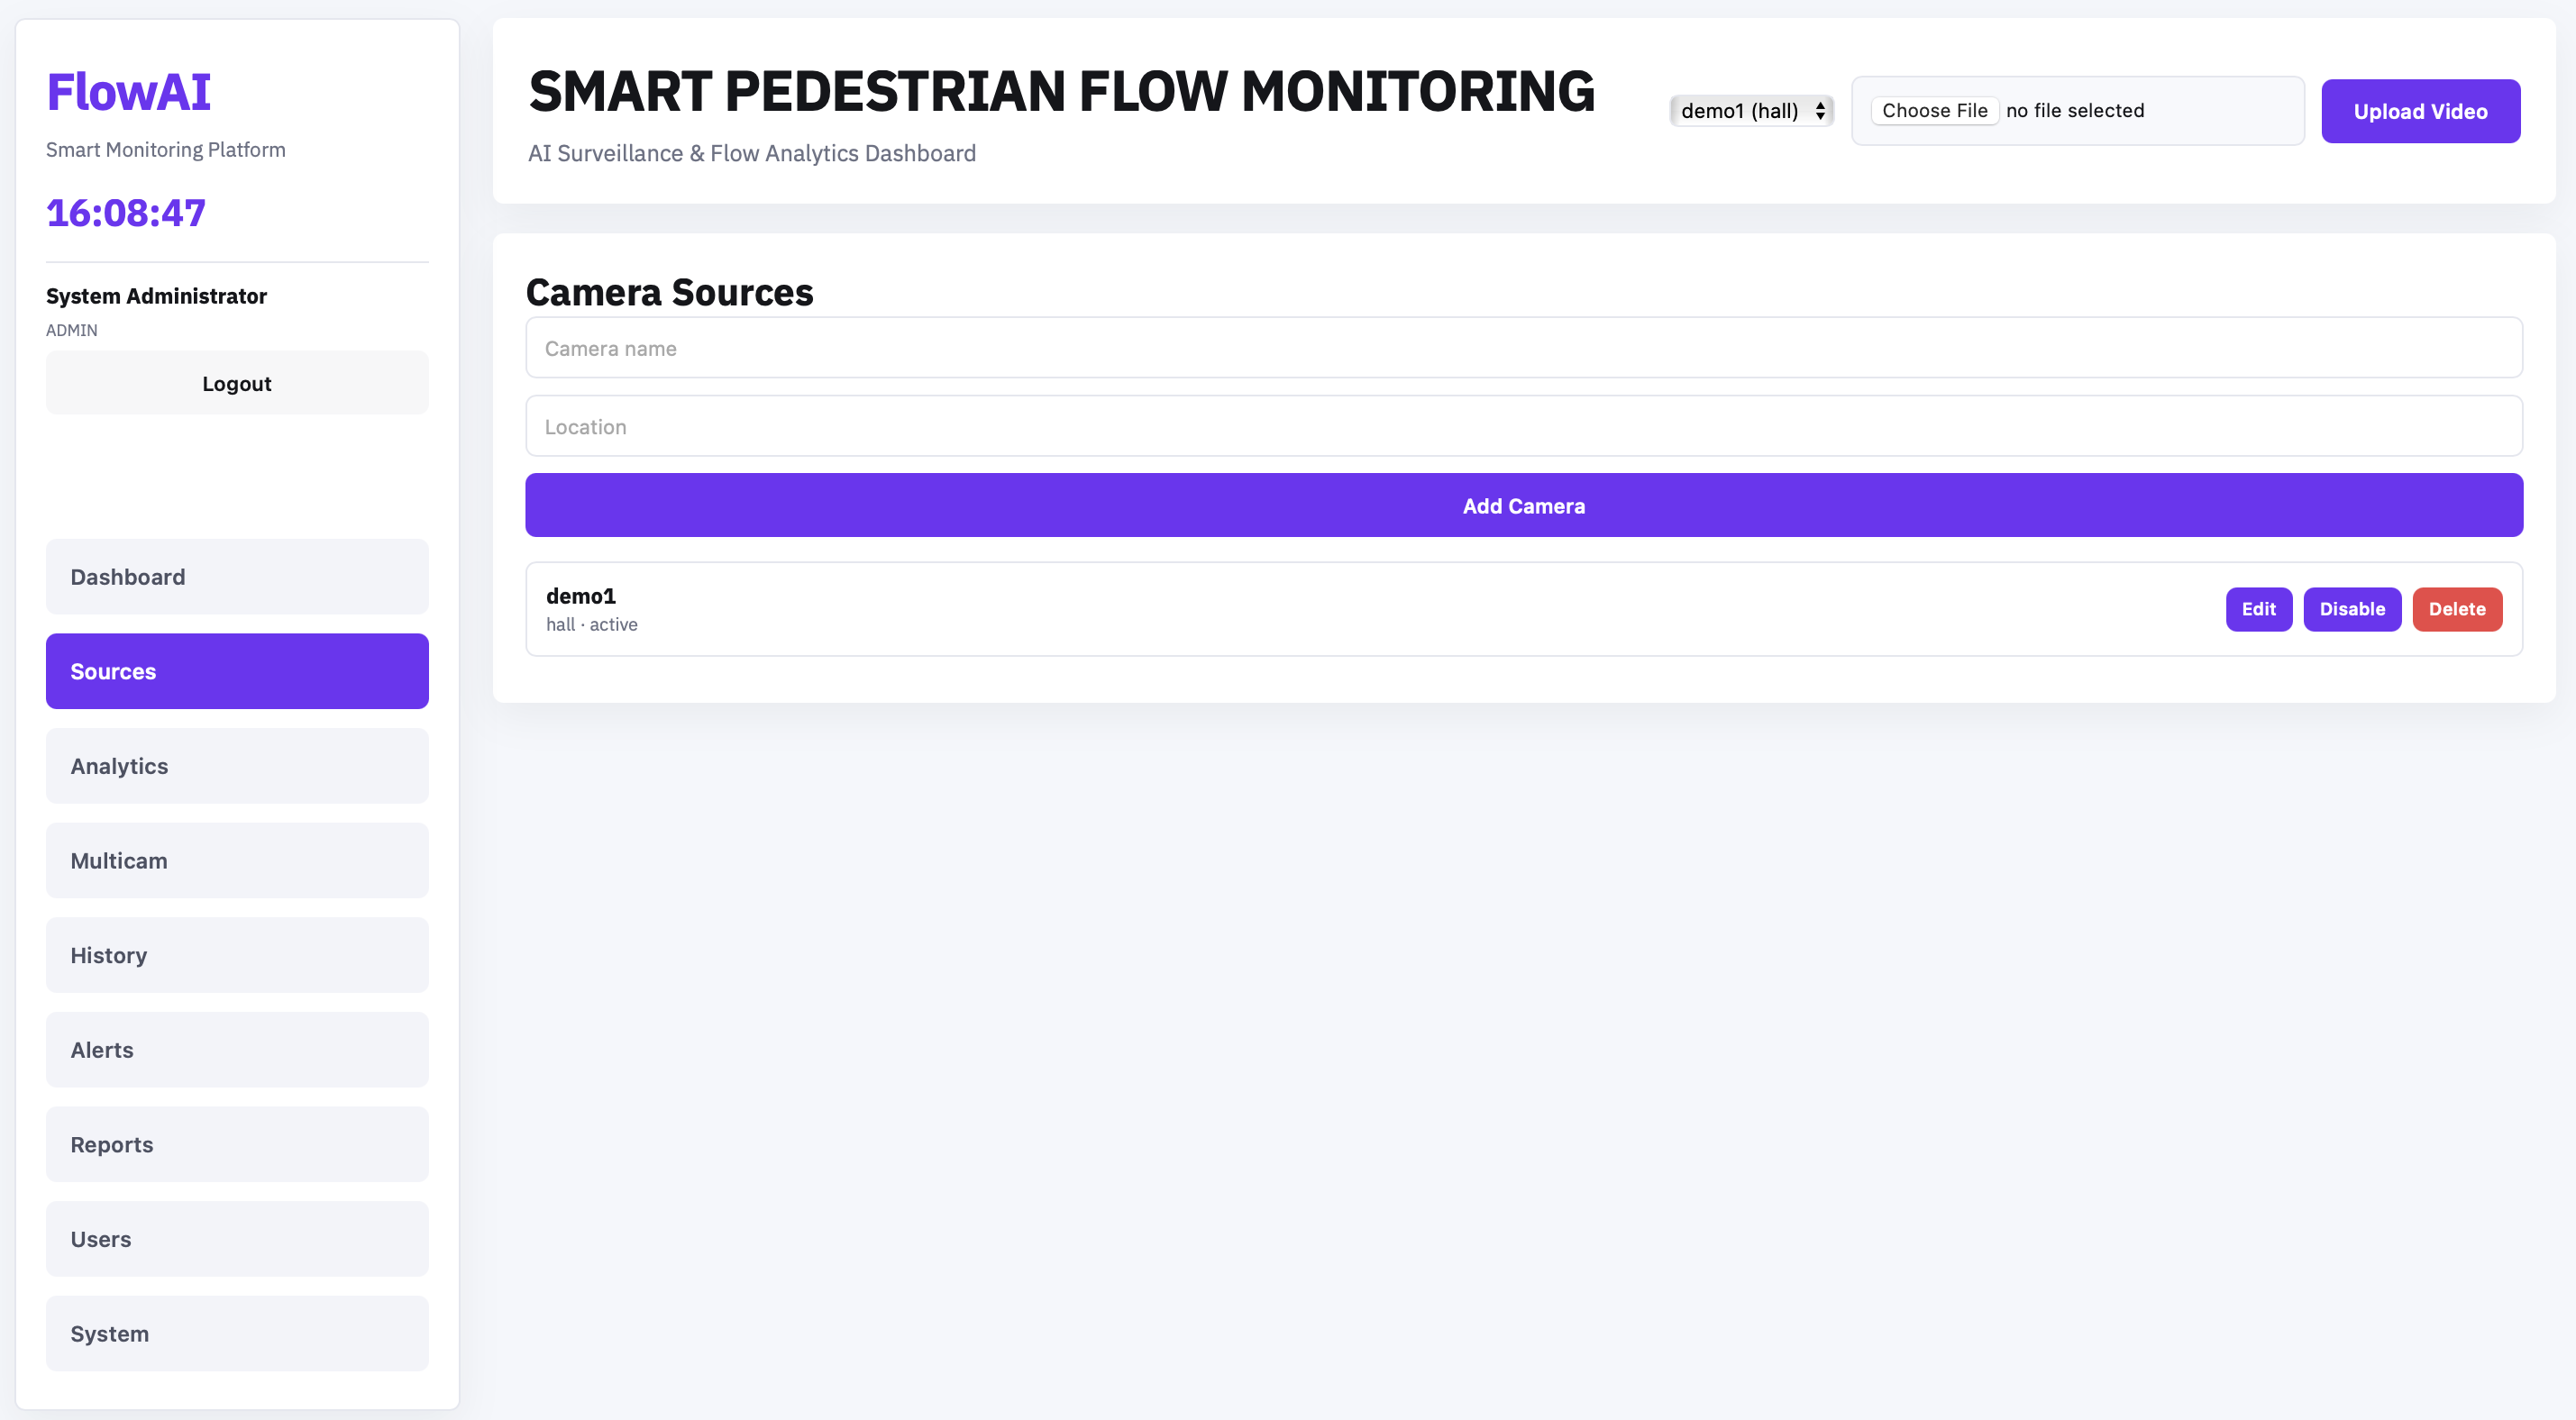
\includegraphics[width=0.95\textwidth]{figures/screenshot-camera-management.png}
    \caption{Camera source management interface}
    \label{fig:ui-camera-management}
\end{figure}

\begin{figure}[H]
    \centering
    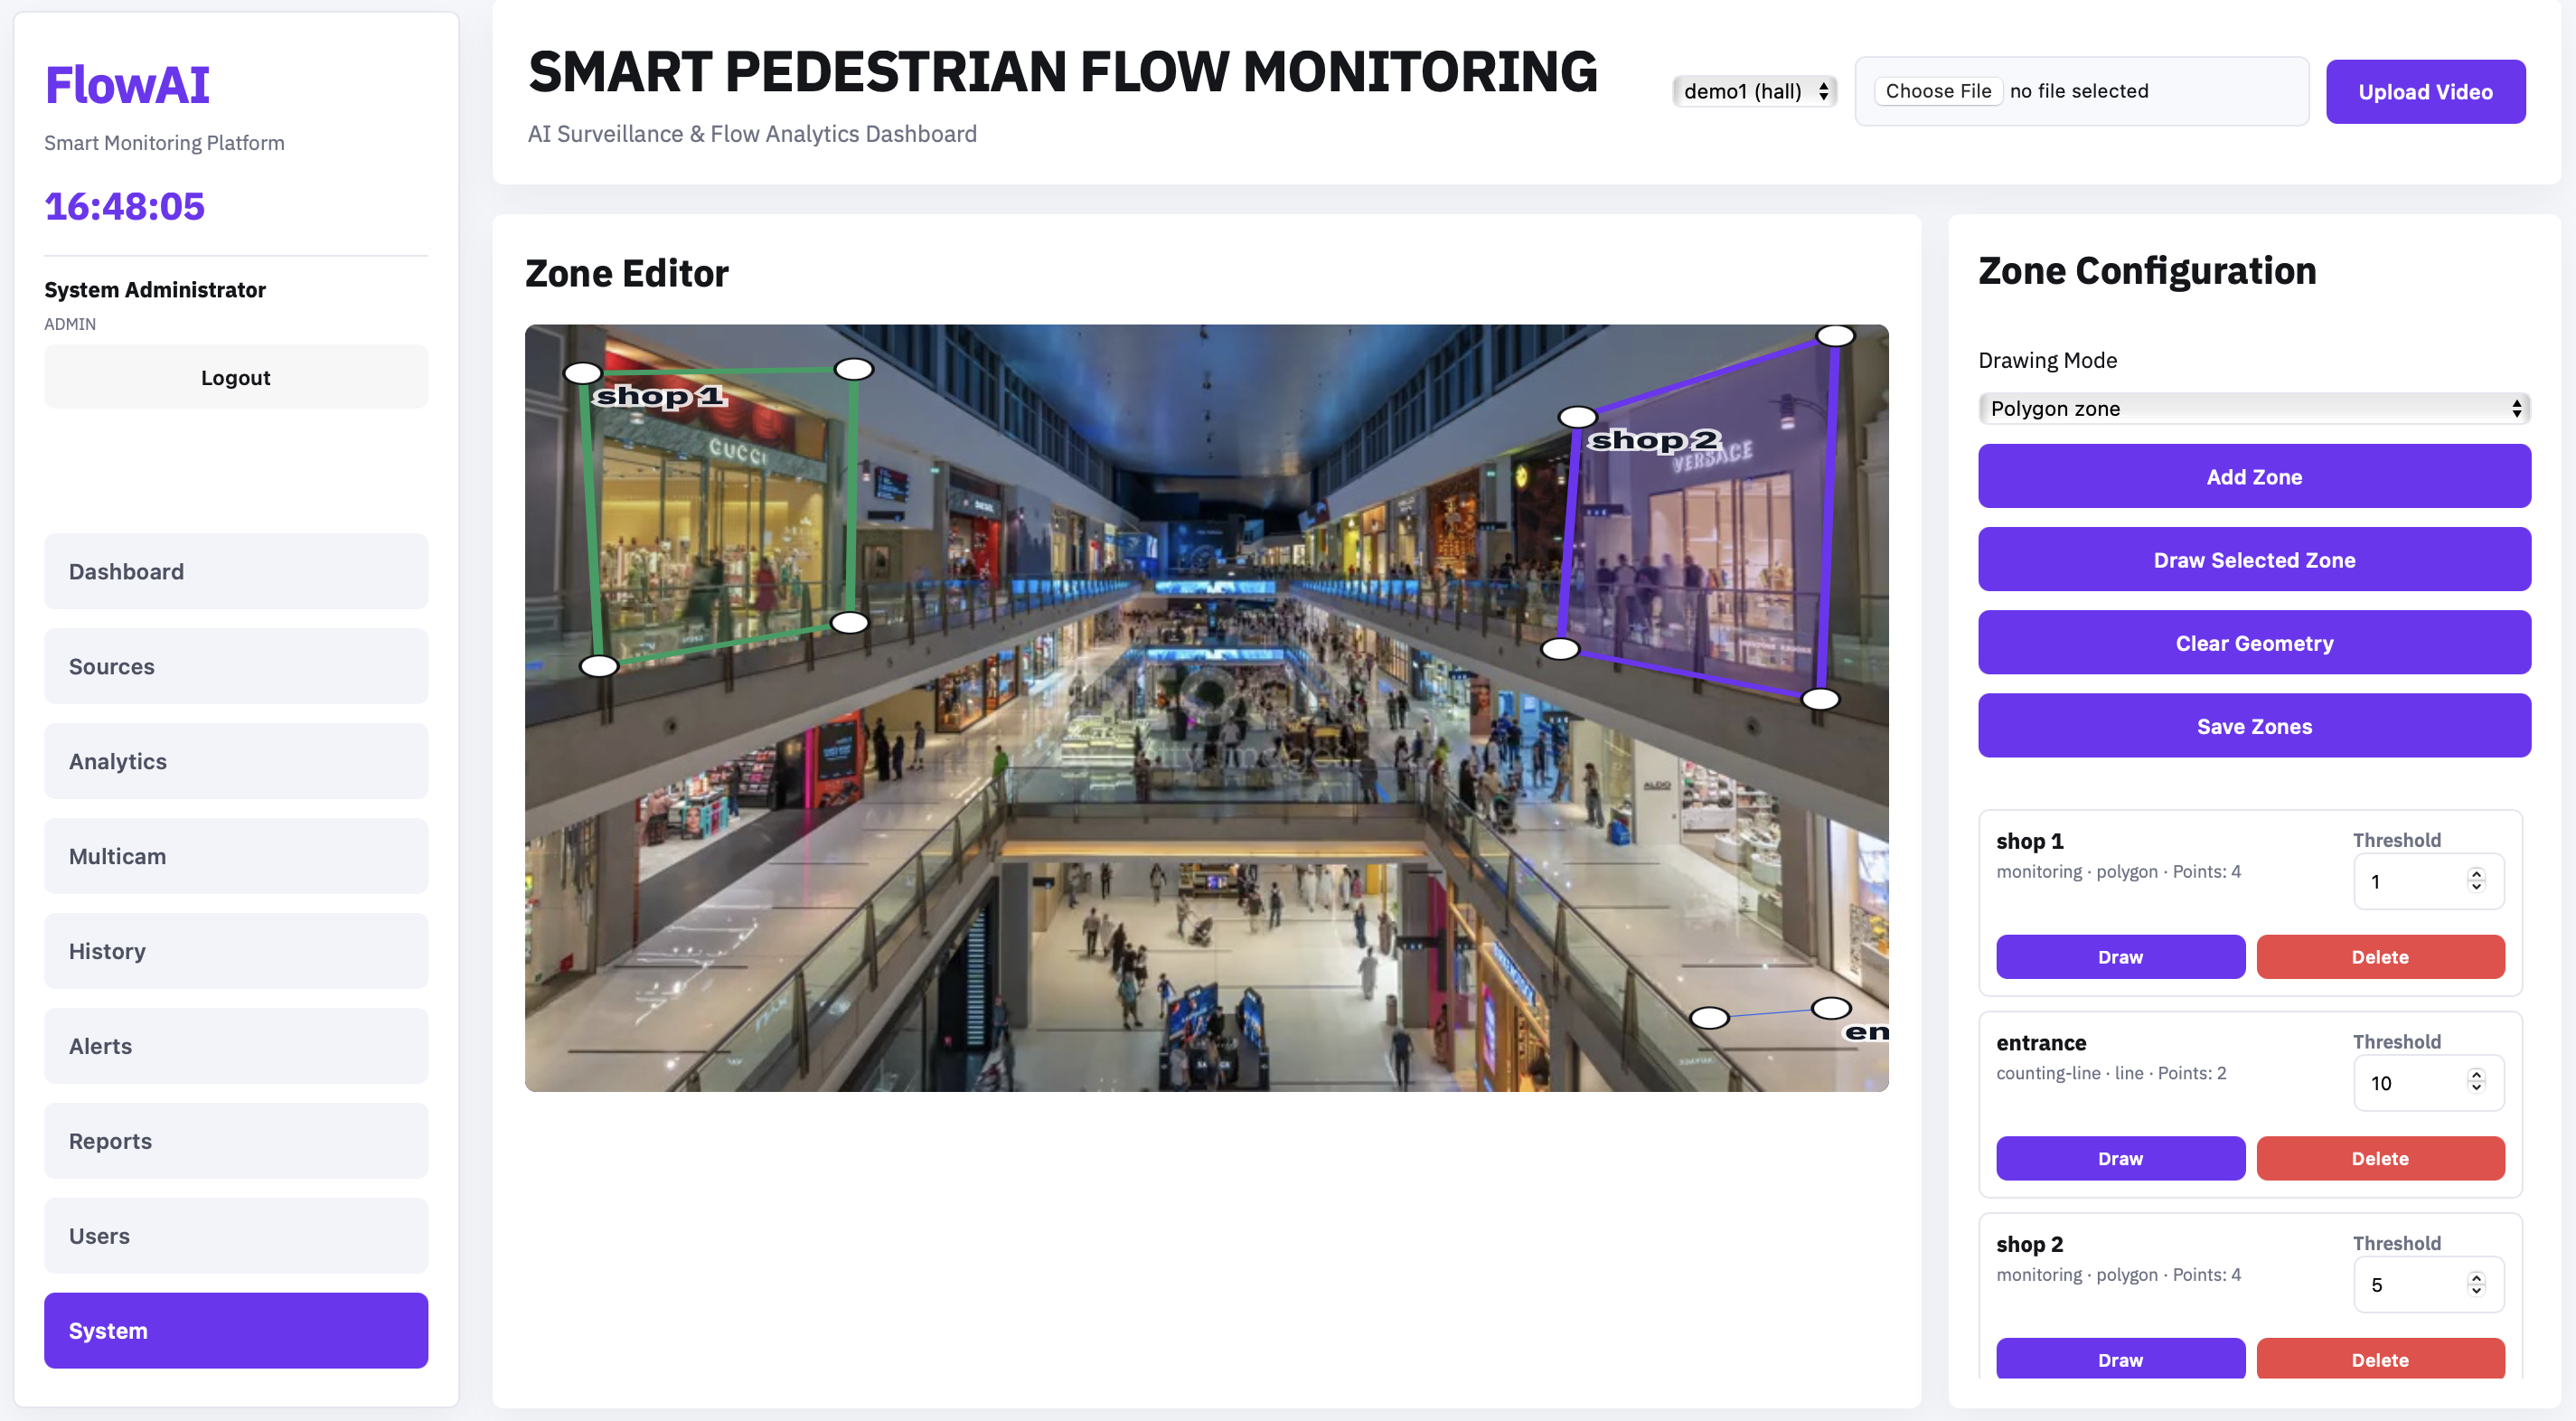
\includegraphics[width=0.95\textwidth]{figures/screenshot-zone-configuration.png}
    \caption{Zone configuration and threshold setting interface}
    \label{fig:ui-zone-config}
\end{figure}

\begin{figure}[H]
    \centering
    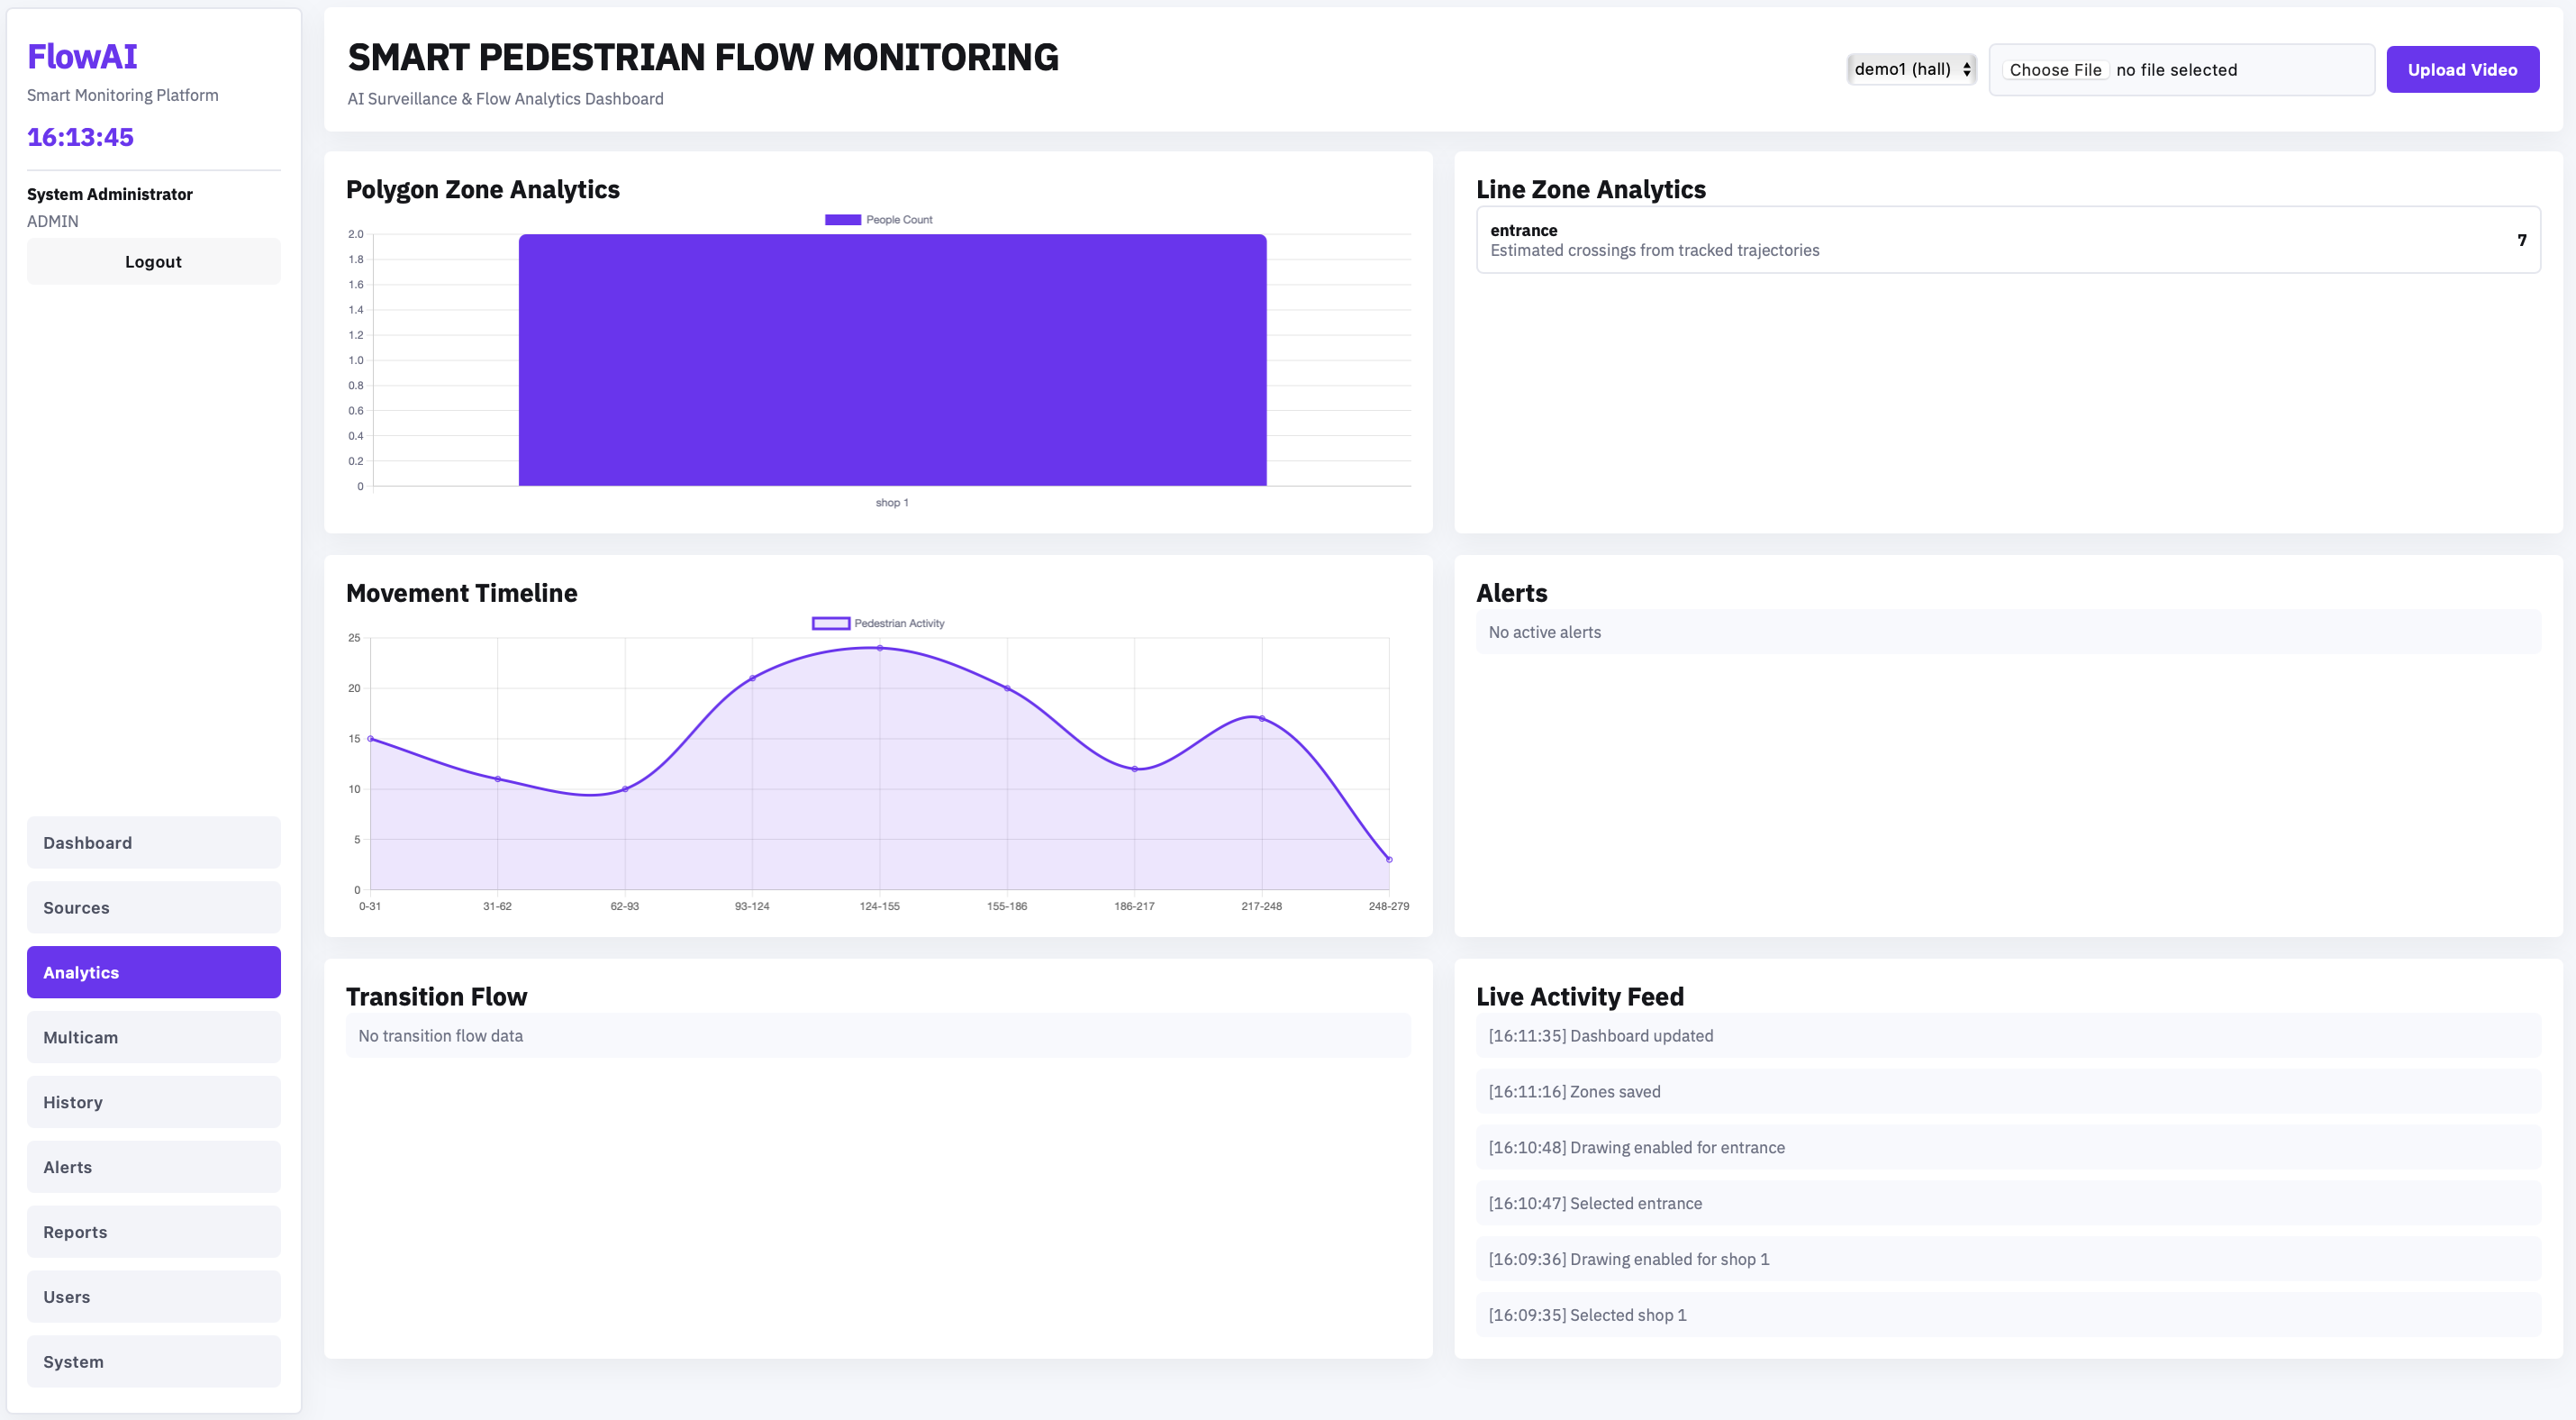
\includegraphics[width=0.95\textwidth]{figures/screenshot-analytics.png}
    \caption{Analytics page with zone counts, movement timeline, alerts, and transition flow}
    \label{fig:ui-analytics}
\end{figure}

\begin{figure}[H]
    \centering
    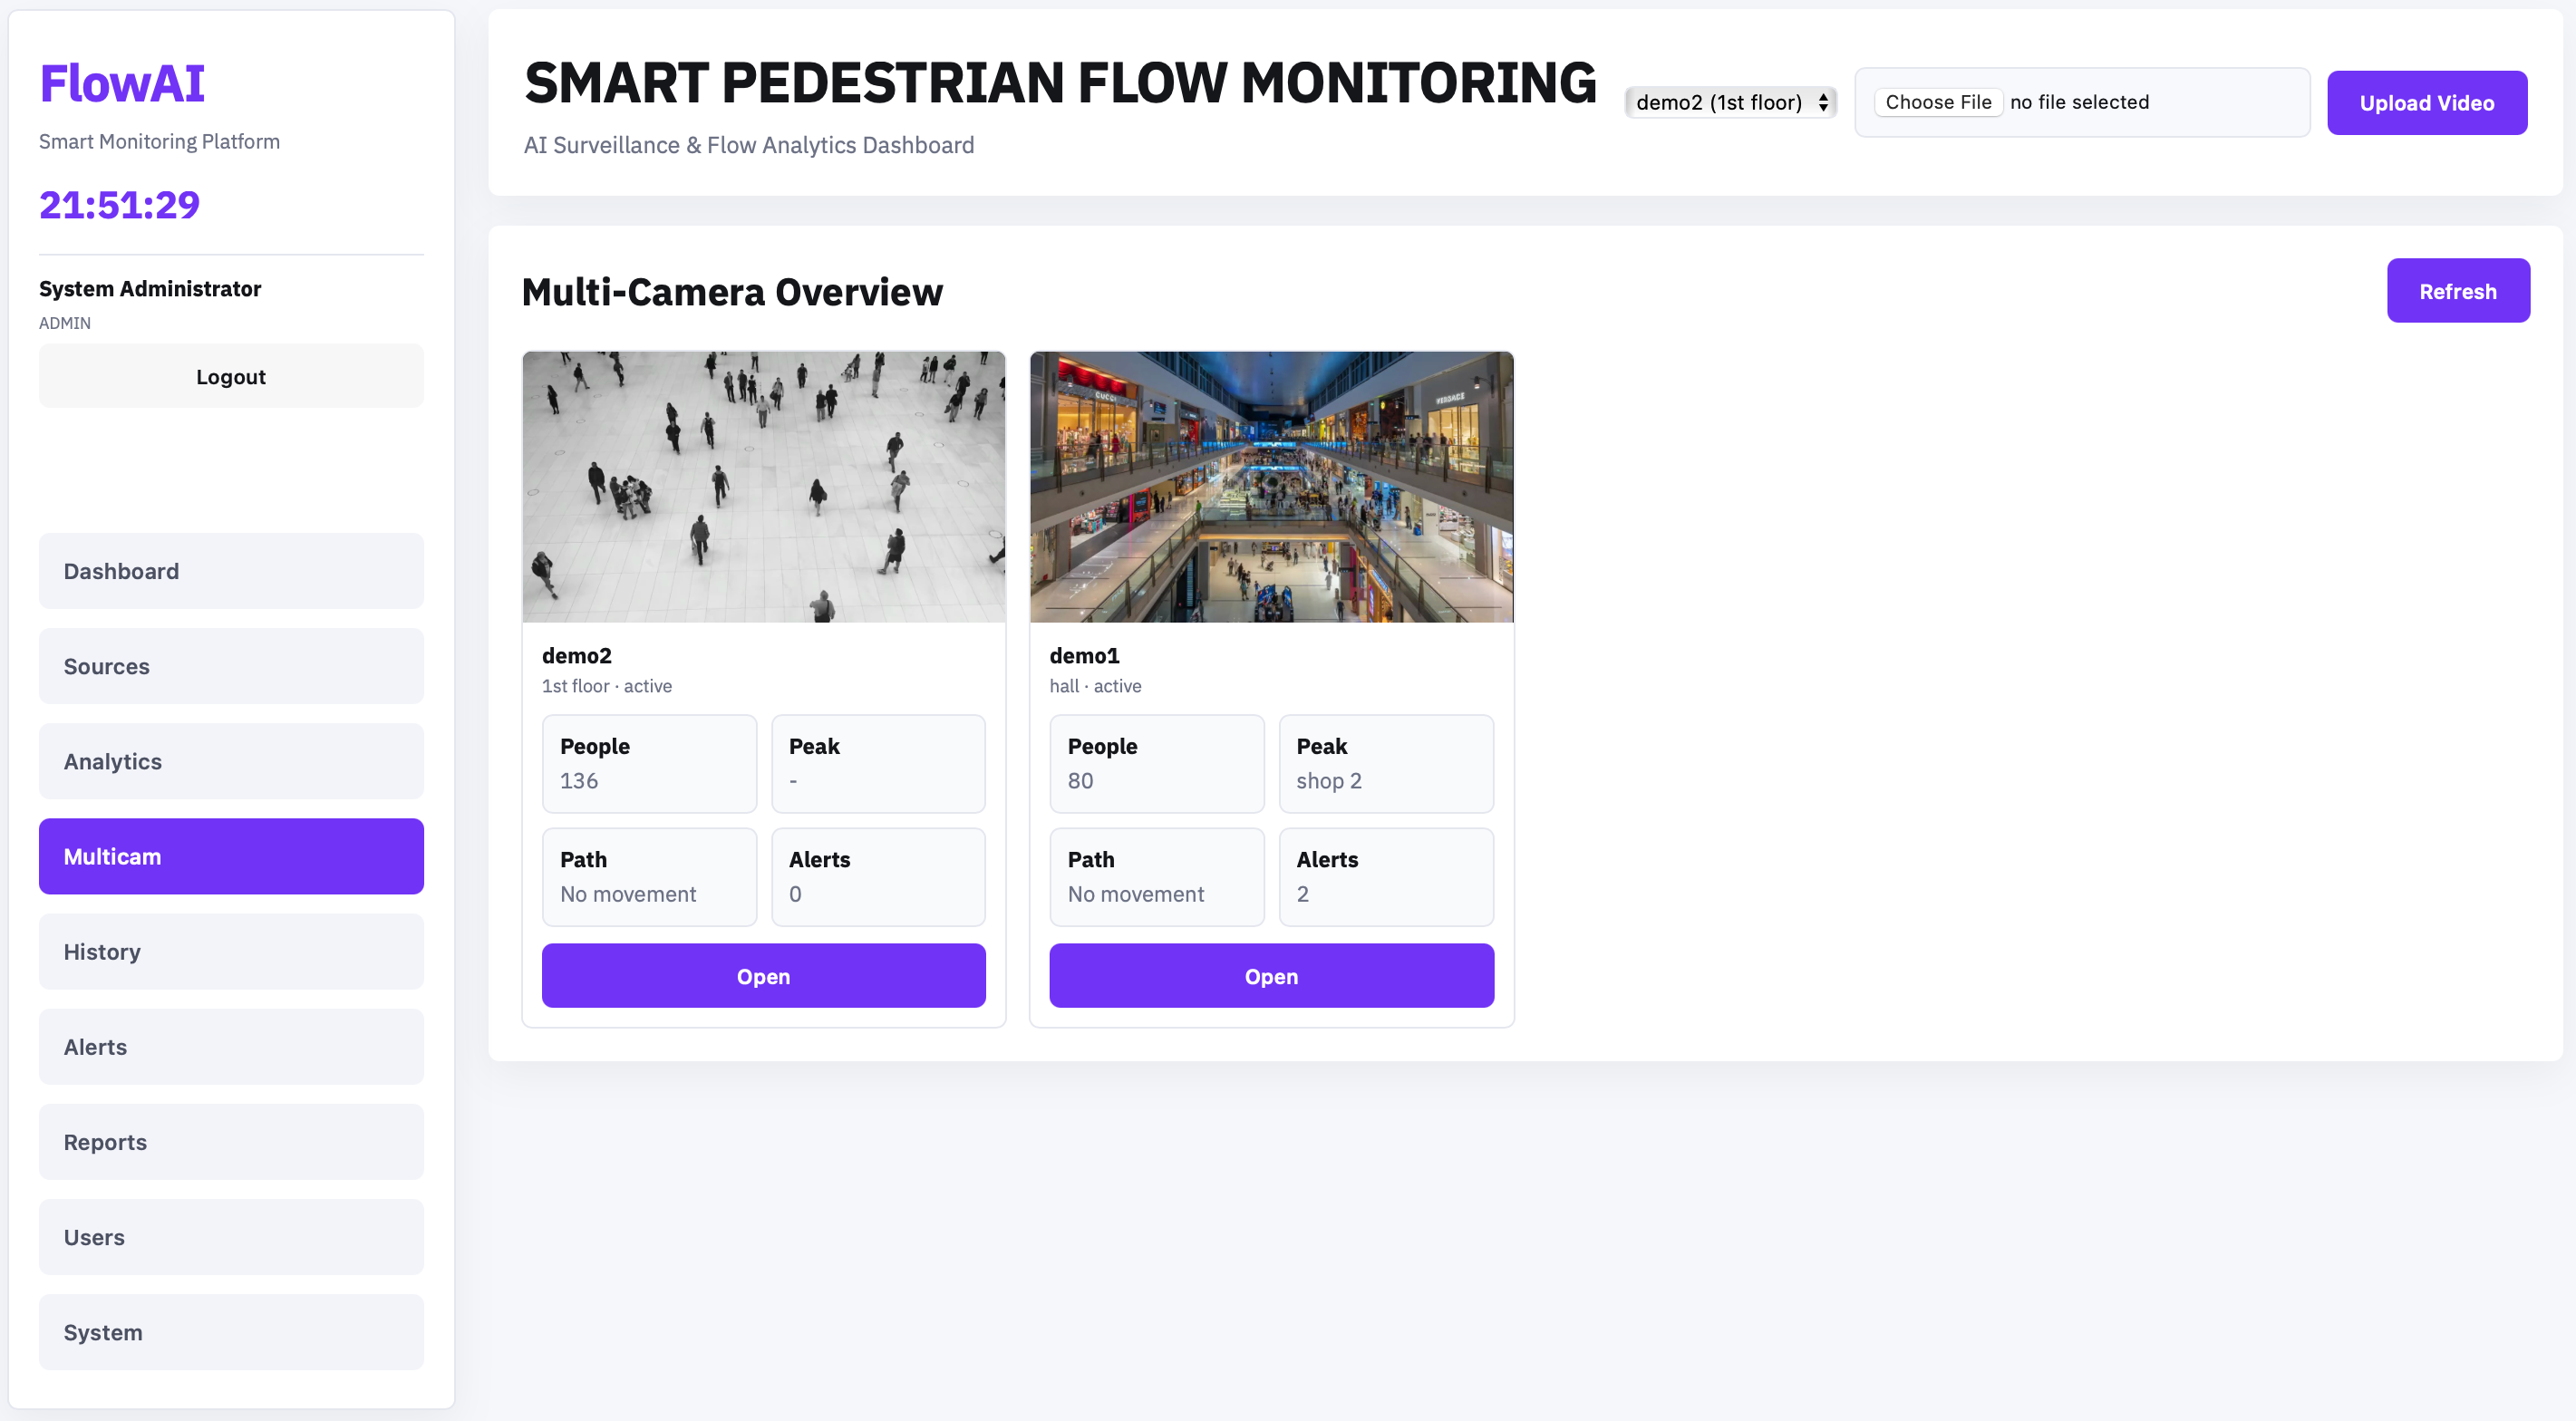
\includegraphics[width=0.95\textwidth]{figures/screenshot-multicam.png}
    \caption{Overview of multi-camera system}
    \label{fig:ui-analytics}
\end{figure}

\begin{figure}[H]
    \centering
    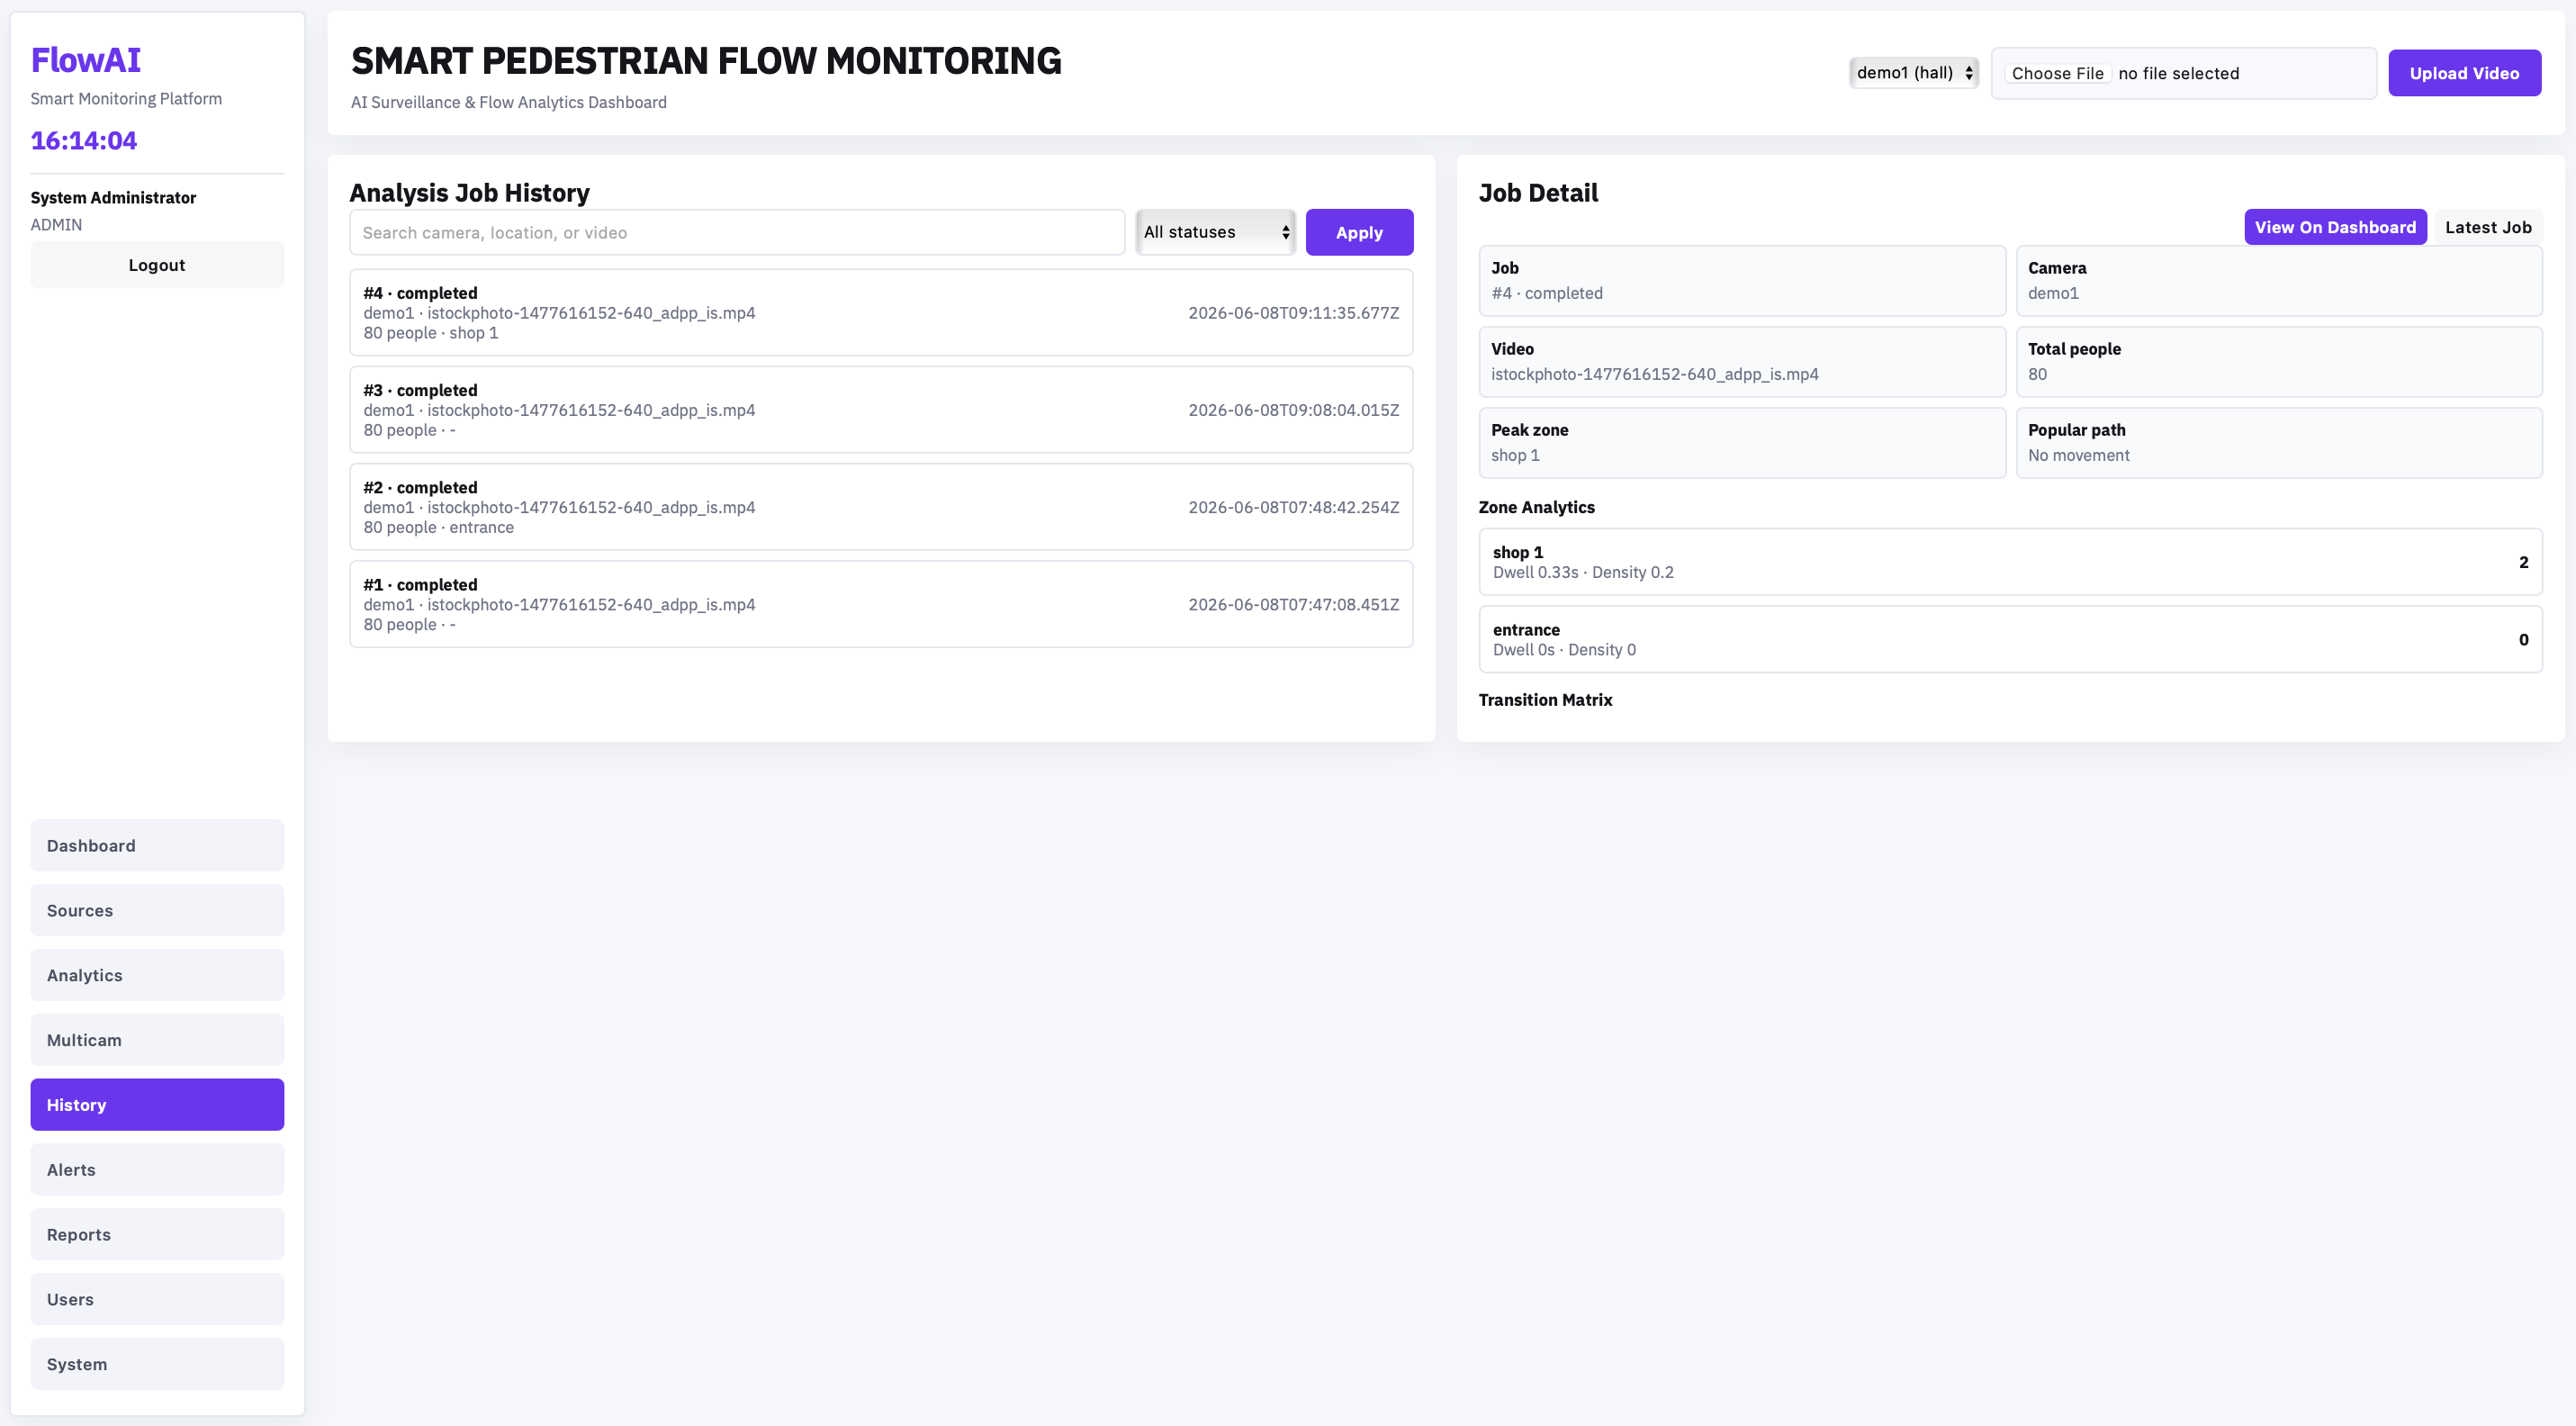
\includegraphics[width=0.95\textwidth]{figures/screenshot-history.png}
    \caption{Analysis job history and job detail interface}
    \label{fig:ui-history}
\end{figure}

\begin{figure}[H]
    \centering
    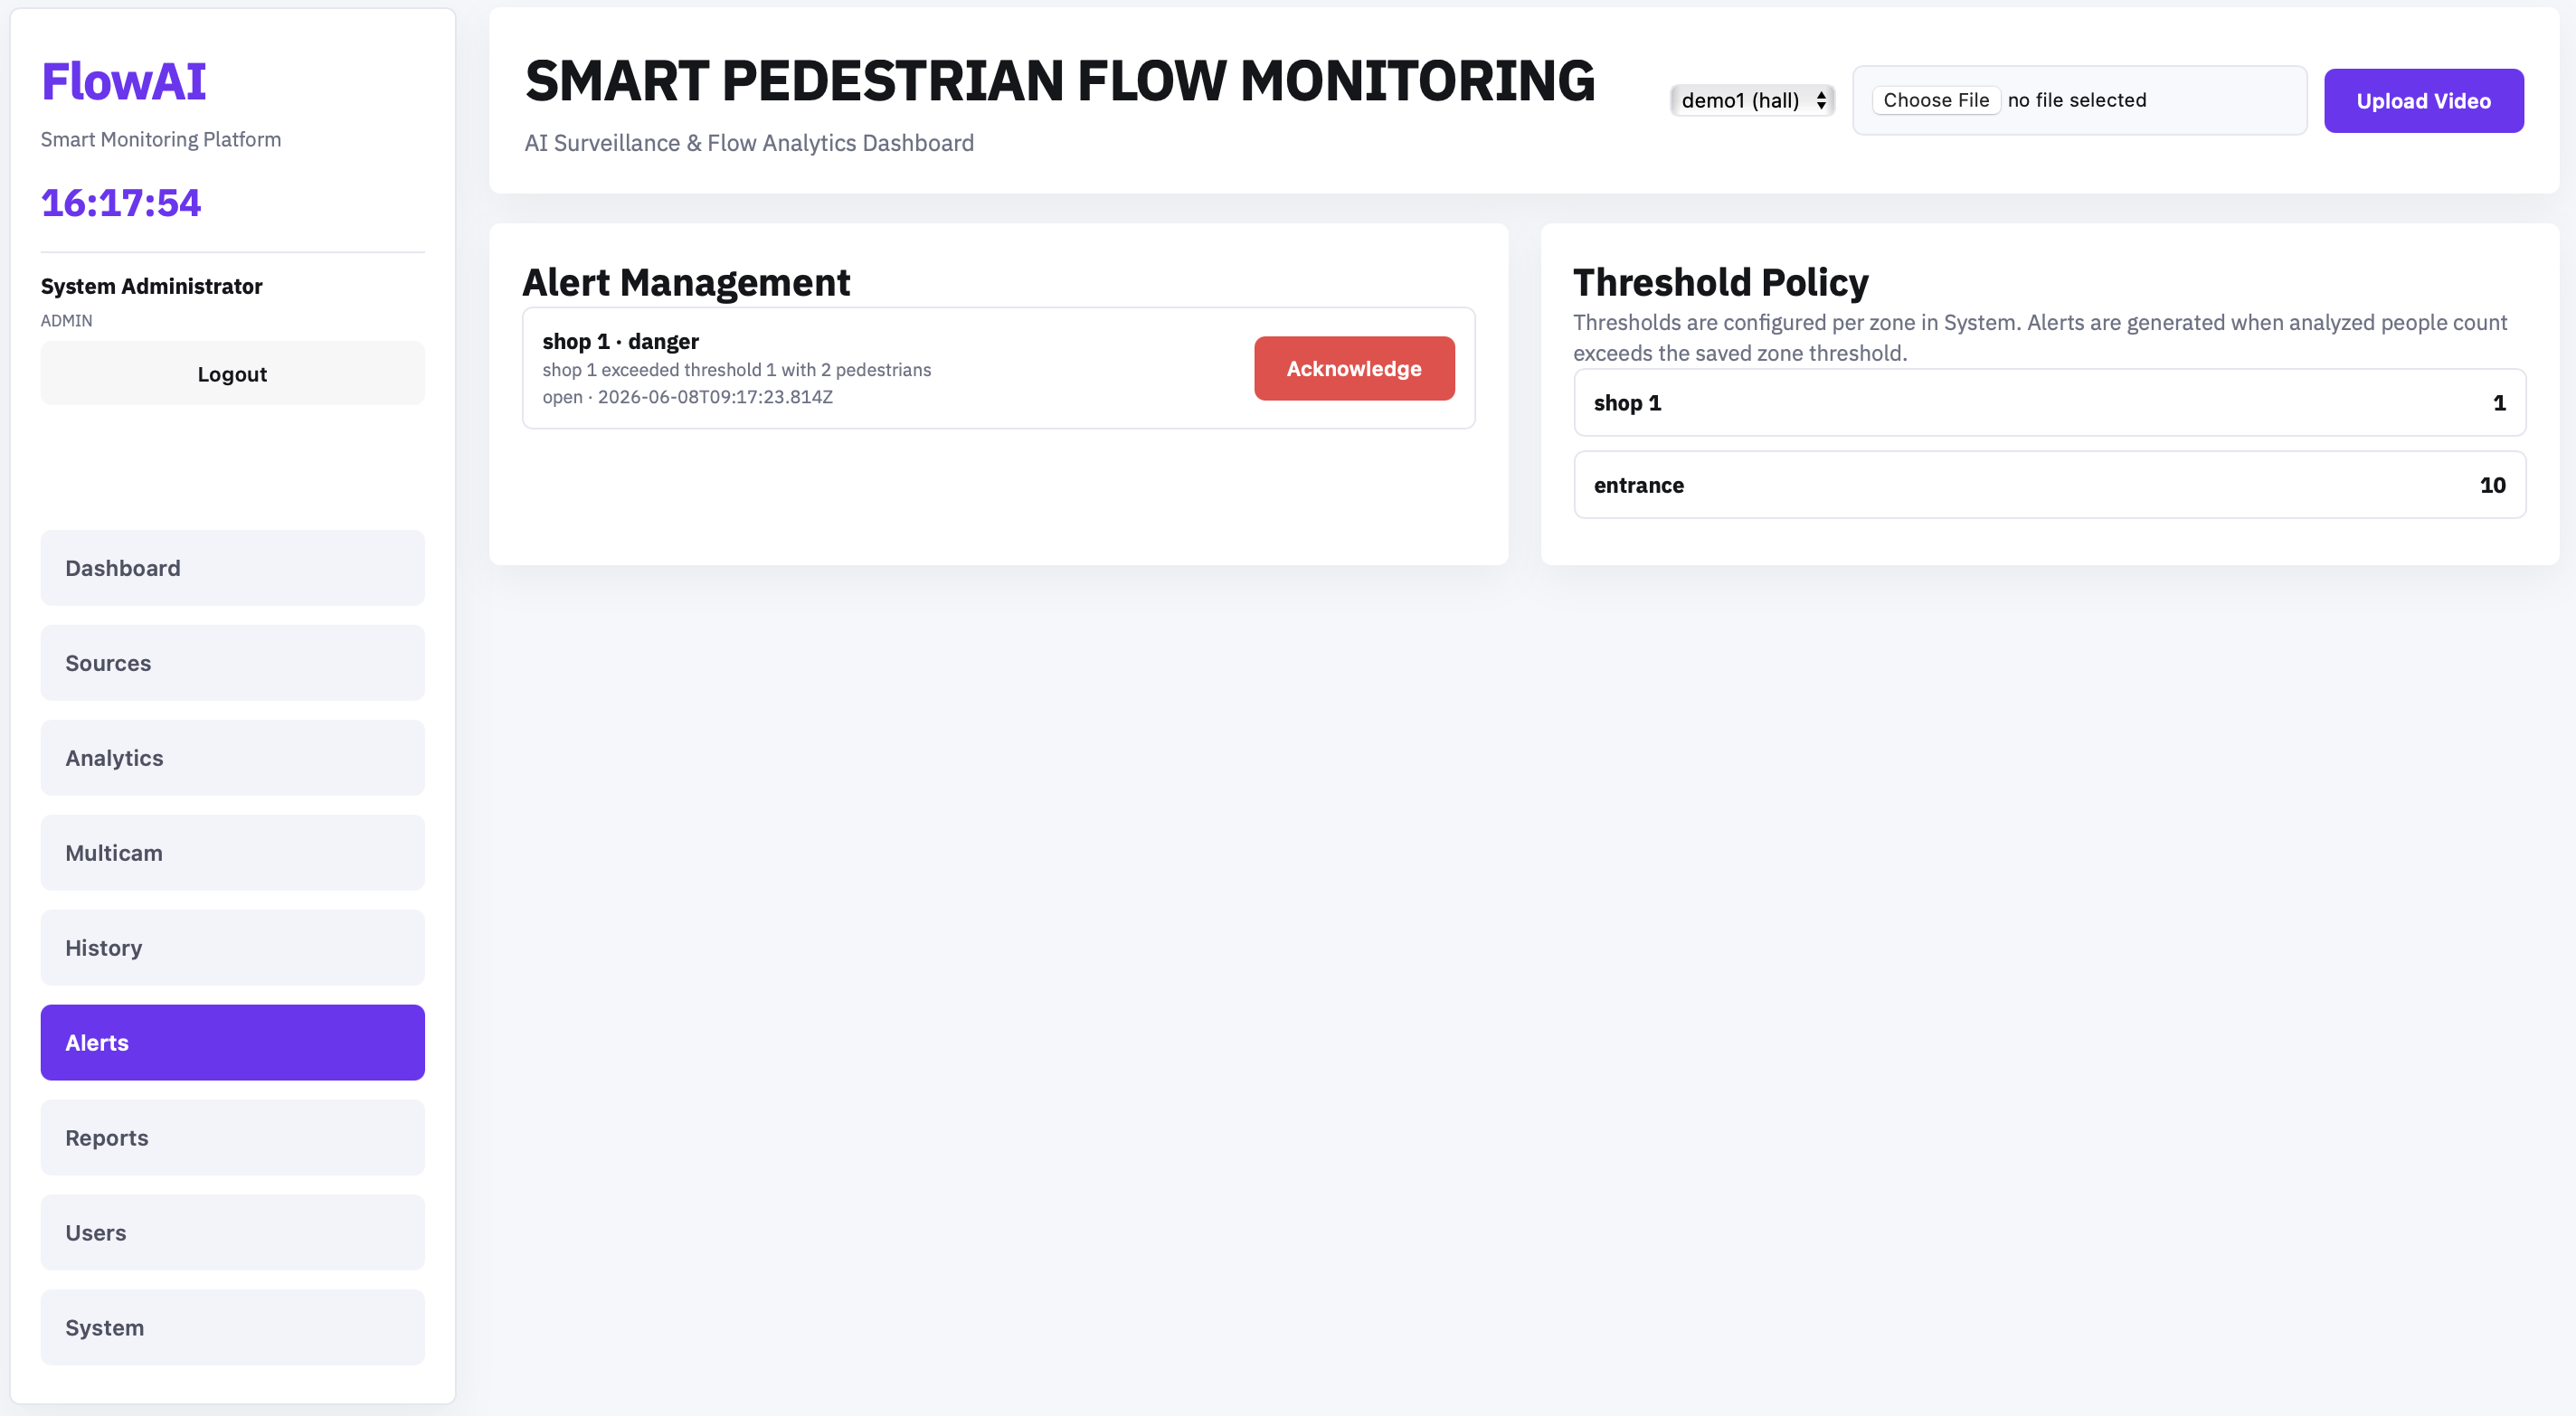
\includegraphics[width=0.95\textwidth]{figures/screenshot-alert.png}
    \caption{Alert management and threshold policy interface}
    \label{fig:ui-alert}
\end{figure}

\begin{figure}[H]
    \centering
    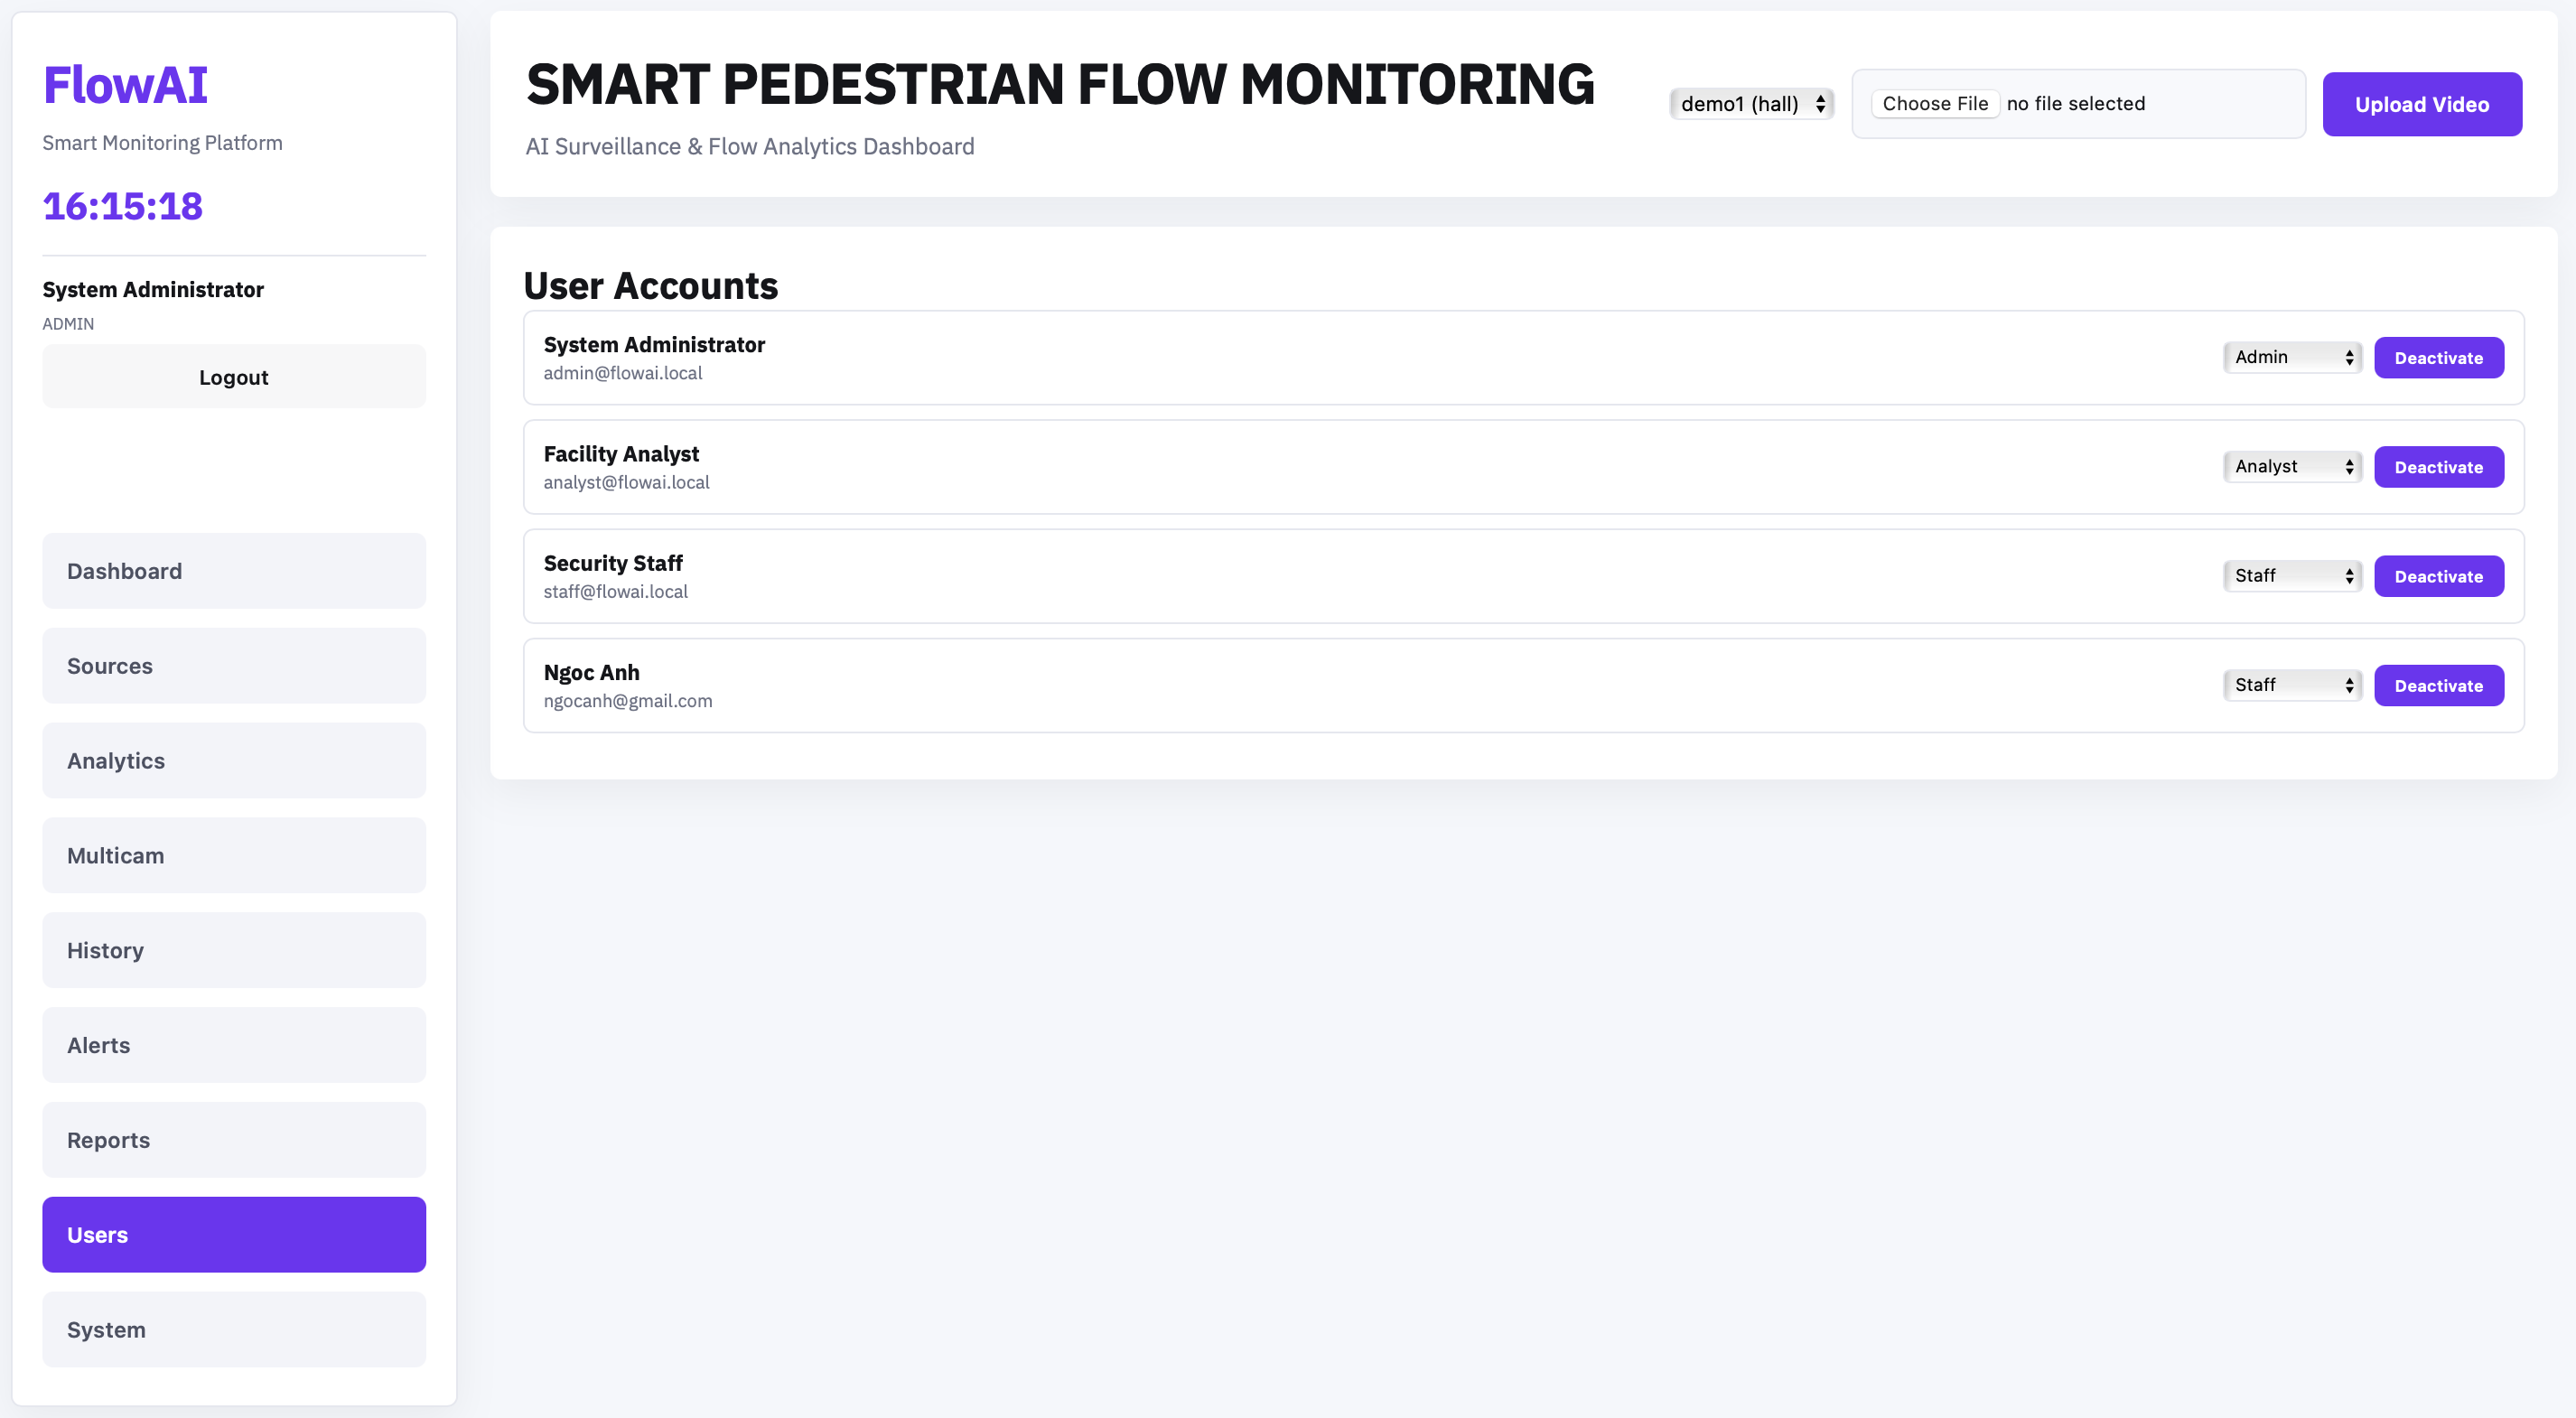
\includegraphics[width=0.95\textwidth]{figures/screenshot-user-management.png}
    \caption{User account management interface}
    \label{fig:ui-user-management}
\end{figure}

\begin{figure}[H]
    \centering
    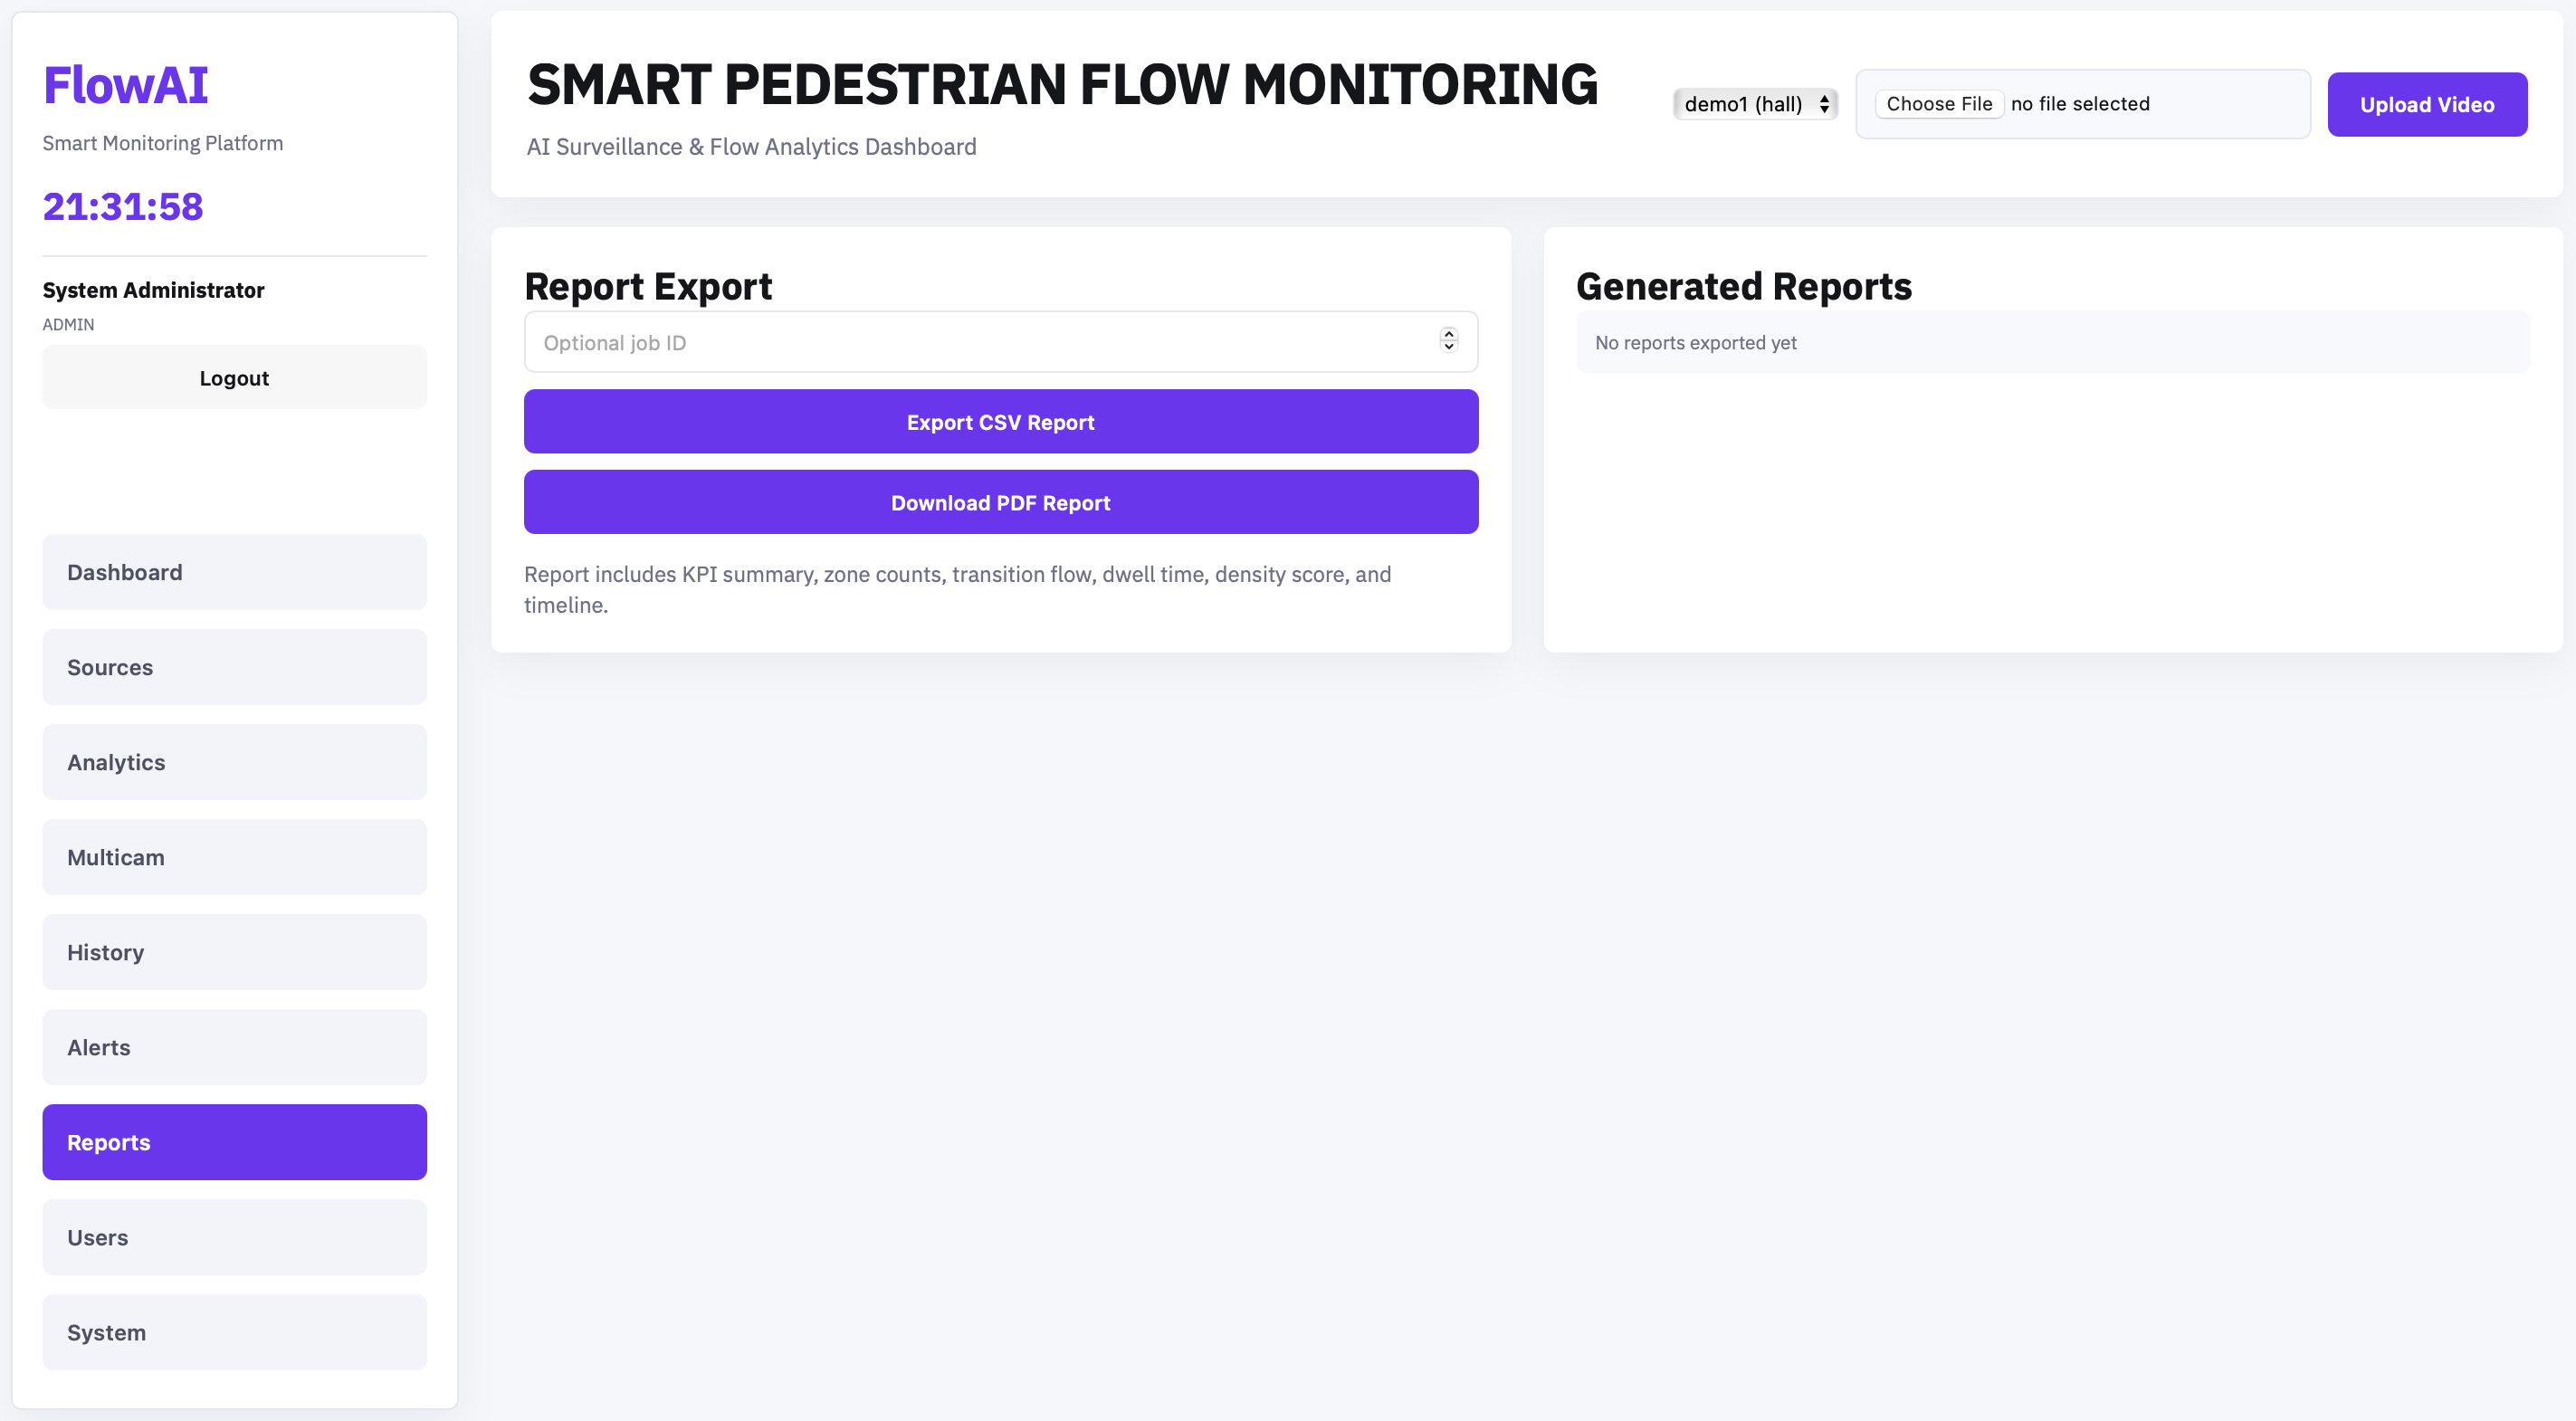
\includegraphics[width=0.95\textwidth]{figures/Screenshot-reports.png}
    \caption{Report export and generated report history interface}
    \label{fig:ui-report}
\end{figure}

% =====================================================
% CHAPTER 6
% =====================================================
\chapter{SYSTEM TESTING}

\section{Testing Purpose and Strategy}

The purpose of system testing is not to prove that the prototype has no defects. Instead, testing is used to evaluate whether the implemented system behaves correctly under normal cases, invalid cases, boundary cases, integration cases, and acceptance-level scenarios.

The test suite is designed based on the main use cases and actual implemented modules of the Smart Pedestrian Flow Monitoring and Analytics System. The tested scope includes authentication, role-based access control, camera source management, video upload, zone configuration, pedestrian analysis, dashboard visualization, alert management, and report export.

Testing contribution: Vu Thuy Linh was responsible for API/UI testing, smoke testing, end-to-end flow validation, bug reporting, and fix verification. The results below focus on validating the implemented prototype under local demo conditions rather than claiming full production readiness.

Testing environment: Localhost with Node.js, Python 3, PostgreSQL, and a modern web browser.

\section{Test Status Definitions}

Only three statuses are used in this chapter:

\begin{longtable}{|p{3.4cm}|p{10.2cm}|}
\hline
\rowcolor{HeaderBlue}
\textbf{Status} & \textbf{Meaning} \\
\hline
Passed & The actual result matches the expected result in the confirmed local demo environment. \\
\hline
Failed & The actual result does not match the expected result, or the tested feature is not supported in the current prototype. \\
\hline
Pending & The test case is valid, but it was not fully executed because the team did not have enough data, time, or environment setup. \\
\hline
\end{longtable}

\section{API Smoke Test Execution}

The automated API smoke test was executed with the following command:

\begin{lstlisting}[language=bash]
BASE_URL=http://127.0.0.1:3000 npm run test:api
\end{lstlisting}

The executed smoke test contains 11 core API checks. The result was:

\begin{lstlisting}
PASS TC-01 invalid login is rejected
PASS TC-02 admin login succeeds
PASS TC-03 camera list is available
PASS TC-04 smoke camera can be created
PASS TC-05 zones can be saved and loaded
PASS TC-06 multicamera overview is available
PASS TC-07 completed job can be discovered
PASS TC-08 latest stats expose analytics
PASS TC-09 job detail exposes analytics
PASS TC-10 CSV report export works
PASS TC-11 PDF report endpoint works
\end{lstlisting}

The smoke test validates the main backend flow quickly. It does not replace all manual UI testing or all edge-case testing.

\section{Test Case Summary}

\begin{longtable}{|p{2.5cm}|p{5.1cm}|p{2.3cm}|p{2.8cm}|p{1.9cm}|}
\hline
\rowcolor{HeaderBlue}
\textbf{Test ID} & \textbf{Test case} & \textbf{Related UC} & \textbf{Type} & \textbf{Status} \\
\hline
TC-AUTH-01 & Login with invalid password & UC-02 & Functional / Negative & Passed \\
\hline
TC-VIDEO-01 & Upload unsupported video file & UC-04 & Validation / Negative & Passed \\
\hline
TC-ANALYSIS-01 & Run analysis without configured zones & UC-04, UC-05 & Business rule / Boundary & Passed \\
\hline
TC-FLOW-01 & Detect zone-to-zone transition & UC-09 & Analytics / Functional & Passed \\
\hline
TC-ALERT-01 & Generate overcrowding alert & UC-11 & Functional / Boundary & Passed \\
\hline
TC-MULTICAM-01 & Display processed video in multicamera overview & UC-08 & UI/API Integration & Passed \\
\hline
TC-HEATMAP-01 & Generate and display heatmap video & UC-07, UC-09 & End-to-end media & Passed \\
\hline
TC-ZONE-02 & Reject zone with empty or invalid geometry & UC-05 & Boundary / Negative & Failed \\
\hline
TC-REPROCESS-01 & Prevent reprocessing with invalid zone configuration & UC-05, UC-06 & Integration / Business rule & Failed \\
\hline
TC-NFR-01 & Verify anonymous tracking and no face identity storage & Privacy NFR & Non-functional & Passed \\
\hline
\end{longtable}

\section{Detailed Test Cases}

\subsection{Test Case 1: Login with Invalid Password}
\begin{longtable}{|p{4cm}|p{10cm}|}
\hline
\rowcolor{HeaderBlue}\textbf{Item} & \textbf{Description} \\
\hline
Test No. & TC-AUTH-01 \\
\hline
Current status & $\boxtimes$ Passed \quad $\square$ Failed \quad $\square$ Pending \\
\hline
Title & Check login with an incorrect password \\
\hline
Description & Verify that the system prevents access when a user enters a valid email but an incorrect password. \\
\hline
Approach & Security/functional testing -- invalid case \\
\hline
\end{longtable}

\begin{longtable}{|c|p{3.5cm}|p{3.8cm}|p{4cm}|p{2cm}|}
\hline
\rowcolor{HeaderBlue}
\textbf{Step} & \textbf{Action} & \textbf{Purpose} & \textbf{Expected result} & \textbf{Comment} \\
\hline
1 & Open login page & Start authentication process & Login form is displayed & UI loaded \\
\hline
2 & Enter valid email & Provide user identifier & Email field accepts input & Validated \\
\hline
3 & Enter incorrect password & Test invalid credential case & Password is masked & Masked \\
\hline
4 & Click Login & Submit credentials & Error message is displayed; user is not redirected to dashboard & Access denied \\
\hline
\end{longtable}

Concluding remark: The system successfully prevents unauthorized access when invalid credentials are provided.

\subsection{Test Case 2: Upload Unsupported Video File}
\begin{longtable}{|p{4cm}|p{10cm}|}
\hline
\rowcolor{HeaderBlue}\textbf{Item} & \textbf{Description} \\
\hline
Test No. & TC-VIDEO-01 \\
\hline
Current status & $\boxtimes$ Passed \quad $\square$ Failed \quad $\square$ Pending \\
\hline
Title & Check upload validation for unsupported video file \\
\hline
Description & Verify that the system rejects unsupported or invalid video files. \\
\hline
Approach & Functional testing -- invalid case \\
\hline
\end{longtable}

\begin{longtable}{|c|p{3.5cm}|p{3.5cm}|p{4cm}|p{2cm}|}
\hline
\rowcolor{HeaderBlue}
\textbf{Step} & \textbf{Action} & \textbf{Purpose} & \textbf{Expected result} & \textbf{Comment} \\
\hline
1 & Open video upload page & Access video upload function & Upload form is displayed & UI loaded \\
\hline
2 & Select unsupported file such as \texttt{.txt} or \texttt{.pdf} & Test validation & File is selected in input & Selected \\
\hline
3 & Click Upload & Submit invalid input & System displays unsupported file error; file is not saved & Blocked \\
\hline
\end{longtable}

Concluding remark: The backend upload middleware filters file MIME types and rejects non-video input without crashing.

\subsection{Test Case 3: Run Analysis Without Configured Zones}
\begin{longtable}{|p{4cm}|p{10cm}|}
\hline
\rowcolor{HeaderBlue}\textbf{Item} & \textbf{Description} \\
\hline
Test No. & TC-ANALYSIS-01 \\
\hline
Current status & $\boxtimes$ Passed \quad $\square$ Failed \quad $\square$ Pending \\
\hline
Title & Check system behavior when analysis is started without configured zones \\
\hline
Description & Verify that the system behaves safely when analysis is started without zone definitions. \\
\hline
Approach & Business rule testing -- boundary case \\
\hline
\end{longtable}

\begin{longtable}{|c|p{3.5cm}|p{3.2cm}|p{4.2cm}|p{2cm}|}
\hline
\rowcolor{HeaderBlue}
\textbf{Step} & \textbf{Action} & \textbf{Purpose} & \textbf{Expected result} & \textbf{Comment} \\
\hline
1 & Upload or select a valid video & Prepare analysis input & Video is available & Ready \\
\hline
2 & Ensure no zone is configured & Create boundary condition & Zone list is empty & Verified \\
\hline
3 & Run analysis & Test safe behavior & System processes global tracking/counting and leaves zone analytics unavailable or neutral & Handled safely \\
\hline
\end{longtable}

Concluding remark: The AI pipeline safely handles empty zone configurations by still tracking total people while bypassing zone-specific analytics.

\subsection{Test Case 4: Detect Zone Transition}
\begin{longtable}{|p{4cm}|p{10cm}|}
\hline
\rowcolor{HeaderBlue}\textbf{Item} & \textbf{Description} \\
\hline
Test No. & TC-FLOW-01 \\
\hline
Current status & $\boxtimes$ Passed \quad $\square$ Failed \quad $\square$ Pending \\
\hline
Title & Check zone-to-zone transition counting \\
\hline
Description & Verify that when an anonymous pedestrian track moves from one zone to another, the corresponding transition count increases. \\
\hline
Approach & Functional/business logic testing -- valid case \\
\hline
\end{longtable}

\begin{longtable}{|c|p{4.2cm}|p{3.2cm}|p{4.2cm}|p{2cm}|}
\hline
\rowcolor{HeaderBlue}
\textbf{Step} & \textbf{Action} & \textbf{Purpose} & \textbf{Expected result} & \textbf{Comment} \\
\hline
1 & Configure Zone A and Zone B & Prepare zone mapping & Two valid zones exist & Saved \\
\hline
2 & Run analysis on sample video & Generate tracks & Track records are created & Executed \\
\hline
3 & Inspect transition result & Verify analytics & Flow A $\rightarrow$ B increases when a track moves from A to B & Correct on sample \\
\hline
\end{longtable}

Concluding remark: The tracking script maps points to zones, and the backend analytics groups consecutive unique zones to populate transition flow records.

\subsection{Test Case 5: Generate Overcrowding Alert}
\begin{longtable}{|p{4cm}|p{10cm}|}
\hline
\rowcolor{HeaderBlue}\textbf{Item} & \textbf{Description} \\
\hline
Test No. & TC-ALERT-01 \\
\hline
Current status & $\boxtimes$ Passed \quad $\square$ Failed \quad $\square$ Pending \\
\hline
Title & Check alert generation when threshold is exceeded \\
\hline
Description & Verify that the system creates an alert when zone count exceeds the configured threshold. \\
\hline
Approach & Functional testing -- threshold case \\
\hline
\end{longtable}

\begin{longtable}{|c|p{3.6cm}|p{3.6cm}|p{3.6cm}|p{2cm}|}
\hline
\rowcolor{HeaderBlue}
\textbf{Step} & \textbf{Action} & \textbf{Purpose} & \textbf{Expected result} & \textbf{Comment} \\
\hline
1 & Configure threshold for Zone A & Prepare alert condition & Threshold is saved & Configured \\
\hline
2 & Run or load analysis result with count above threshold & Trigger alert logic & Actual value exceeds threshold & Exceeded \\
\hline
3 & Open alert page & Verify result & New alert is displayed with zone, threshold, actual value, and severity & Triggered \\
\hline
\end{longtable}

Concluding remark: The backend evaluates zone thresholds against actual counts and inserts warning or danger alerts.

\subsection{Test Case 6: Multi-Camera Overview Displays Processed Video}
\begin{longtable}{|p{4cm}|p{10cm}|}
\hline
\rowcolor{HeaderBlue}\textbf{Item} & \textbf{Description} \\
\hline
Test No. & TC-MULTICAM-01 \\
\hline
Current status & $\boxtimes$ Passed \quad $\square$ Failed \quad $\square$ Pending \\
\hline
Title & Check processed video display in multi-camera overview \\
\hline
Description & Verify that the Multicam tab displays the latest processed video for camera sources that have completed analysis jobs. \\
\hline
Approach & UI/API integration testing -- valid case \\
\hline
\end{longtable}

\begin{longtable}{|c|p{3.6cm}|p{3.6cm}|p{3.6cm}|p{2cm}|}
\hline
\rowcolor{HeaderBlue}
\textbf{Step} & \textbf{Action} & \textbf{Purpose} & \textbf{Expected result} & \textbf{Comment} \\
\hline
1 & Prepare at least one camera with a completed job & Provide multicamera data & Completed job has processed video path & Ready \\
\hline
2 & Open the Multicam tab & Display overview cards & Camera card is rendered & Rendered \\
\hline
3 & Inspect the media area & Verify video media & Processed video is displayed instead of only a static preview frame & Video shown \\
\hline
\end{longtable}

Concluding remark: The multi-camera overview displays processed video media for logical camera sources. The current scope remains offline logical-camera overview, not synchronized real CCTV streaming.

\subsection{Test Case 7: Heatmap Video Generation and Display}
\begin{longtable}{|p{4cm}|p{10cm}|}
\hline
\rowcolor{HeaderBlue}\textbf{Item} & \textbf{Description} \\
\hline
Test No. & TC-HEATMAP-01 \\
\hline
Current status & $\boxtimes$ Passed \quad $\square$ Failed \quad $\square$ Pending \\
\hline
Title & Check generated heatmap video output \\
\hline
Description & Verify that a completed analysis job can generate and expose a heatmap video path for dashboard playback. \\
\hline
Approach & End-to-end/API/UI media testing -- valid case \\
\hline
\end{longtable}

\begin{longtable}{|c|p{3.6cm}|p{3.6cm}|p{3.6cm}|p{2cm}|}
\hline
\rowcolor{HeaderBlue}
\textbf{Step} & \textbf{Action} & \textbf{Purpose} & \textbf{Expected result} & \textbf{Comment} \\
\hline
1 & Upload and process an MP4 demo video & Trigger CV pipeline & Analysis job is completed & Completed \\
\hline
2 & Inspect generated media files & Verify output files & \texttt{heatmap.mp4} and \texttt{heatmap.png} are generated under the job media folder & Generated \\
\hline
3 & Open dashboard for selected camera & Verify UI playback & Dashboard loads heatmap video when \texttt{heatmap\_video\_path} exists & Works for new jobs \\
\hline
\end{longtable}

Concluding remark: Heatmap video generation and dashboard playback work for newly processed jobs. Older jobs created before this feature can still use the heatmap image fallback.

\subsection{Test Case 8: Save Zone with Empty or Invalid Geometry}
\begin{longtable}{|p{4cm}|p{10cm}|}
\hline
\rowcolor{HeaderBlue}\textbf{Item} & \textbf{Description} \\
\hline
Test No. & TC-ZONE-02 \\
\hline
Current status & $\square$ Passed \quad $\boxtimes$ Failed \quad $\square$ Pending \\
\hline
Title & Check validation for invalid zone geometry \\
\hline
Description & Verify whether the system rejects zones with empty coordinates or insufficient polygon/line points. \\
\hline
Approach & Boundary testing -- negative case \\
\hline
\end{longtable}

\begin{longtable}{|c|p{3.6cm}|p{3.6cm}|p{3.6cm}|p{2cm}|}
\hline
\rowcolor{HeaderBlue}
\textbf{Step} & \textbf{Action} & \textbf{Purpose} & \textbf{Expected result} & \textbf{Comment} \\
\hline
1 & Add a new zone & Prepare invalid case & Zone editor opens & Ready \\
\hline
2 & Do not draw points or draw insufficient points & Test geometry validation & Geometry is invalid & Invalid input \\
\hline
3 & Save zones & Verify validation & System should reject invalid geometry & Not fully blocked \\
\hline
\end{longtable}

Concluding remark: The current prototype can accept empty or weak zone geometry in some cases. This is a failed validation test within the implemented zone-configuration scope and should be improved by enforcing polygon and line geometry rules before saving.

\subsection{Test Case 9: Reprocess with Invalid Zone Configuration}
\begin{longtable}{|p{4cm}|p{10cm}|}
\hline
\rowcolor{HeaderBlue}\textbf{Item} & \textbf{Description} \\
\hline
Test No. & TC-REPROCESS-01 \\
\hline
Current status & $\square$ Passed \quad $\boxtimes$ Failed \quad $\square$ Pending \\
\hline
Title & Check reprocessing behavior when saved zone configuration is invalid \\
\hline
Description & Verify whether the system prevents reprocessing when the selected camera has zones with empty coordinates or insufficient polygon/line points. \\
\hline
Approach & Integration and business-rule testing -- invalid configuration case \\
\hline
\end{longtable}

\begin{longtable}{|c|p{3.6cm}|p{3.6cm}|p{3.6cm}|p{2cm}|}
\hline
\rowcolor{HeaderBlue}
\textbf{Step} & \textbf{Action} & \textbf{Purpose} & \textbf{Expected result} & \textbf{Comment} \\
\hline
1 & Select a camera with an uploaded video & Prepare reprocess input & Latest video is available for the camera & Ready \\
\hline
2 & Save a zone with empty or insufficient geometry & Create invalid configuration & System detects invalid zone data & Not detected \\
\hline
3 & Trigger reprocess after saving zones & Verify business rule & Reprocessing should be blocked and a validation message should be shown & Not fully blocked \\
\hline
\end{longtable}

Concluding remark: The current save-zone workflow can continue to the reprocess step even when zone geometry is weak or empty. This is a failed integration test within the implemented zone configuration and reprocessing scope. A future fix should validate zone geometry before saving and before calling the reprocess API.

\section{Testing Non-Functional Requirements}

\begin{longtable}{|p{3.2cm}|p{5.2cm}|p{4.2cm}|p{2.5cm}|}
\hline
\rowcolor{HeaderBlue}
\textbf{Requirement} & \textbf{Test method} & \textbf{Expected result} & \textbf{Status} \\
\hline
Usability & Ask user to complete login, upload, configure zones, and view dashboard & User can complete core tasks with brief instruction & Passed \\
\hline
Performance & Measure processing time for confirmed short demo video: \texttt{sample\_data/mall.mp4} & Processing is acceptable for short local demo videos & Passed \\
\hline
Reliability & Test invalid video, missing zones, empty detection, and failed job behavior & System shows clear error/status and does not crash for common cases & Passed \\
\hline
Security & Attempt invalid login and protected API access without proper role/token & Basic authentication and role checks deny unauthorized access & Passed \\
\hline
Privacy & Inspect stored pedestrian data & Only anonymous track IDs and movement analytics are stored & Passed \\
\hline
Maintainability & Review package structure and module separation & UI, API, CV processing, analytics, and data access are separated & Passed \\
\hline
\end{longtable}

\chapter{INSTALLATION AND USER GUIDE}

\section{Installation Guide}

This chapter describes how to install, run, and use the Smart Pedestrian Flow Monitoring and Analytics prototype. The current implementation is a local web-based prototype. It uses a Node.js/Express backend, a static frontend served from the backend, PostgreSQL for database storage, and Python scripts for computer vision processing.

\section{Target Users and Scope}

\subsection{Target Users}

The system is intended for the following user groups:

\begin{itemize}
    \item \textbf{Administrator}: manages user accounts, camera sources, video uploads, zone configuration, thresholds, analysis jobs, alerts, and reports.
    \item \textbf{Security Staff}: monitors dashboard results, multi-camera overview, and congestion alerts.
    \item \textbf{Data Analyst}: reviews dashboard results, analytics charts, heatmaps, job history, transition flow, and exported reports.
\end{itemize}

\subsection{Scope of Use}

The confirmed scope of the final prototype is a local offline-video pedestrian flow monitoring system. The system allows users to register logical camera sources, upload short MP4 videos, configure polygon or line zones, run YOLOv8-based pedestrian detection and tracking, generate heatmap images/videos and analytics, review alerts, and export reports.

The following items are outside the current scope:

\begin{itemize}
    \item Production deployment with many real CCTV cameras.
    \item Real-time CCTV streaming in a public venue.
    \item Personal identity recognition or face recognition.
    \item Multi-camera re-identification across different locations.
    \item Large-scale cloud deployment.
    \item Hardware installation in an actual venue.
\end{itemize}

\section{System Requirements}

\subsection{Hardware Requirements}

\begin{longtable}{|p{5cm}|p{9cm}|}
\hline
\rowcolor{HeaderBlue}
\textbf{Item} & \textbf{Requirement} \\
\hline
CPU & Modern multi-core CPU. Intel Core i5 or Apple Silicon M1/M2 is sufficient for short demo videos. \\
\hline
RAM & At least 8 GB RAM is recommended. \\
\hline
GPU & Optional. GPU can be used for accelerating YOLOv8 processing speed. \\
\hline
Storage & At least 2 GB free space for source code, dependencies, uploaded videos, processed videos, heatmap images/videos, and reports. \\
\hline
Camera/video input & Uploaded MP4 videos. The demo includes or supports short mall/crowd videos, preferably 10--60 seconds. \\
\hline
\end{longtable}

\subsection{Software Requirements}

\begin{longtable}{|p{5cm}|p{9cm}|}
\hline
\rowcolor{HeaderBlue}
\textbf{Item} & \textbf{Requirement} \\
\hline
Operating system & macOS, Linux, or Windows with Node.js, Python, and PostgreSQL installed. \\
\hline
Frontend runtime & No separate frontend runtime is required. The frontend is served as static HTML, CSS, and JavaScript files from the Express backend. \\
\hline
Backend runtime & Node.js and npm. \\
\hline
Computer vision runtime & Python 3 with \texttt{numpy}, \texttt{pandas}, \texttt{opencv-python}, and \texttt{ultralytics}. \\
\hline
Database server & PostgreSQL. The default database name is \texttt{flowai}. \\
\hline
Browser & Google Chrome, Microsoft Edge, Safari, or another modern web browser. \\
\hline
Other tools & Terminal or command prompt; optional PostgreSQL command-line tools such as \texttt{createdb} and \texttt{psql}. \\
\hline
\end{longtable}

\section{Backend Installation and Deployment}

\subsection{Backend Description}

The backend is implemented using Node.js with the Express.js framework. It serves both the REST-style APIs and the static frontend files. It also communicates with PostgreSQL and calls Python scripts for video processing.

\subsection{Backend Deployment Steps}

\begin{lstlisting}[language=bash]
# Step 1: Go to the project directory
cd SMART-PEDESTRIAN-FLOW-MONITORING

# Step 2: Install Node.js dependencies
npm install

# Step 3: Create PostgreSQL database
createdb -U postgres flowai

# Step 4: Configure environment variables
cp .env.example .env

# Example .env values:
# PGHOST=localhost
# PGPORT=5432
# PGUSER=postgres
# PGPASSWORD=postgres
# PGDATABASE=flowai
# PORT=3001
# PYTHON_BIN=python3

# Step 5: Start backend server
npm start
\end{lstlisting}

When the server starts, it automatically creates the required database tables from the schema file in the backend configuration directory.

\section{Frontend Installation and Deployment}

\subsection{Frontend Description}

The frontend is implemented as a static web dashboard located in the \texttt{backend/public} directory. It does not require React, Vue, or a separate frontend build process. The main frontend files are \texttt{index.html}, \texttt{app.js}, and \texttt{style.css}. The frontend is served directly by the Express backend.

\subsection{Frontend Running Steps}

\begin{lstlisting}[language=bash]
# Step 1: Start the backend server
npm start

# Step 2: Open the system in a browser
http://localhost:3000
\end{lstlisting}

If the default port is changed in the \texttt{.env} file, the browser URL should use the configured port.

\section{Computer Vision Service Installation}

\subsection{CV Service Description}

The computer vision processing pipeline is implemented in Python. It uses OpenCV for video processing and Ultralytics YOLOv8 for pedestrian detection. The pipeline includes preview extraction, detection, tracking, analytics computation, heatmap image generation, and heatmap video generation.

\subsection{CV Service Running Steps}

\begin{lstlisting}[language=bash]
# Step 1: Go to the project directory
cd SMART-PEDESTRIAN-FLOW-MONITORING

# Step 2: Install Python dependencies
python3 -m pip install -r requirements.txt

# Step 3: Check model file
# The project includes yolov8n.pt in the root directory.

# Step 4: Start the web server
# The backend will call the Python processing scripts automatically.
npm start
\end{lstlisting}

The Python processing pipeline is triggered when an administrator uploads a video or saves/reprocesses zone configurations.

\section{User Guide}

\subsection{Login}

\begin{enumerate}
    \item Open the system URL: \texttt{http://localhost:3000}.
    \item Enter email and password.
    \item Click \textbf{Login}.
    \item The system redirects the user to the dashboard if authentication succeeds.
\end{enumerate}

Default demo accounts are:

\begin{itemize}
    \item \texttt{admin@flowai.local / admin123}
    \item \texttt{analyst@flowai.local / analyst123}
    \item \texttt{staff@flowai.local / staff123}
\end{itemize}

\subsection{Manage Camera Sources}

\begin{enumerate}
    \item Log in as an administrator.
    \item Open the \textbf{Sources} tab.
    \item Enter camera name and location.
    \item Click \textbf{Add Camera}.
    \item Edit, disable, or delete camera sources when needed.
\end{enumerate}

\subsection{Upload Video}

\begin{enumerate}
    \item Select a camera from the camera dropdown at the top of the dashboard.
    \item Choose an MP4 video file.
    \item Click \textbf{Upload Video}.
    \item Wait until the processing job is completed.
    \item The system stores the uploaded video and generated analysis job.
\end{enumerate}

\subsection{Configure Zones}

\begin{enumerate}
    \item Open the \textbf{System} tab.
    \item Select drawing mode: polygon zone or line zone.
    \item Click \textbf{Add Zone}.
    \item Draw the selected zone on the video preview.
    \item Enter or update zone name, type, and threshold.
    \item Click \textbf{Save Zones}.
    \item The system saves the zone configuration and reprocesses the latest uploaded video for the selected camera.
\end{enumerate}

\subsection{View Dashboard}

\begin{enumerate}
    \item Open the \textbf{Dashboard} tab.
    \item Select the desired camera.
    \item Review KPI cards such as total people, crowded zone, popular path, and system status.
    \item View the processed video with tracking results.
    \item View the generated heatmap video.
\end{enumerate}

\subsection{View Analytics}

\begin{enumerate}
    \item Open the \textbf{Analytics} tab.
    \item Review polygon zone analytics and line zone analytics.
    \item Inspect the movement timeline chart.
    \item Review transition flow and live activity feed.
    \item Check active alerts generated from threshold violations.
\end{enumerate}

\subsection{View Multi-Camera Overview}

\begin{enumerate}
    \item Open the \textbf{Multicam} tab.
    \item Review the registered camera sources and their latest processed videos.
    \item Open the latest completed job of a selected camera.
    \item Compare camera-level results when multiple logical cameras are available.
\end{enumerate}

\subsection{View Job History}

\begin{enumerate}
    \item Open the \textbf{History} tab.
    \item Search or filter analysis jobs.
    \item Select a job to view job details.
    \item Review video information, camera source, total people, peak zone, popular path, zone analytics, and transition matrix.
    \item Click \textbf{View On Dashboard} to load the selected historical job.
\end{enumerate}

\subsection{Manage Alerts}

\begin{enumerate}
    \item Open the \textbf{Alerts} tab.
    \item Review generated threshold alerts.
    \item Check the threshold policy for each configured zone.
    \item Click \textbf{Acknowledge} after an alert has been handled.
\end{enumerate}

\subsection{Export Report}

The exported report includes KPI summary, zone counts, transition flow, dwell time, density score, and timeline data.

\begin{enumerate}
    \item Open the \textbf{Reports} tab.
    \item Optionally enter a job ID.
    \item Click \textbf{Export CSV Report} to download a CSV report.
    \item Click \textbf{Download PDF Report} to download a PDF report.
    \item Review generated report history if available.
\end{enumerate}

% =====================================================
% REFERENCES AND APPENDICES
% =====================================================
\chapter*{CONCLUSION}

This project presents the design and implementation of a Smart Pedestrian Flow Monitoring and Analytics System for the Introduction to Software Engineering course. Its main objective is to apply software engineering principles to a practical problem by converting uploaded video data into structured pedestrian flow analytics that support monitoring, crowd management, and facility planning. Within the course scope, the system is implemented as a local offline-video prototype, allowing users to upload short videos, configure monitoring zones, run pedestrian detection and tracking, and view analytics through a web-based dashboard. Although simplified, the prototype still preserves the essential workflow and value of a larger pedestrian monitoring system.

The project follows the main stages of the software development life cycle, from requirement analysis and system design to implementation and testing. Through this process, the team translated user needs into actors, use cases, business workflows, design models, system components, and test cases. The implemented prototype demonstrates the core value of the system by supporting zone-based pedestrian movement analysis rather than simple people counting. It allows users to manage access, configure video sources and zones, run analysis, view occupancy, transitions, heatmaps, alerts, and export results. In addition, the system adopts a privacy-aware approach by using anonymous tracking IDs instead of face recognition or personal identification, making it more appropriate for public-space analytics where operational insight is needed without storing sensitive identity information.

Although the prototype achieves the main goals of the course project, several limitations remain. The current system is designed for local deployment and short uploaded videos, not for production-scale real-time CCTV monitoring. It does not yet support true multi-camera synchronization, cross-camera re-identification, large-scale cloud deployment, or integration with physical camera infrastructure. The accuracy and processing speed also depend on video quality, camera angle, crowd density, and available hardware resources.

In future work, the system can be extended in several directions. Real-time video stream processing can be added to support live CCTV input. Multi-camera aggregation can be improved to provide venue-level flow analytics. More advanced alert rules, map-based visualization, user permission management, and performance optimization can also be implemented. In addition, systematic evaluation with more diverse video samples would help improve the reliability of the computer vision pipeline.

Overall, the project successfully demonstrates a complete software engineering workflow from problem survey and requirement analysis to system design, implementation, testing, and user guidance. The final prototype provides a practical foundation for pedestrian flow monitoring and shows how computer vision techniques can be integrated into a software system to support operational analytics in public venues.

\appendix

\chapter*{APPENDIX B: SAMPLE DATA}

\section*{Sample Video Metadata}

\begin{longtable}{|p{4cm}|p{10cm}|}
\hline
\rowcolor{HeaderBlue}\textbf{Field} & \textbf{Value} \\
\hline
Video name & \href{https://drive.google.com/drive/folders/1yck6yxGl0HNDY765-ukM-afK5mTJDRr4?usp=drive_link}{Demo video 1} \\
\hline
Duration & 14s \\
\hline
Venue type & Indoor public venue \\
\hline
\end{longtable}

\begin{longtable}{|p{4cm}|p{10cm}|}
\hline
\rowcolor{HeaderBlue}\textbf{Field} & \textbf{Value} \\
\hline
Video name & \href{https://drive.google.com/drive/folders/1yck6yxGl0HNDY765-ukM-afK5mTJDRr4?usp=drive_link}{Demo video 2} \\
\hline
Duration & 1m49s \\
\hline
Venue type & Indoor shopping mall \\
\hline
\end{longtable}

\chapter*{APPENDIX C: API ENDPOINT LIST}

\begin{longtable}{|p{2.5cm}|p{4.2cm}|p{5.2cm}|p{3cm}|}
\hline
\rowcolor{HeaderBlue}
\textbf{Method} & \textbf{Endpoint} & \textbf{Description} & \textbf{Auth required} \\
\hline
POST & /api/auth/login & Login user and return JWT token & No \\
\hline
POST & /api/auth/register & Register a new staff account & No \\
\hline
GET & /api/auth/me & Get current logged-in user profile & Yes \\
\hline
GET & /api/users & List all user accounts & Yes, Admin \\
\hline
POST & /api/users & Create a new user account & Yes, Admin \\
\hline
PATCH & /api/users/:id & Update user information, role, or status & Yes, Admin \\
\hline
GET & /api/cameras & List camera sources & Yes \\
\hline
POST & /api/cameras & Create a new camera source & Yes, Admin \\
\hline
PATCH & /api/cameras/:id & Update camera source metadata or status & Yes, Admin \\
\hline
DELETE & /api/cameras/:id & Delete a camera source & Yes, Admin \\
\hline
POST & /upload & Upload and process video for selected camera & Yes, Admin \\
\hline
POST & /api/reprocess & Reprocess latest uploaded video after zone changes & Yes, Admin \\
\hline
GET & /api/zones & Load zones for selected camera & Yes \\
\hline
POST & /api/zones & Save polygon/line zones and thresholds & Yes, Admin \\
\hline
GET & /api/stats & Get latest completed dashboard statistics & Yes \\
\hline
GET & /api/stats/realtime & Get realtime statistics based on current video time & Yes \\
\hline
GET & /api/flow & Get zone-to-zone transition flow data & Yes \\
\hline
GET & /api/alerts & List generated congestion or threshold alerts & Yes \\
\hline
PATCH & /api/alerts/:id/ acknowledge & Acknowledge an alert & Yes \\
\hline
GET & /api/analysis-jobs & List analysis jobs and processing history & Yes \\
\hline
GET & /api/analysis-jobs/:id & Get detailed information for one analysis job & Yes \\
\hline
GET & /api/multicamera/ overview & Get overview data for all camera sources & Yes \\
\hline
GET & /api/reports & List exported report history & Yes, Admin/ Analyst \\
\hline
POST & /api/reports/export & Export CSV report for completed analysis job & Yes, Admin/ Analyst \\
\hline
GET & /api/reports/print & Generate printable HTML report & Yes, Admin/ Analyst \\
\hline
GET & /api/reports/pdf & Download PDF report & Yes, Admin/ Analyst \\
\hline
POST & /api/demo/seed & Seed demo camera, zones, analytics, and alerts & Yes, Admin \\
\hline
\end{longtable}

\end{document}
